
% ----------------------------------------------------------------------
%                   LATEX TEMPLATE FOR PhD THESIS
% ----------------------------------------------------------------------

%: Style file for Latex
% Most style definitions are in the external file PhDthesisPSnPDF.
% In this template package, it can be found in ./Latex/Classes/
\documentclass[twoside,11pt]{Latex/Classes/PhDthesisPSnPDF}


%: Macro file for Latex
% Macros help you summarise frequently repeated Latex commands.
% Here, they are placed in an external file /Latex/Macros/MacroFile1.tex
% An macro that you may use frequently is the figuremacro (see introduction.tex)

% This file contains macros that can be called up from connected TeX files
% It helps to summarise repeated code, e.g. figure insertion (see below).

% insert a centered figure with caption and description
% parameters 1:filename, 2:title, 3:description and label
\newcommand{\figuremacro}[3]{
	\begin{figure}[htbp]
		\centering
		\includegraphics[width=1\textwidth]{#1}
		\caption[#2]{\textbf{#2} - #3}
		\label{#1}
	\end{figure}
}

% insert a centered figure with caption and description AND WIDTH
% parameters 1:filename, 2:title, 3:description and label, 4: textwidth
% textwidth 1 means as text, 0.5 means half the width of the text
\newcommand{\figuremacroW}[4]{
	\begin{figure}[htbp]
		\centering
		\includegraphics[width=#4\textwidth]{#1}
		\caption[#2]{\textbf{#2} - #3}
		\label{#1}
	\end{figure}
}

% inserts a figure with wrapped around text; only suitable for NARROW figs
% o is for outside on a double paged document; others: l, r, i(inside)
% text and figure will each be half of the document width
% note: long captions often crash with adjacent content; take care
% in general: above 2 macro produce more reliable layout
\newcommand{\figuremacroN}[3]{
	\begin{wrapfigure}{o}{0.5\textwidth}
		\centering
		\includegraphics[width=0.48\textwidth]{#1}
		\caption[#2]{{\small\textbf{#2} - #3}}
		\label{#1}
	\end{wrapfigure}
}

% predefined commands by Harish
\newcommand{\PdfPsText}[2]{
  \ifpdf
     #1
  \else
     #2
  \fi
}

\newcommand{\IncludeGraphicsH}[3]{
  \PdfPsText{\includegraphics[height=#2]{#1}}{\includegraphics[bb = #3, height=#2]{#1}}
}

\newcommand{\IncludeGraphicsW}[3]{
  \PdfPsText{\includegraphics[width=#2]{#1}}{\includegraphics[bb = #3, width=#2]{#1}}
}

\newcommand{\InsertFig}[3]{
  \begin{figure}[!htbp]
    \begin{center}
      \leavevmode
      #1
      \caption{#2}
      \label{#3}
    \end{center}
  \end{figure}
}


%%% Local Variables: 
%%% mode: latex
%%% TeX-master: "~/Documents/LaTeX/CUEDThesisPSnPDF/thesis"
%%% End: 


\usepackage{amsmath}
\usepackage{algorithmic}
\usepackage{algorithm}
\usepackage{amssymb}
\usepackage{multirow}
\usepackage{amssymb}
\usepackage{dsfont}
\usepackage{booktabs}
\usepackage{url}
\usepackage{breakurl}
\usepackage{ucs}
\usepackage{mathtools}
\usepackage{graphicx}
%\usepackage{epstopdf}
%\usepackage{graphicx}
\usepackage[resetlabels]{multibib}
\usepackage[tight,footnotesize]{subfigure}
\usepackage{array}
\usepackage{eqparbox}
\usepackage[nottoc]{tocbibind}

%%%%%%

%\usepackage{epstopdf}

\usepackage{lscape}
\usepackage{pgfplots}
%\usepackage{xspace}
%
%\usepackage{algpseudocode}

%\nocite{*}
%\usepackage{bookmark} %esto lo he puesto yo: Gloria
%Options: Sonny, Lenny, Glenn, Conny, Rejne, Bjarne, Bjornstrup
\usepackage[Bjornstrup]{fncychap} %cambia el estilo de los capitulos, hay varias opciones.
%\usepackage[dvipdfm,pagebackref,bookmarks=true]{hyperref}
\usepackage[]{hyperref}
%-------------------------------------------------------------------

\newcommand{\blue}{\textcolor{blue}}
\newcommand{\myname}[1]{\underline{A. Gutierrez-Alcoba}} %para que aparezca mi nombre subrayado en la bibliograf�a.

\def\NoNumber#1{{\def\alglinenumber##1{}\State #1}\addtocounter{ALG@line}{-1}}

% ----------------------------------------------------------------------

%% turn of those nasty overfull and underfull hboxes
\hbadness=10000
\hfuzz=50pt


%: --------------------------------------------------------------
%:                  FRONT MATTER: dedications, abstract,..
% --------------------------------------------------------------

% Se separan correctamente las palabras
\hyphenation{inno-va-cion fa-mi-lia-res cons-ci-en-te es-tu-dia-dos ine-qua-li-ties Co-rrec-ti-ve se-ven-ties he-te-ro-ge-neous cons-traint co-rres-pon-ding Di-ffe-ren-tial Li-te-ra-tu-re mo-dels mo-de-led de-ve-lop-ment des-pi-te mo-de-lo com-pi-ler des-cri-tos li-te-ra-tu-ra dis-po-ner Con-cre-ta-men-te re-so-lu-ci-on de-sa-rro-lla-do e-va-lua-ted co-lla-bo-ra-ted a-pro-ve-cha-mien-to co-pro-ce-ssors}


%\algnewcommand{\LineComment}[1]{\State \(\triangleright\) #1}

\renewcommand\algorithmiccomment[1]{%
  \eqparbox{COMMENT}{#1}%
}


\usepackage{amsthm}
\theoremstyle{plain}
\newtheorem{thm}{Theorem}[chapter] % reset theorem numbering for each chapter

\theoremstyle{definition}
\newtheorem{defn}[thm]{Definition} % definition numbers are dependent on theorem numbers
\newtheorem{proposition}[thm]{Proposition}
\newtheorem{lemma}[thm]{Lemma}
\newtheorem{lem}[thm]{Lemma}
\newtheorem{mydef}{Definition}
\newtheorem{example}[thm]{Example} % same for example numbers

%\pagestyle{empty}
\begin{document}

%\language{english}

% sets line spacing
\renewcommand\baselinestretch{1.2}
\baselineskip=18pt plus1pt

\let\origdoublepage\cleardoublepage
\newcommand{\clearemptydoublepage}{%
  \clearpage
  {\pagestyle{plain}\origdoublepage}%
}
\let\cleardoublepage\clearemptydoublepage
\makeatletter
\newcommand\newpart{%
  \clearemptydoublepage
      \@tempswafalse

  \secdef\@part\@spart}
 \let\part\newpart
 \def\@endpart{\vfil\newpage
                 \null
                 \thispagestyle{plain}%
                 \newpage
}


%: ----------------------- generate cover page ------------------------

%\maketitle  % command to print the title page with above variables


%: ----------------------- cover page back side ------------------------
% Your research institution may require reviewer names, etc.
% This cover back side is required by Dresden Med Fac; uncomment if needed.

%\newpage
%\vspace{10mm}
%1. Reviewer: Name
%
%\vspace{10mm}
%2. Reviewer:
%
%\vspace{20mm}
%Day of the defense:
%
%\vspace{20mm}
%\hspace{70mm}Signature from head of PhD committee:

%\pagestyle{empty}

% Titulo

%\pagestyle{empty} %GLORIA: PARA QUITAR LA NUMERACI�N DE LAS PRIMERAS P�GINAS.
\pagenumbering{gobble}
\typeout{titulo}
\typeout{titulo}

%===================================================================================================
%
%                                       PRIMER TITULO
%
%===================================================================================================

\thispagestyle{empty}   % P�gina sin cabecera ni pie de p�gina

%\vspace*{1.3cm}
\begin{figure}[htb]
  \centerline{
\includegraphics [scale=0.4]{./Titulo/figures/uma.jpg}}  % La figura ocupa el 35% del ancho de linea
\end{figure}

%\vspace*{1cm}
\begin{center}
  \LARGE \sffamily Universidad de M\'alaga \\
  \large \sffamily Departamento de Arquitectura de Computadores \\
\end{center}
\bigskip
\noindent \rule{\linewidth}{3pt}



\bigskip
\begin{center}
  \Huge \textsc{TESIS DOCTORAL \\ Ph.D. Thesis}
\end{center}

\vspace*{1cm}
\begin{center}
 \LARGE \textsc{Computational methods and parallel strategies in dynamic decision making}
\end{center}

\vspace*{1cm}

\begin{center}%flushright}
  \begin{tabular}{l}
  	Autor: Alejandro Guti\'errez Alcoba \\ 
    Directores: Dr. Eligius M.T. Hendrix y Dra. Gloria Ortega L\'opez\\
    Programa de Doctorado: Tecnolog\'ias Inform\'aticas\\
    Centro: E.T.S. de Ingenier\'ia Inform\'atica\\
    M\'alaga, Octubre 2017 \\
  \end{tabular}
\end{center}

\clearemptydoublepage

%===================================================================================================
%
%                                          SEGUNDO TITULO
%
%===================================================================================================

\thispagestyle{empty}   % P�gina sin cabecera ni pie de p�gina

%\rule{\linewidth}{2pt}

%\bigskip
%\vspace*{2cm}
\begin{center}
  \LARGE \bf Ph.D. Thesis
\end{center}
\bigskip
%\bigskip
\begin{center}
    \LARGE \textsf{Computational methods and parallel strategies in dynamic decision making}
\end{center}


%\vspace*{1.3cm}
\begin{figure}[htb]
  \centerline{
\includegraphics [scale=0.6]{./Titulo/figures/uma.jpg}}  % La figura ocupa el 35% del ancho de linea
\end{figure}

%\vspace*{1cm}
\begin{center}
  \Large \textsf{Universidad de M\'alaga} \\
  \Large \textsf{Departamento de Arquitectura de Computadores}
\end{center}

%\vspace*{1cm}
\vspace*{2cm}
\begin{flushright}
  \begin{tabular}{ll}
    \bf Author: & Alejandro Guti\'errez Alcoba\\
    \bf Supervisors: & Dr. Eligius M.T. Hendrix  \\
    & Dra. Gloria Ortega L\'opez \\
  \end{tabular}
\end{flushright}

\vspace*{0.8cm} \centerline{\large{ \emph{M\'alaga, Octubre 2017}}}

\pagenumbering{gobble}
\clearemptydoublepage
\pagenumbering{gobble}




\phantomsection
\pagenumbering{gobble}
\begin{abstractslongSpanish}

\textbf{Carta de Aval}\\
\\
El Dr. Eligius M.T. Hendrix, Profesor Titular del Departamento de Arquitectura de Computadores de la Universidad de M\'alaga,
la Dra. Gloria Ortega L\'opez, PDI del Departamento de Arquitectura de Computadores de la Universidad de M\'alaga, ambos como directores y,  
la Dra. Inmaculada Garc\'ia Fern\'andez, Catedr\'atica del Departamento de Arquitectura de Computadores de la Universidad de M\'alaga, como tutora, \\
\\
\textbf{CERTIFICAN:}\\
\\
Que D. Alejandro Guti\'errez Alcoba ha realizado la memoria titulada ``Computational Methods and Parallel Strageties in Dynamic Decision Making" en el Departamento de Arquitectura de Computadores de la Universidad de M\'alaga y que \'esta constituye la Tesis para optar al grado de Doctor en Tecnolog\'ias Inform\'aticas. Estimamos que puede ser presentada y, para que conste a efectos de lo establecido en la legislaci\'on vigente, autorizamos la presentaci\'on de la  la Tesis Doctoral en la Universidad de M\'alaga.\\
\\
M\'alaga, Enero de 2018.
\\
\\
Firmado: Dr. Eligius M.T. Hendrix (Director)
\vspace{2cm}

Firmado: Dra. Gloria Ortega L\'opez (Codirectora)
\vspace{2cm}

Firmado: Dra. Inmaculada Gar\'ia Fern\'andez (Tutora)


\end{abstractslongSpanish}


%\addcontentsline{toc}{chapter}{Aval}% (Spanish)}
\clearemptydoublepage


%------------------- dedicaci�n corta ------------------------
% Your institution may have specific regulations if you need an abstract and where it is to be placed in the document. The default here is just after title.
%\include{0_frontmatter/dedication}
%\clearemptydoublepage

%: ----------------------- abstract (prefacio) debe estar en ingles y espa�ol------------------------
%\frontmatter
\phantomsection
\pagenumbering{gobble}
\begin{Agradecimientos}
	La realizaci\'on de esta tesis ha sido posible gracias a la financiaci\'on recibida mediante el contrato predoctoral (FPI) con referencia BES-2013-064235, del Ministerio de Econom\'ia y Competitividad, a trav\'es de los proyectos de investigaci\'on TIN2012-37483 y TIN2015-66680, a las ayudas a la movilidad predoctoral para la realizaci\'on de Estancias Breves en centros de I+D asociadas a dicho contrato predoctoral y a la Consejer\'ia de Econom\'ia, Innovaci\'on, Ciencia y Empleo de la Junta de Andaluc\'ia a trav\'es del proyecto P11-TIC-7176, cofinanciados por el Fondo Europeo de Desarrollo Regional (FEDER).
	
	Me gustar\'ia comenzar agradeciendo a mis supervisores de tesis, el Dr. Eligius M.T. Hendrix y la Dra. Gloria Ortega por su esfuerzo, tiempo y paciencia trabajando conmigo. En ambos veo un ejemplo a seguir por su admirable dedicaci\'on. Tambi\'en quiero agradecer a mi tutora, la Dra. Inmaculada Garc\'ia por su consejo, experiencia y por la confianza depositada en m\'i.
	
	Un aspecto clave de esta tesis doctoral ha sido la experiencia ganada y el trabajo realizado durante estancias en la Universidad de Edimburgo, en Reino Unido y la Universidad de Bergen, en Noruega. En Edimburgo tuve la suerte de contar con la clara visi\'on del Dr. Roberto Rossi y la Dra. Bel\'en Mart\'in y estoy muy agradecido de poder haber contado con su ayuda. Tambi\'en quiero mostrar mi agradecimiento al Dr. Dag Haugland, por su ayuda durante mi estancia en Bergen y por su ojo cr\'itico, el cual valoro profundamente: Tusen takk!
	
	Adem\'as, me gustar\'ia agradecer, por su colaboraci\'on, al resto de coautores de los art\'iculos que forman esta tesis: el Dr. Ren\'e Haijema y las Dras. Karin G.J. Pauls-Worm y Elin E. Halvorsen-Weare.
	
	Pero no solo a base de esfuerzos acad\'emicos se escribe una tesis. Soy consciente de que el crecer en un ambiente de amor y soporte sin duda facilitan el poder aventurarse en un reto como este, y por ello me siento afortunado. En particular, quiero dedicar esta tesis a mis padres, Francis y Gracia, a quienes les debo todo, y a mi hermana Irene, por su apoyo. A mis familiares, amigos y otros compa\~neros que he conocido a lo largo de estos a\~nos en M\'alaga, Almer\'ia, Edimburgo y Bergen: gracias por estar ah\'i y por vuestras palabras de \'animo y optimismo, que me han ayudado a continuar con m\'as fuerzas.
	
	Por \'ultimo, el lugar de honor es sin duda para Mairi, pilar fundamental en mi vida. Gracias por tu paciencia, tu sacrificio y tu comprensi\'on. Esta tesis no habr\'ia sido la misma sin ti, literalmente.
	
\end{Agradecimientos}
%\addcontentsline{toc}{chapter}{Agradecimientos}% (Acknowledgements)}
\clearemptydoublepage



\setcounter{secnumdepth}{3} % organisational level that receives a numbers
\setcounter{tocdepth}{3}    % print table of contents for level 3


\phantomsection
\pagenumbering{roman}   % Numeros romanos (minusculas)
\begin{abstractslongEnglish} 
This thesis discusses dynamic decision making applications for a set of problems. Two main lines can be distinguished. The first deals with supply chain management problems for perishable products while the second studies the design of vessel fleets upon performing maintenance operations at offshore wind farms. The inventory models for perishable products studied in this thesis consider a single-item, single-stock location and production planning over a finite time horizon. The decision making problem of scheduling the maintenance operations at offshore wind farms is treated as a supply chain problem type: the installation requires to schedule maintenance operations and attend failures in turbines during the planning horizon. A fleet of vessels needs to be selected to support these operations.  For this set of problems, decisions are not only dynamic, but are also made under uncertainty.

The main objectives of this thesis are the following: (1) to study which order policies are the most appropriate for the designed perishable lot sizing problems. In which cases an order policy gives an optimal solution?; (2) to analise the effect of using parallel computing to improve the performance of the algorithms derived designing policies for perishable lot sizing problems; (3) to explore how effective heuristics can be for dynamic decision making in lot sizing problems for perishables; (4) to elaborate an MILP model for selecting a fleet of vessels to support the maintenance operations at offshore wind farms; and (5), to design a heuristic for scheduling maintenance operations at offshore wind farms considering failures in turbines and weather uncertainty.

Each one of these objectives have been discussed in a separate chapter of this thesis. In the second Chapter, a stochastic programming model is presented for a practical production planning problem of a perishable product over a finite time horizon. A static policy is studied for that model.  Such policy proved to be optimal assuming a static uncertainty strategy, which is considered for instances with a long lead time. The third Chapter addresses the use of parallel computing for the algorithms developed in the previous Chapter. Two implementations were developed for heterogeneous platforms: a multi-GPU version using CUDA and a multicore version using Pthreads and MPI. For the first implementation the Monte Carlo simulation (the most demanding task) is parallelised. The multicore version showed a good speedup, after dealing with an initially unbalanced workload among processors. The fourth Chapter discusses the effectiveness of heuristics for a similar lot sizing problem for perishables. The classical Silver heuristic is extended for perishable products and an analytical and a simulation-based variant of the approach are introduced. The results of the heuristics are compared with the optimal solutions given by a derived SDP model for the problem, showing that the heuristics feature costs that are, on average, 5\% above the optimal cost for the simulation approach and 6\% for the analytical approximation. In the fifth Chapter, a MILP model to select the optimal fleet of vessels to operate the maintenance of an offshore wind farm is derived. The model is presented as a bi-level problem, selecting the optimal fleet on the first level and optimising the schedule of operations, using the fleet, on the second. Since this model is deterministic, as others in literature aiming to solve long time horizon problems using small time periods, the sixth Chapter address the question of how the anticipation of stochastic events such as the failures in turbines or the weather conditions affect the decision of the optimal vessel fleet. This Chapter presents a heuristic decision rule that  illustrates this effect.
\end{abstractslongEnglish} 
\addcontentsline{toc}{chapter}{Preface}% (English)}
\clearemptydoublepage
%\phantomsection
%\begin{abstractslongSpanish}

\textbf{Carta de Aval}\\
\\
El Dr. Eligius M.T. Hendrix, Profesor Titular del Departamento de Arquitectura de Computadores de la Universidad de M\'alaga,
la Dra. Gloria Ortega L\'opez, PDI del Departamento de Arquitectura de Computadores de la Universidad de M\'alaga, ambos como directores y,  
la Dra. Inmaculada Garc\'ia Fern\'andez, Catedr\'atica del Departamento de Arquitectura de Computadores de la Universidad de M\'alaga, como tutora, \\
\\
\textbf{CERTIFICAN:}\\
\\
Que D. Alejandro Guti\'errez Alcoba ha realizado la memoria titulada ``Computational Methods and Parallel Strageties in Dynamic Decision Making" en el Departamento de Arquitectura de Computadores de la Universidad de M\'alaga y que \'esta constituye la Tesis para optar al grado de Doctor en Tecnolog\'ias Inform\'aticas. Estimamos que puede ser presentada y, para que conste a efectos de lo establecido en la legislaci\'on vigente, autorizamos la presentaci\'on de la  la Tesis Doctoral en la Universidad de M\'alaga.\\
\\
M\'alaga, Enero de 2018.
\\
\\
Firmado: Dr. Eligius M.T. Hendrix (Director)
\vspace{2cm}

Firmado: Dra. Gloria Ortega L\'opez (Codirectora)
\vspace{2cm}

Firmado: Dra. Inmaculada Gar\'ia Fern\'andez (Tutora)


\end{abstractslongSpanish}


%\addcontentsline{toc}{chapter}{Prefacio}% (Spanish)}
%\clearemptydoublepage




%: ----------------------- contents ------------------------
%3 y 3

%\phantomsection
%\addcontentsline{toc}{section}{Table of Contents}
\tableofcontents            % print the table of contents
\clearemptydoublepage
% levels are: 0 - chapter, 1 - section, 2 - subsection, 3 - subsection


%: ----------------------- list of figures/tables ------------------------

\phantomsection
\listoffigures
\clearemptydoublepage
\phantomsection
\listoftables
\clearemptydoublepage
\phantomsection
\listofalgorithms
\addcontentsline{toc}{chapter}{List of Algorithms}% (English)}
\clearemptydoublepage %: ----------------------- glossary ------------------------


% Tie in external source file for definitions: /0_frontmatter/glossary.tex
% Glossary entries can also be defined in the main text. See glossary.tex




\begin{multicols}{2} % \begin{multicols}{#columns}[header text][space]
\begin{footnotesize} % scriptsize(7) < footnotesize(8) < small (9) < normal (10)

\printnomenclature[1.5cm] % [] = distance between entry and description
\label{nom} % target name for links to glossary

\end{footnotesize}
\end{multicols}



%: --------------------------------------------------------------
%:                  MAIN DOCUMENT SECTION
% --------------------------------------------------------------

% the main text starts here with the introduction, 1st chapter,...
\mainmatter

%\renewcommand{\chaptername}{} % uncomment to print only "1" not "Chapter 1"


%: ----------------------- subdocuments ------------------------

% Parts of the thesis are included below. Rename the files as required.
% But take care that the paths match. You can also change the order of appearance by moving the include commands.



% this file is called up by thesis.tex
% content in this file will be fed into the main document

\chapter{Introduction} % top level followed by section, subsection
\label{Introduction}


\section{Background on Dynamic Decision Making}
Decision making is present in all sort of forms and scopes in our daily live. From the  common decisions individuals have to face as part of everyday life, to the ones made by governments and large corporations. From the irrelevant, to the ones that make an impact in our society or economy. Modelling a situation to take better decisions is often a complex task, due to the level of detail that real-world problems require with different interconnected and interdependent layers. Uncertainty, sometimes intrinsic, otherwise considered because of the unknown interdependencies of the environment, adds complexity to tackle the models and to find solutions. Finally, in situations in which the decisions are taken over time, the dynamic character arises when the interactions of actions affect forehead decisions.

A classical definition of dynamic decision making (DDM) can be found in  \cite{Edwards62}. Dynamic decision making problems can be defined as those that encompass a series of decisions over a set of possible actions that are taken in real time to achieve a single or several objectives in an environment that changes over time, both as a consequence of previous decisions or autonomously due to external factors. One of the complications of DDM problems comes from the fact that decisions are not independent; previous decisions affect and constrain later decisions. Also, previous decisions have an effect over the state of the environment. In this context, dynamic decisions cannot be taken, in general, without considering the long-term effect they may have over the state of the system. %, or focusing on optimising the overall goal


Bellman's principle of optimality \cite{Bellman:1957} lies at the core of dynamic decision theory: \emph{An optimal policy has the property that whatever the initial state and decisions are, the remaining decisions must constitute an optimal policy with regard to the state resulting from the first decision}. The mathematical optimization method known as dynamic programming follows the principle of optimality by breaking down a dynamic optimization problem into simpler subproblems. This method can be extended to account for uncertainty. Other combinatorial optimization methods such as branch and bound, artificial intelligence techniques like genetic algorithms and other metaheuristics have been used extensively in literature.

This thesis discusses DDM for several applications of real-world problems. Two main different threads have been studied relating these DDM problems: supply chain management for perishable products and maintenance of offshore wind farms (OWF). In these applications, decisions are made  under uncertainty. In the first case, demand for products is stochastic. The shelf-life of perishable products can be subject to uncertainty as well, although this issue has not been contemplated in this thesis. For the OWF maintenance case, weather circumstances may be considered as they affect the energy outcome of the turbines and harsh conditions prevent maintenance vehicles to leave their bases. Also, the events of failures in the turbines occur randomly.

\label{sec:backgrounddynamic}
\section{Inventory control}
\label{sec:inventorycontrol}
%Classifying inv.control.
Inventory control is a typical example of making decisions in time, where mostly uncertainty plays a role. This thesis includes studies on lot sizing problems for perishable items. There are some general aspects of inventory control, regardless of perishability, that are defined for any model. The most important considerations are: number of items, inventory locations, holding capacity, review frequency, planning horizon, lead time (between placement and receipt orders), demand and backlogging \cite{Silver98}.

A lot sizing problem may deal with single or multiple items, and single or multiple inventory locations. A maximum holding capacity may be considered at the inventory locations, or assumed to be infinite when space is not a concern. Reviewing the inventory status may be continuous or periodic. In a periodic system, the inventory levels are checked at time intervals, while in a continuous system they are checked for every period. The planning horizon is a time series that may have a finite number of periods or be infinite. The lead time refers to the time in periods, between the placement and the receipt of orders. Demand can be deterministic or stochastic. For the deterministic case, we can differentiate between static, stationary or non-stationary demand. Related to the demand, the system may allow backlogging: if demand exceeds the inventory on hand, the excess can be hold for the next replenishment of items.

We understand \emph{replenishment cycle} as any set of periods between two consecutive replenishment periods. To measure the performance of inventory replenishment cycles, service level metrics are commonly used in the supply chain. The most widely used in industrial practice are the so called $\alpha$-service and $\beta$-service level. The first measures the probability of not having a stock-out during a replenishment cycle. The second, also known as fill rate, denotes the expected percentage of the demand that can be fulfilled during a cycle.


%Order quantities Bookbinder
From a modelling point of view, stochastic lot sizing problems can be classified according to the timing of the orders and their quantity.
Different strategies can be considered to determine order quantities for the periods. Bookbinder and Tan  defined strategies for the lot sizing problem with stochastic demand \cite{BookbinderandTan}:

\begin{itemize}
	\item Static uncertainty model
	\item Static-dynamic uncertainty model
	\item Dynamic uncertainty model
\end{itemize}


For the \emph{static uncertainty} model, the order quantities are defined at the beginning of the planning horizon, before demand is observed, and cannot be changed through the development of the periods.
This strategy is appropriate for models in which the order periods and quantities must be known in advance, for instance due to a very long lead time.

For the \emph{static-dynamic} model, order timing is set in advance, at the beginning of the time horizon, but the order quantities rely on the observation of the inventory for each cycle.

Finally, for the \emph{dynamic} model, the most studied model in the literature, both the ordering periods and their quantities are flexible. In practice, the order quantities are decided at the beginning of each period, before demand is observed, knowing the inventory on hand from the previous period.

These models can be adapted for the case of perishable items. In that case, the model may take, or not, the stock age distribution into account, differentiating between a \emph{stock age dependent} or \emph{stock age independent} strategy, respectively. In the models studied in this thesis, both \emph{stock age dependent} and  \emph{stock age independent} strategies are applied.

\subsection{Perishable inventory control}
\label{subsec:perishableinvcontrol}
%Perishables
According to the Food and Agriculture Organisation of the United Nations, around one-third of the food produced worldwide for human consumption is lost or wasted, amounting to about 1.3 billion tons per year. This loss can be translated into a waste of different valuable resources such as land, water or energy. For this reason, research on perishable item inventory control represents an area of increasing interest.


Perishable products are those whose quality or utility decays over time. In
\cite{wee1993}, perishability is defined as the decay, damage, spoilage, evaporation, obsolescence, pilferage, loss of utility or loss of marginal value of a commodity that results in decreasing usefulness from the original one. The shelf-life of a perishable product is the time it can be used or consumed, usually since they have been produced or acquired.
From a modelling perspective, \cite{Nahmias82} describes two categories for perishable products: (1) products with a fixed shelf-life, in which the shelf-life is known beforehand and remains constant and (2) products with random shelf-life, in which the shelf-life is given by a stochastic variable. This second category can also be subdivided (see \cite{Bakker12}) into two different types: (a) shelf-life deterioration rate depending on age and (b) deterioration rate depending on time or inventory level. %Goyal and Giri (2001)
More recently, \cite{Amorim2013} proposed a framework for classifying perishability distinguishing three dimensions: (a) physical product deterioration, (b) authority limits, and (c) customer value. Authority limits refer to external regulations that artificially affect the shelf-life of perishables. An example of that is human blood, for which tight shelf-lives are usually considered for prevention. Customer value refers to the perceived value of a product, which may decrease when the product is physically unaltered (newspapers, fashion, consumer electronics).

When it comes to mathematical modelling, in lot sizing models for perishable items, the structure of the optimal replenishment policy is typically complex: the replenishment quantity depends on the individual age categories of current inventory, as well as on all outstanding orders. %from ijpr


\subsection{Problem statement}
\label{subsec:statementperishables}
The inventory models for perishable products studied in this thesis consider a single-item, single-stock location and production planning problem over a finite time horizon. The considered perishable items have a fixed shelf-life, being scrapped after they reach that limit. The models operate under a FIFO (first in, first out) issuing policy for products. We suppose that items are delivered or produced instantaneously at the beginning of the period that they are ordered. The demand is stochastic and non-stationary. If demand exceeds the inventory volume, it is backlogged or lost. In the second case, the unmet demand is controlled by a service level constraint. Specifically, a $\beta$-service level has been used. Regarding cost parameters, the models consider a fixed setup or ordering cost, procurement and holding costs per unit, disposal cost for items that reach the end of their shelf-life and penalty costs for the unmet demand.


The aim of studying this setting is to gain insight for the following research questions:
\begin{enumerate}
\item Which order policies are the most appropriate for this problem setting?
\item In which cases an order policy gives an optimal solution?
\item How can the use of parallel computing improve the performance of the algorithms to find solutions?
\item To which extend the use of heuristics give good results in a DDM lot sizing problem for perishable products?
\end{enumerate}

\subsection{Related works}
\label{subsec:worksperishables}
From the original Economic Order Quantity (EOQ) model, first described in \cite{Harris}, lot sizing problems have been studied profusely due to the important role of supply chain management in the economy. Dynamic lot sizing was first introduced by \cite{Wagner:dynamiclotsize}, who discuss a polynomial time exact solution method. One of the precursors of the modern lot sizing theory comes from the definition of the so-called $(s,S)$ or order up to level $S$ policy: if the size of the inventory falls below a level $s$, an order to reach level $S$ is placed. For a general setting in which stochastic demand is stationary and ordering, unit, holding and shortage costs are considered, Scarf  proofs that the $(s,S)$ policy is optimal \cite{ScarfsS}.
%from ijpr
Later in \cite{IglehartOptimalitysS}, the $(s,S)$ policy was proven to be optimal for an infinite time horizon as well. Many efficient heuristics appeared over the years in the literature, see e.g. the linear time heuristic introduced in \cite{SilverMeal1973}.

%from ijpr
Other policies, heuristics and models in general considering uncertainty for the demand appeared later in the literature. Silver  presented a heuristic that looks only one cycle ahead and that is based on three different stages: deciding when to order, the cycle length and the order quantity \cite{citeulike:7292564}. The heuristic introduced in \cite{Askin} determines the replenishment levels minimising the incurred cost per period. Authors in \cite{Bollapragada:1999} improve the latter both in cost and computational time. In \cite{BookbinderandTan} a heuristic in which first the replenishment periods are decided and after that the quantities are fixed is  proposed . In \cite{citeulike:12317242} Tarim and Kingsman present an MILP (Mixed-Integer Linear Programming) model used to decide replenishment moments and quantities simultaneously; Authors in \cite{citeulike:13341691} generalise Tarim and Kingsman's model to handle a range of service level measures as well as lost sales.
In \cite{doi:10.1287/opre.1110.1033} ordering policies are considered for systems in which the fixed cost is dependent on the order size, in a step function for two or multiple values, deriving policies for these cases. Authors in \cite{doi:10.1287/opre.2013.1238} determine a joint ordering and dynamic pricing strategy for three different models and characterize the optimal policy when inventory cost-rate functions are convex or quasi convex.
All aforementioned works operate under a non-stationary demand assumption; the importance of developing models that are able to compute optimal or near-optimal non-stationary policies has been discussed by \cite{citeulike:7928534}.

The earliest works in which perishability is considered as an aspect of lot sizing problems appear last century around the sixties. A review of the early literature on lot sizing for perishables is provided by \cite{Nahmias82}; it surveys inventory models for perishable products with a fixed lifetime from 1960 to 1982. Karaesmen et al. \cite{KaraesmenEtal11} make an extensive review of more recent literature for perishables with fixed or random lifetime and considering both discrete and continuous models. In \cite{Bakker12}, inventory models for perishables since 2011 are reviewed.

According to the above reviews, over the last ten years several inventory models have been derived for controlling perishable item inventory systems. For instance, \cite{citeulike:6806835} presents a model similar to  the one discussed in this paper dealing with a periodic review with service-level constraints; however the role of the fixed ordering cost is not considered in their work. More recently, \cite{citeulike:12534249} introduces an SDP approach for a single perishable item subject to non-stationary demand and an $\alpha$ service level constraint. In
\cite{doi:10.1287/msom.2014.0488} multi-modularity to three dynamic inventory problems is applied; they consider perishability in one of them, for clearance sales, following FIFO issuance. Authors in \cite{doi:10.1287/opre.2014.1261} analyse a joint pricing and inventory control problem for perishables, considering both a backlogging case and a lost-sales case; they allow that inventory can be discarded before perishing.	
In \cite{citeulike:13666707} an MILP approximation model for a YS policy is presented for an inventory control problem under $\alpha$ service level constraints, non-stationary demand and a single item with a fixed shelf life. In this policy, $Y_t$ provides the order timing, i.e., it is an indicator variable that is set to one if there is a replenishment up to inventory level $S_t$ in period $t$.  In \cite{PaulsWorm2015}, an MILP approximation for a YQ policy obtaining costs that are less than 5\% more than those of the optimal policy is presented.

In this thesis, an stochastic programming (SP) model is presented for a practical production planning problem of a perishable product over a finite time horizon. An YQ policy is studied assuming a static uncertainty strategy. In a different study, a similar model considering a dynamic strategy explores and discusses the effectiveness of two new heuristics.

%\subsection{Contribution to perishable inventory control in this thesis}
%\label{subsec:contribperishables}
%What's the difference with thesis outline?

\section{Offshore wind farm maintenance}
\label{sec:OWFmaintenance}

We can distinguish seven different  renewable energy sources that are known and used. These are hydro power, wind, solar, tidal, wave, geothermal and biomass (including biofuels) \cite{Ellabban2014}. The technology for generating energy from wind has experienced a rapid development during the last decades, whereas the offshore generation has been last  exploited. The offshore wind energy industry is expected to continue its growth tendency in the near future. For instance, the European Wind Energy Association expects in its Central Scenario by 2030 a total installed capacity of 66 GW of offshore wind in the UE \cite{WES2030}.

The increasing interest in investing, optimising and improving the technology of renewable energy sources such as wind and solar power, responds not only to new political policies, but also to a real concern for the environment and the limits of production of fossil fuels (oil, coal and natural gas), in a global economy paradigm of limitless growth.

While other technologies developed for renewable energy sources like hydroelectric have long been studied and implemented, proving to be very profitable, others like wind and sun power face more challenges to achieve profitable levels. In the case of wind power, wind farms are typically large infrastructures that rely on the use of heavy machinery powered with fossil fuels for their installation and maintenance. Therefore, optimising installation and maintenance processes for (offshore) wind farm constitutes an interesting field of research. From the Operations Research perspective, this includes several opportunities, such as determining optimal array cable layouts, minimising the cost of the installed cable \cite{Bauer2015}; determining the optimal turbine layout considering the wind wake effect in order to maximise electricity production on the farm \cite{Chowdhury2013}; and optimising the installation planning itself for a wind farm \cite{Scholz-Reiter2011}. While the installation of an OWF constitutes its major cost, operations and maintenance (O\&M) activity still accounts for about a 25\% of the life-time cost of an OWF \cite{DNVGL}. Optimising the resources used for O\&M activity is an interesting and challenging problem, in which only a few approaches have been analysed and studied so far.








\subsection{Problem statement}
\label{subsec:statementOWF}
This thesis focuses on the decision making problem of scheduling the O\&M at OWF's and the selection of an appropriate fleet of vessels to support these operations. A more detailed description of the problem at hand is presented in Chapter \ref{Chap:iccs2017}. The model is a supply chain problem type; there is an OWF which turbines require maintenance during a time horizon. The aim is to determine an optimal fleet of vessels to support all the O\&M activities needed. The decision maker may choose from a variety of vessel types to charter during the time horizon. The vessels operate at the OWF from their bases, that are at a certain distance to the OWF and have a certain capacity for holding vessels at a cost. Each vessel may perform activities during each shift, going from their base and returning to it by the end of each shift. Weather conditions apply preventing vessels to sail when the conditions are not adequate.

The type of maintenance activities that are performed at the OWF can be classified into two groups: preventive and corrective. Preventive activity types correspond to those that have the aim of prolonging the shelf-life of the turbines and prevent malfunctioning. A number of each preventive type is supposed to be performed during the time horizon. The corrective types aim to fix their corresponding failure types in the turbines. A corrective activity can be performed since the moment a failure is diagnosed, updated at the beginning of each period.

At the end of the time horizon, the activity types (preventive or corrective) that have not been performed incur a penalty cost. Downtime costs apply since the moment a turbine presents a failure until it is fixed. While performing a preventive activity, the turbine must be shut down and downtime costs apply as well, due to loss of energy generation. Other costs are associated to the missions the vessels perform, the chartering costs and the use of the selected bases.

This problem setting is the base for formulating the following research questions for this thesis:

\begin{enumerate}
	\item Is an MILP model suitable for an application for selecting a fleet of vessels to support the maintenance at OWF's?
	\item Is it possible to find an efficient and realistic heuristic for scheduling O\&M activities at OWF's with failures and weather uncertainty? What are the differences with a perfect information MILP model?
\end{enumerate}



\subsection{Previous works}
\label{subsec:worksOWF}
Optimization for maintenance operations at OWF is a novel area with few research papers that nonetheless is rapidly gaining interest. A literature review on DSS for OWF's is given by \cite{hofmannrev}. Recently, a mathematical model for maintenance operations at OWFs using a fleet of vessels has been presented in \cite{Raknes2017}. The authors also propose to solve it using a rolling horizon heuristic. Other recent deterministic and stochastic model formulations for vessel composition and maintenance optimization  can be found in \cite{Gundegjerde2015} and \cite{HALVORSENWEARE2013}.
%
In \cite{EJOR2016}, a model for maintenance routing
and scheduling at offshore wind farms based on the Dantzig-Wolfe decomposition method has been implemented.
In that work, a mixed integer linear program is solved for each subset of turbines to generate all  feasible routes and maintenance schedules for the vessels for each period.
The routes take several constraints into account, such as weather conditions, the availability of vessels,
and the number of technicians available at the operation and maintenance base.
%
In \cite{Stalhane2016357}, a two-stage stochastic programming model is presented to determine a cost-optimal fleet size and mix for
O\&M activities at offshore wind farms for the total expected lifetime of the OWF. For that, the study considers time periods fixed to three months. The uncertainty about the failures in turbines constitutes a high cost for the maintenance of OWF's. In \cite{Helsen2016}, a big data approach is used to gain insights to predict failures in turbines.

In this thesis, a DDS model for selecting a fleet of vessels to perform O\&M at OWF's is presented. The model considers scenarios of deterministic weather circumstances and failures in turbines that are fixed by technicians attending the turbines using the fleet of vessels available. A heuristic is proposed and confronted with the solutions given by the MILP model based on perfect information.


%\subsection{Contribution to OWF maintenance models to this thesis}
%\label{subsec:contribOWF}
%\section{Research opportunities}
%\label{sec:opportunities}
\section{Thesis outline}
\label{sec:outline}
%\section{Overview of papers in this thesis}
%\label{sec:paperoverview}
This thesis is organised as follows. The first part of this thesis focuses on perishable lot sizing problems.
In Chapter \ref{Chap:iccsa2015}, a YQ policy for a lot sizing problem for perishable items is discussed. In this policy, $Y_t$ represents the order timing, an indicator variable that is set to one if there is a replenishment of size $Q_t$ in period $t$. Chapter \ref{Chap:jpdc} follows analysing and evaluating parallel implementations for the model presented in the previous chapter. In Chapter \ref{Chap:ijpr}, another lot sizing model following a dynamic uncertainty strategy is studied: an extension of Silver's heuristic for perishables is confronted with the optimal policies given by a SDP model. The second part of this thesis focuses on studying decision support systems for the maintenance of an OWF. Chapter \ref{Chap:iccs2017}, proposes a decision support system to select a fleet of vessels and to schedule maintenance operations at an offshore wind farm. In Chapter \ref{Chap:ejor}, the previous model is extended considering weather circumstances and a broader set of possible patterns of maintenance operations. A heuristic for the operational stage (decisions for scheduling the operations during the time horizon) is discussed. This paper has been submitted recently to an international journal indexed in JCR and it is under peer review revision at the moment. Finally, Chapter \ref{Chap:Contributions} summarises the contributions of this thesis.


\section{Overview of papers}

There are five papers presented in this thesis, from Chapter \ref{Chap:iccsa2015} to Chapter \ref{Chap:ejor}, including two journal papers, two conference papers and a submitted paper to a journal. The corresponding papers for each chapter are referenced and listed below.

\begin{itemize}
\setlength{\itemindent}{.45in}

\item [Chapter \ref{Chap:iccsa2015}]  Reference \cite{GutierrezAlcoba:ICCSA2015}:\\ \bibentry{GutierrezAlcoba:ICCSA2015}

\item [Chapter \ref{Chap:jpdc}] Reference \cite{GutierrezAlcoba201712}: \\ \bibentry{GutierrezAlcoba201712}

\item [Chapter \ref{Chap:ijpr}] Reference \cite{Gutierrez-Alcoba16}: \\ \bibentry{Gutierrez-Alcoba16}

\item [Chapter \ref{Chap:iccs2017}] Reference~\cite{GutierrezAlcoba:ICCS2017}: \\ \bibentry{GutierrezAlcoba:ICCS2017}

\item [Chapter \ref{Chap:ejor}] Reference~\cite{GutierrezAlcoba:EJOR2017}: \\ \bibentry{GutierrezAlcoba:EJOR2017}


\end{itemize}
%: ----------------------- paths to graphics ------------------------

% change according to folder and file names
\ifpdf
    \graphicspath{{X/figures/PNG/}{X/figures/PDF/}{X/figures/}}
\else
    \graphicspath{{X/figures/EPS/}{X/figures/}}
\fi
		
\clearemptydoublepage


%\documentclass[runningheads,a4paper]{llncs}
%%\documentclass{llncs}
%\usepackage{amssymb}
%\usepackage{algorithm}
%\usepackage{algorithmic}
%\usepackage{dsfont}
%\usepackage{amsmath}
%\setcounter{tocdepth}{3}
%\usepackage{booktabs}
%\usepackage{multirow}
%\usepackage{graphicx}
%\usepackage{color}
%\usepackage[table]{xcolor}
%
%\usepackage{url}
%\urldef{\mailsa}\path|{agutierrez,eligius,igarciaf}@uma.es|
%\urldef{\mailsb}\path|gloriaortega@ual.es|
%\urldef{\mailsc}\path| {karin.pauls,rene.haijema}@wur.nl|
%\newcommand{\keywords}[1]{\par\addvspace\baselineskip
%\noindent\keywordname\enspace\ignorespaces#1}
%
%\begin{document}
%
%\mainmatter  % start of an individual contribution
%
%% first the title is needed
%\title{On Computing Order Quantities for Perishable Inventory Control with Non-Stationary Demand}
%
%% a short form should be given in case it is too long for the running head
%\titlerunning{On computing order quantities}
%
%% the name(s) of the author(s) follow(s) next
%%
%% NB: Chinese authors should write their first names(s) in front of
%% their surnames. This ensures that the names appear correctly in
%% the running heads and the author index.
%%
%\author{Alejandro G. Alcoba \inst{1}
%\and Eligius M.T. Hendrix \inst{1}
%\and Inmaculada Garc\'ia\inst{1}
%\and Gloria Ortega \inst{2}
%\and Karin G.J. Pauls-Worm \inst{3}
%\and Rene Haijema \inst{3}}
%%
%\authorrunning{Alejandro G. Alcoba et al.}
%
%
%
%\institute{
%            Computer Architecture, Universidad de M{\'a}laga\\
%             \mailsa
%            \and Informatics, Univ. of Almer\'ia, Agrifood Campus of Int. Excell., ceiA3\\
%            \mailsb
%           \and Operations Research and Logistics, Wageningen University\\
%            \mailsc
%}
%
%
%\maketitle
%
%%---------------------------------------------------------------------------
%\begin{abstract}
%The determination of order quantities in an inventory control problem of perishable products with non-stationary demand can be formulated as a Mixed Integer Nonlinear Programming problem (MINLP). One challenge is to deal with the $\beta$-service level constraint in terms of the loss function. This paper studies the properties of the optimal solution and derives specific algorithms to determine optimal quantities.
%
%
%\keywords{Inventory control, Perishable products, MINLP,  loss function, Monte Carlo}
%% \PACS{PACS code1 \and PACS code2 \and more}
%% \subclass{MSC code1 \and MSC code2 \and more}
%\end{abstract}

\chapter{On computing order quantities for perishable inventory control with non-stationary demand} % top level followed by section, subsection
\label{Chap:iccsa2015}

\ifpdf
\graphicspath{{X/figures/PNG/}{X/figures/PDF/}{X/figures/}}
\else
\graphicspath{{X/figures/EPS/}{X/figures/}}
\fi

%-------------------------------------------------------------------------------
\section{Introduction}\label{sec:intro}
The basis of our study is a fill rate variant of a Stochastic Programming (SP) model presented in \cite{PAULS14} for a practical production planning problem over a finite horizon of $T$ periods of a perishable product with a fixed shelf life of $J$ periods. Items of age $J$ cannot be used in the next period and are considered waste. Demand is stochastic and non-stationary, as it changes over time. 
To keep waste due to out-dating low, one issues the oldest product first, i.e. FIFO  (first in, first out) issuance. Literature provides many ways to deal with perishable products, order policies and backlogging, e.g. \cite{hedjar2004,kurawarwala96,Silver98}. The model we investigate aims to guarantee a $\beta$-service level constraint; the supplier guarantees expected shortage not to exceed $(1-\beta)\%$ of the expected demand for every period. Not fulfilled demand is lost.

The solution for such a model is a so-called order policy.
We consider a policy with a list of order periods $Y$ with order quantities  $Q_t$. The question is to derive a set of order quantities that leads to minimum cost and fulfils the service level constraint.

Section \ref{sec:model} introduces the model under study. Properties of the order quantities are studied in Section \ref{sec:rcot}. Section \ref{sec:alg} then describes several algorithms to determine solutions, including an optimal one. Sections \ref{sec:parameters} and \ref{sec:exp} analyse the effect of the value of the parameters of the objective function on the optimal delivery orders. Finally, Section \ref{sec:conclusionsICCSA} concludes and summarizes the findings.



\section{Stochastic Programming Model}
\label{sec:model}

The model describes the inventory development over $T$ periods of products with $J$ periods of shelf life, where $t$ is the time index and $j$ is the age of the product in inventory. The stochastic demand implies that the model has random inventory variables $\boldsymbol{I}_{jt}$ apart from the initial fixed levels $I_{j0}$. The model has to keep track of the lost sales $\boldsymbol{X}_t$ in periods where demand exceeds the available amount of product. Moreover, typical is the amount of product that perishes and becomes waste, $\boldsymbol{I}_{Jt}$. In the notation, %$P(.)$ denotes a probability to express the chance constraints and
$E(.)$ is the expected value operator. Moreover,  we use $x^+=max\{x,0\}$. A formal description of the SP model from \cite{PAULS14} is given.\\

\smallskip\noindent\emph{Indices}\\
\begin{tabular}{ll}
$t$ & period index, $t=1,\ldots,T$, with $T$ the time horizon\\
$j$ & age index, $j=1,\ldots,J$, with $J$ the fixed shelf life\\
\end{tabular}


\smallskip\noindent\emph{Data}\\
\begin{tabular}{ll}
$\boldsymbol{d}_t$ &
normally distributed demand with mean value $\mu_t>0$ and variance  $(cv\times \mu_t)^2$\\
& where $cv$ is a given coefficient of variation.\\
$k$ & fixed ordering cost, $k>0$\\
$c$ & unit procurement cost, $c>0$\\
$h$ & unit inventory cost, $h>0$\\
$w$ & unit disposal cost, is negative when having a salvage value, $c>-w$\\
$\beta$ & service level, $0<\beta<1$
\end{tabular}

%\noindent 5pt

\smallskip\noindent\emph{Variables}\\
\begin{tabular}{ll}
$Q_t \ge 0$ & ordered and delivered quantity at the beginning of period $t$\\
$Y_t \in \{0,1\}$ & setup of order\\
$\boldsymbol{X}_t$ & lost sales in period $t$\\
$\boldsymbol{I}_{jt}$ & inventory of age $j$ at end of period $t$, initial inventory fixed  $I_{j0}=0$,\\
 & $\boldsymbol{I}_{jt} \ge 0$ for $j=1,\ldots,J$.\\
\end{tabular}

\smallskip\noindent
The total expected costs over the finite horizon is to be minimized.

\begin{equation}
\label{eq:objICCSA}
f(Q)=\sum_{t=1}^T \left(C(Q_t) + E\left(h\sum_{j=1}^{J-1} \boldsymbol{I}_{jt}  +w\boldsymbol{I}_{Jt}\right)\right),
%\sum_{t=1}^T g(Q_t) + E\left(h\sum_{t=1}^T \sum_{j=1}^{J-1} \boldsymbol{I}_{jt}^+ +w\boldsymbol{I}_{Jt}\right)=\sum_{t=1}^T g(Q_t) + E\left(h\sum_{j=1}^{J-1} \boldsymbol{I}^+_{jt}  +w\boldsymbol{I}_{Jt}\right),
\end{equation}
where procurement cost is given by the function
\begin{equation}
\label{eq:procICCSA}
C(x) = k+cx, \ \ \text{if} \ \ x>0,\ \text{and}\ \ C(0)=0 .
\end{equation}
%
The FIFO dynamics of inventory of items of  age $j$ starts by defining waste ($j=J$)
\begin{equation}
\label{eq:invWasteICCSA}
\boldsymbol{I}_{Jt}=(\boldsymbol{I}_{J-1,t-1} - \boldsymbol{d}_t)^+, \ t=1,\ldots,T
\end{equation}
followed by the inventory of items with age $1<j<J$ that still can be used in the next period:
\begin{equation}
\label{eq:inv2ICCSA}
\boldsymbol{I}_{jt}= \left(\boldsymbol{I}_{j-1,t-1} - (\boldsymbol{d}_t-\sum_{i=j}^{J-1}\boldsymbol{I}_{i,t-1})^+\right)^+, \ t=1,\ldots,T, j=2,\ldots,J-1 .
\end{equation}
%
and finally the incoming and freshest products, $j=1$:
%
\begin{equation}
\label{eq:inv1ICCSA}
\boldsymbol{I}_{1t}= \left(Q_t - (\boldsymbol{d}_t-\sum_{j=1}^{J-1}\boldsymbol{I}_{j,t-1})^+\right)^+, \ t=1,\ldots,T.
\end{equation}
%
Lost sales for period $t$ is defined by
%
\begin{equation}
\label{eq:lostsalesICCSA}
\boldsymbol{X}_t=\left(\boldsymbol{d}_t-\sum_{j=1}^{J-1}\boldsymbol{I}_{j,t-1}-Q_t\right)^+.
\end{equation}
%
The service level constraint for every period is
\begin{equation}
\label{eq:chanceICCSA}
E \left(\boldsymbol{X}_t\right) \le (1-\beta) \mu_t, \ t=1,\ldots,T.
\end{equation}
%
Notice that given the stochastic variables of demand, the expectation of lost sales only depends on the ordered quantities $Q: (Q_1,\ldots, Q_T)$. For a MINLP approach, we can also express these constraints as follows
%
\begin{equation}
\label{eq:defg}
g_t(Q)=E \left(\boldsymbol{X}_t\right) - (1-\beta)\mu_t\le 0,\ t=1,\ldots,T.
\end{equation}
%
We consider a simple order policy, where the decision maker should provide an integer vector $Y=(Y_1,\ldots,Y_T)\subset \{0,1\}^T$ of order periods and order quantities $Q_t$ with $t=1,\ldots,T$ where $Y_t=0$ implies $Q_t=0$. Finding the best values of the (continuous) order quantities $Q_t$ and the corresponding optimal (integer) order timing $Y$ can be considered a MINLP problem. In summary, we have a $MINLP (Q)$ problem:
$\min_Q f(Q)$
subject to the inventory development (\ref{eq:invWasteICCSA}), (\ref{eq:inv2ICCSA}), (\ref{eq:inv1ICCSA}), (\ref{eq:lostsalesICCSA}) and $g_t(Q)\le 0,\ t=1,\ldots,T$.




\section{Replenishment Cycles and Basic Order Quantities}
\label{sec:rcot}
%
We study several theoretical properties of the order quantities $Q$ and the list of order periods $Y$. We first focus on the concept of replenishment cycles in Section \ref{sec:repl} and determine in which cases a so-called basic order quantity defines the optimal order quantity in Section \ref{sec:safe}. Section \ref{sec:nlp} then derives properties of the optimal quantities given a timing vector $Y$, which can be used in the design of specific algorithms in Section \ref{sec:alg}.


\subsection{Feasible Replenishment Cycles}
\label{sec:repl}

Literature on inventory control (e.g. \cite{Silver98}) applies the concept of a replenishment cycle, i.e. the length of the period $R$ for which the order of size $Q$ is meant. For stationary demand, the replenishment cycle is fixed, but for non-stationary demand the optimal replenishment cycle may depend on the period.
 \begin{defn}
 \label{def:A}
Given a list of order periods $Y\in \{0,1\}^T$ and $M=\sum_{t=1}^T Y_t$. The order timing vector $A \in \mathbb{N}^M$ for $Y$ gives the periods $A_i< A_{i+1}$ where  $Y_{A_i}=1$.
\end{defn}
%
\begin{defn}
 \label{def:R}
Given a list of order periods $Y\in \{0,1\}^T$ with total number of orders $M=\sum_{t=1}^T Y_t$. Replenishment cycle $R_i=A_{i+1}-A_i, \ i=1,\ldots,M-1$ and $R_M=T-A_M+1$.
\end{defn}
Notice that for the perishable case with a shelf life $J$, to fulfil the service level constraint, practically the replenishment cycle cannot be larger than the shelf life $J$; so $1 \le R_i \le J$.
\begin{lemma}
\label{lem:Y}
Let $Y$ be an order timing vector of the SP model, i.e. $Y_t=0 \Rightarrow Q_t=0$. $Y$ provides an infeasible solution of the SP model, if it contains more than $J-1$ consecutive zeros.
\end{lemma}
This means that a feasible order timing vector $Y$ does not contain a consecutive series with more than $J-1$ zeros.

\begin{defn}
Let $F_T$ be the set of feasible order timing vectors $Y$ of length $T$.
\end{defn}

For the given model the number of elements $|F_T|$, for $T\leq J$ is equal to $2^{T-1}$. Given the assumption of zero starting inventory, an element $Y\in F_T$ must start with $Y(1)=1$, otherwise demand will not be satisfied for the first period. From here, any combination is valid, since there are no more than $J-1$ elements to consider. The case $T=J+1$ is slightly different: for the first period again $Y(1)=1$ is needed, and for the rest of elements there are $2^J$ possible cases, and only the one with $J$ zeros is not feasible, so $|F_{J+1}|=2^J-1$.

For $T>J+1$ the number of feasible series can be derived recursively according to the following proposition.
\begin{proposition}
\label{prop:numberfeasible}
The number of elements $|F_T|$ of the set $F_T$ of feasible order timings of $T$ periods and a shelf life $J$ with $J+1<T$ follows the recursive rule
\begin{figure}[h]
\centering
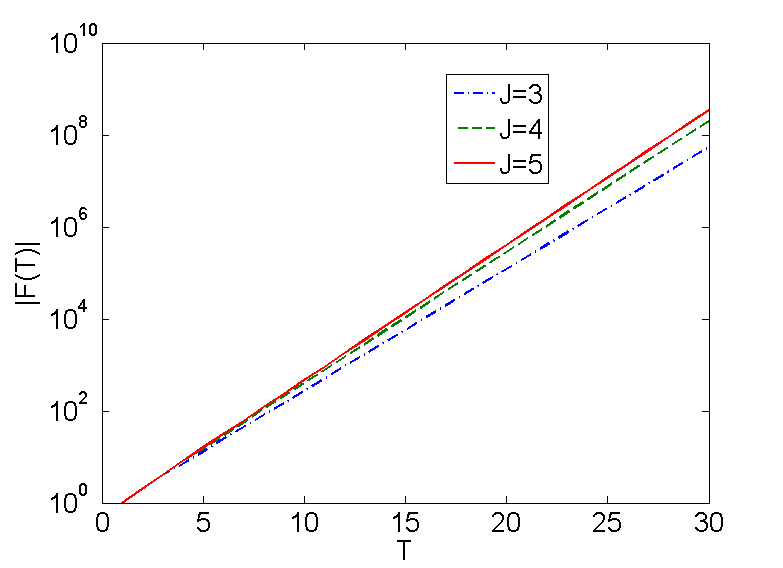
\includegraphics[scale=0.4]{iccsa2015/figures/numberfeasiblelogy.png} % escala semilogaritmica
%\includegraphics[scale=0.5]{numberfeasible.png} %escala normal (equi)
\caption{ $|F(T)|$ as a function of $T$ and several values of the shelf life $J$.}
\label{fig:numberfeasible}
\end{figure}

\begin{equation}
\label{eq:numberfeasibleY(T)}
|F_{T+1}|= 2|F_{T}| -|F_{T-J}|
\end{equation}
with the initial terms  $|F_{t}|=2^{t-1}, \  t<J+1$, and  $|F_{J+1}|=2^J-1 $
\end{proposition}

\begin{proof}
Consider $p=(p_1,\ldots,p_{T})\in F_{T}$, then obviously $(p_1,\ldots,p_{T},1)\in F_{T+1}$. We now focus on the case of $(p,0)=(p_1,\ldots,p_{T},0)$. Its feasibility is determined by the values of $p_{T-(J-2)},\ldots, p_{T-1},p_T$. Let $\boldsymbol{0}$ be now an all zeros vector with $J-1$ elements. If $(p_{T-(J-2)},\ldots, p_{T-1},p_T)=\boldsymbol{0}$, then $(p,0)$ is not feasible. But how many feasible $p\in F_{T}$ exist with this feature?

Given $(p_{T-(J-2)},\ldots, p_{T-1},p_T)=\boldsymbol{0}$ and $p\in F_{T}$, we must have $p_{T-J+1}=1$. There are $|F_{T-J}|$ feasible timing vectors $(p_1,\ldots,p_{T-J})$ with $(p_1,\ldots,p_{T-J},1,\boldsymbol{0})$  feasible and  $(p_1,\ldots,p_{T-J},1,\boldsymbol{0},0)$ infeasible.
From this follows the final result, $|F_{T+1}|= 2|F_{T}| -|F_{T-J}|$.
%\qed
\end{proof}




The proof of Proposition~\ref{prop:numberfeasible} gives a constructive method to determine all feasible policies recursively. Moreover, (\ref{eq:numberfeasibleY(T)}) shows that the space of feasible policies grows exponentially with $T$ as illustrated in Figure~\ref{fig:numberfeasible}.



\subsection{Basic Order Quantities}
\label{sec:safe}
We focus now on the minimum order quantity at period $t\in \{1,\ldots,T\}$  to cover demand for the next $r$ periods $t, t+1,\ldots, t+r-1$ that is just sufficient according to the service level constraint where at period $t$ no older items are in stock.
\begin{figure}[h]
\centering
%\includegraphics[scale=0.5]{lossfunction.png}
\includegraphics[scale=0.4]{iccsa2015/figures/lossfunFig.png}
%\includegraphics[scale=0.5]{lossfunFig.pdf}
\caption{One period loss function $E(X|Q)$ for $\boldsymbol d \sim N(1950,0.25\cdot1950)$ and corresponding basic order quantity $q$: $E(X|q)=(1-\beta)\mu$}
\label{fig:lossfunFig}
\end{figure}
\begin{defn}
Basic order quantity $\overline Q_{r,t}$ is the amount for period $t$ that fulfils constraint (\ref{eq:chanceICCSA}) for the next $r$ periods: $t,t+1,\ldots,t+r-1$.
\end{defn}
We first consider $\overline Q_{1t}$. Let the replenishment cycle be one period $R=1$, zero inventory and $q$ the order quantity. In this case, lost sales $X$ from expression (\ref{eq:lostsalesICCSA}) can be simplified to:
%
\begin{equation}
\boldsymbol{X}=\left(\boldsymbol{d}-q\right)^+ .
\end{equation}
Let $\varphi$ be the density function (pdf) of $\boldsymbol d$ and $\Phi$ be the corresponding cumulative distribution function (cdf).
%
%
Then the so-called loss function expressing the expected lost sales as a function of $q$ is
%
\begin{equation}
L(q) = E(\boldsymbol{X})=E\left((\boldsymbol{d}-q)^+\right)= \int\limits_{q}^{\infty} (x-q)\varphi(x)dx,
\end{equation}
%
where the symbol $x$ is used here as the argument in the integral. The cost function (\ref{eq:objICCSA}) is monotonously increasing in the order quantity $q$ and $L(q)$ decreases, so constraint (\ref{eq:chanceICCSA}) is binding for the optimal value of $q$ such that $L(q) = (1-\beta) \mu$ as illustrated in Figure~\ref{fig:lossfunFig}. Since demand is normally distributed, there is no closed-form expression for the first order loss function.  Some approximations for the loss function can be found in  \cite{kurawarwala96},\cite{Rossi14},\cite{DeSchrijver20121375},\cite{Waissi199691}. From a root-finding perspective, there are several ways to proceed (see \cite{HENTO10}). For instance, one can use the derivative of loss function  $L'(q)=\int\limits_{-\infty}^{q}\varphi(x)dx - 1 = \Phi(q) - 1$ to approximate $q$ using \emph{Newton-Raphson} method. The following theoretical result shows that for the described model, the determination of $q$ has to be done only once.
%
\begin{lemma}
\label{lem:q1}
Let $\boldsymbol{d}\sim N(\mu,cv\times \mu)$ and $\varphi$ be the pdf and $\Phi$ the cdf of the standard normal distribution. The solution of  $L(q) = (1-\beta) \mu$ fulfils $q=\mu(1+cv\times\hat x)$ where $\hat x$ solves
$\varphi\left(\hat x\right)-\left(1-\Phi\left(\hat x\right)\right)\hat x =\frac{1-\beta}{cv}$.
\end{lemma}
%
\begin{proof}
Using the results in \cite{Rossi14} for $\boldsymbol{d}\sim N(\mu,cv\times\mu)$,  the loss function can be expressed as
%
\begin{equation}
\label{eq:rossi}
L(q)=cv\times\mu \left(\varphi\left(\frac{q-\mu}{cv\cdot\mu}\right)-\left(1-\Phi\left(\frac{q-\mu}{cv\cdot\mu}\right)\right)\frac{q-\mu}{cv\cdot\mu}\right) .
 \end{equation}
The Equation $L(q)=(1-\beta)\mu$ substituting $q=\mu(1+cv\times\hat x)$ implies
%
\begin{equation}
\label{eq:rossi2}
 \varphi\left(\frac{q-\mu}{cv\cdot \mu}\right)-\left(1-\Phi\left(\frac{q-\mu}{cv\cdot \mu}\right)\right)\frac{q-\mu}{cv\cdot \mu} =
\varphi(\hat x)-(1-\Phi(\hat x))\hat x =
 \frac{1-\beta}{cv} .
 \end{equation}
%\qed
\end{proof}
%
\begin{figure}[!bt]
\centering
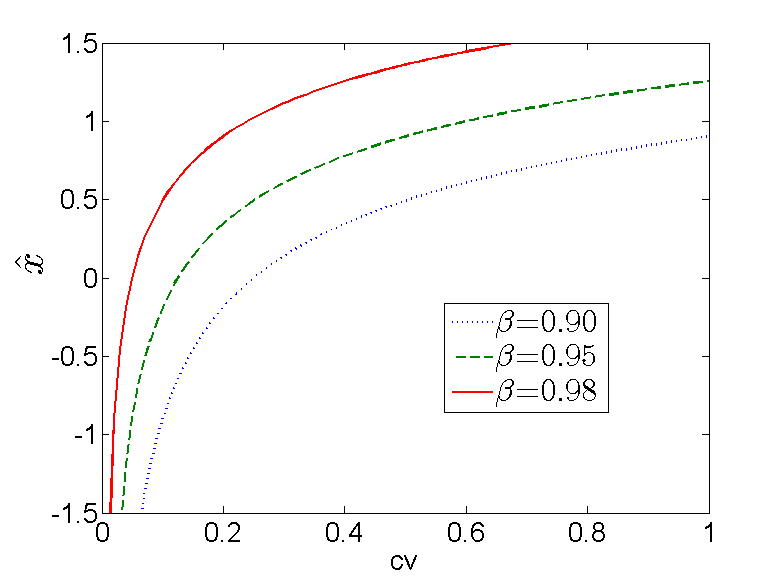
\includegraphics[scale=0.4]{iccsa2015/figures/xhat_ncvnew.png}
%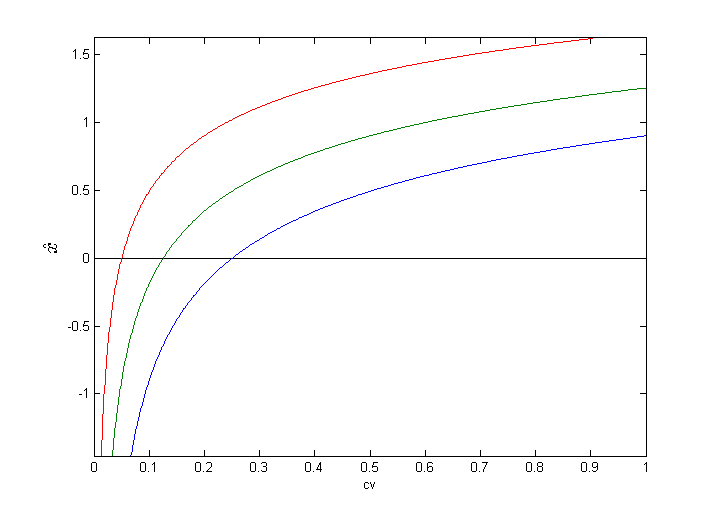
\includegraphics[scale=0.4]{xhat_ncv.pdf}
\caption{Solution $\hat x$ of (\ref{eq:rossi2}) as function of $cv$ for several values of $\beta=0.90, \ 0.95, \ 0.98$ %(blue) $\beta=0.95$ (green) and $\beta=0.98$ (red)
}
\label{fig:xhat_ncv}
\end{figure}
%
The basic order quantity $\overline Q_{1t}= \mu_t(1+cv\times\hat x)$ provides an upper bound on the order quantity $Q_t$ if $R_t=1$, because inventory may be available. Figure~\ref{fig:xhat_ncv} shows the relation of $\hat x$ with parameters $cv$ and $\beta$. Its value indicates how much bigger (smaller if negative) the basic quantity is compared to $\mu$.

The basic order quantities for longer replenishment cycles look more complicated. For instance, $R_t=2$ implies
$$E\left(\boldsymbol{d}_{t+1}-(\overline Q_{2t}-\boldsymbol{d}_{t})^+)\right)^+=(1-\beta)\mu_{t+1} .$$ 
%
These expressions become more cumbersome with the size of the replenishment period. To solve them we need a different approach.
%
Consider a replenishment cycle of $r$ periods, from $t_1$ to $t_2$ with $t_2=t_1+r-1$ and $\boldsymbol{d_{t_1,t_2}} = \boldsymbol {d_{t_1}} + \ldots + \boldsymbol {d_{t_2}}$.  Let $\varphi_{t_1,t_2}$ be the density function (pdf) of $\boldsymbol d_{t_1,t_2}$ and $\Phi_{t_1,t_2}$ be the corresponding cumulative distribution function (cdf). As we are considering that demand is normally distributed, the distribution of $\boldsymbol d_{t_1,t_2}$ is normal as well, with expected value $\mu=\mu_{t_1} + \ldots + \mu_{t_2}$ and $\sigma=cv \sqrt{\mu^2_{t_1} + \ldots+\mu^2_{t_2}}$. Starting with $q$ units at period $t_1$, the expected value of the sum of lost sales from periods $t_1$ to $t_2$, $SL_{t_1,t_2}(q)$ is determined by
\begin{equation}
\label{eq:sumloss}
SL_{t_1,t_2}(q)=E\left(\sum\limits_{i=t_1}^{i=t_2}X_i\right) =E\left((\boldsymbol{d_{t_1,t_2}}-q)^+\right)= \int\limits_{q}^{\infty} (x-q)\varphi_{t_1,t_2}(x)dx.
\end{equation}
Following the considerations in \cite{Rossi14}, $SL_{t_1,t_2}(q)$ can be expressed as
%
\begin{equation}
\label{eq:rossitotloss}
SL_{t_1,t_2}(q)=\mu-q+\sigma\varphi\left(\frac{q-\mu}{\sigma}\right)+\Phi\left(\frac{q-\mu}{\sigma}\right)(q-\mu).
 \end{equation}
% where $\mu=\mu_{t_1} + \ldots + \mu_{t_2}$ and $\sigma=cv \sqrt{\mu^2_{t_1} + \ldots+\mu^2_{t_2}}$.
Now consider the expected lost sales $L_{t_1,t_2}(q)$ in period $t_2$ when $q$ fresh units are available at the beginning of period $t_1$. The quantity follows from subtracting from the expected total lost sales up to period $t_2$ in (\ref{eq:sumloss}) the expected value of total lost sales from periods $t_1$ to $t_2 -1$
\begin{eqnarray}
\label{eq:lostsalesgeneral}
L_{t_1,t_2}(q)&=& SL_{t_1,t_2}(q)- SL_{t_1,t_2-1}(q) = \\ \nonumber
&&=\int\limits_{q}^{\infty} (x-q)\left(\varphi_{t_1,t_2}(x)-\varphi_{t_1,t_2-1}(x)\right)dx.
\end{eqnarray}
To find the value $q_{rt}$ for which the service level constraint is just fulfilled in period $t_2=t+r-1$ when having $q_{rt}$ fresh units at the beginning of period $t$ follows from solving $L(q_{1t})=(1-\beta)\mu_t$ according to Lemma \ref{lem:q1} and for $r>1$ one can solve
\begin{equation}
\label{eq:partialbasic}
SL_{t,t+r-1}(q_{rt})-SL_{t,t+r-2}(q_{rt})=(1-\beta)\mu_{t+r-1}
 \end{equation}
 for $q_{rt}$. The basic order quantity $\overline Q_{rt}$ now follows from taking the maximum of these quantities $\overline Q_{rt}=\max_{j=1,\ldots,r}q_{jt}$, such that the service level constraint is fulfilled in all periods of the replenishment cycle. The values of the basic order quantities in Table %\ref{tab:demand}
 \ref{tab:Ybasicorder} follow from the parameter values in Example \ref{ex:mainexample}.
%%%%%%



\begin{example}
\label{ex:mainexample}

Consider an instance of the problem with $T=12$ periods and shelf life $J=3$. Random variables of demand for every period are expressed in terms of their mean values $\mu_t$ given in last row of Table \ref{tab:Ybasicorder} and the coefficient of variation is given by $cv=0.25$. The required service level is $\beta=95\%$, such that the value of $\hat x$ in Lemma \ref{lem:q1} is $\hat x=0.493$. This value can be used, by Lemma \ref{lem:q1}, to determine the values for $\overline Q_{1t}$ in the first row of Table  \ref{tab:Ybasicorder}. Solving (\ref{eq:partialbasic}) and taking  $\overline Q_{rt}=\max_{j=1,\ldots,r}q_{jt}$ provides values for $\overline Q_{rt}$ for $r>1$ in Table \ref{tab:Ybasicorder}. The values are rounded up.
%
\end{example}



\begin{table}[h]
	\caption{Basic order quantities}
	\label{tab:Ybasicorder}
	\centering
	\resizebox{0.9\columnwidth}{!}{
		\begin{tabular}{@{}lrrrrrrrrrrrr@{}}
			\toprule
			r$\setminus$t        & \multicolumn{1}{c}{1} & \multicolumn{1}{c}{2} & \multicolumn{1}{c}{3} & \multicolumn{1}{c}{4} & \multicolumn{1}{c}{5} & \multicolumn{1}{c}{6} & \multicolumn{1}{c}{7} & \multicolumn{1}{c}{8} & \multicolumn{1}{c}{9} & \multicolumn{1}{c}{10} & \multicolumn{1}{c}{11} & \multicolumn{1}{c}{12} \\ \midrule
			1 & \textbf{898}          & 1067                  & 224                   & 1010                  & 898                   & \textbf{168}          & 730                   & 898                   & \textbf{1010}         & \textbf{336}           & 168                    & 673                    \\
			2 & 1952                  & \textbf{1450}         & 1211                  & \textbf{1925}         & 1225                  & 885                   & \textbf{1618}         & 1898                  & 1458                  & 529                    & \textbf{825}           & 0                      \\
			3 & 2372                  & 2277                  & 2131                  & 2287                  & 1812                  & 1769                  & 2596                  & 2386                  & 1666                  & 1145                   & 0                      & 0                      \\ \midrule
			$\mu_t$  & 800                   & 950                   & 200                   & 900                   & 800                   & 150                   & 650                   & 800                   & 900                   & 300                    & 150                    & 600
		\end{tabular}
	}
\end{table}

\subsection{Optimal Quantities for a Given $Y$}
\label{sec:nlp}
So far, we have described a method to find a feasible $Q$ vector for a given $Y$, using the so called Basic order quantities. Now we can define a method to optimize the objective function (\ref{eq:objICCSA}) subject to a given timing vector $Y$.

We consider now the properties of the MINLP problem described in Section \ref{sec:model}. We first focus on the monotonicity of the objective function in the order quantities when $w>-c$ applies.



\begin{lemma}
\label{lem:finalg}
Given an order timing vector $Y$ with corresponding values $A$ and $M$ according to Definition \ref{def:A}, if $Q^*(Y)$ is an optimal solution of (\ref{eq:objICCSA}),(\ref{eq:procICCSA}),(\ref{eq:invWasteICCSA}), (\ref{eq:inv2ICCSA}), (\ref{eq:inv1ICCSA}), (\ref{eq:lostsalesICCSA}) and (\ref{eq:defg}) with $Q_t= 0$ if $Y_t=0$ then $g_{T}(Q^*)=0$ .%\nonumber.
\end{lemma}
\begin{proof}
Assume $Q^ *$ is optimal and $g_{T}(Q^*)<0$. Due to the inventory dynamics and $g_T$ being a continuous function in its arguments, $\exists \epsilon>0$ such that $Q=Q^*-\epsilon e_{A_M}$ is a feasible solution with $g_{T}(Q)=0$. Due to the FIFO dynamics $I_{jt}(Q)\le I_{jt}(Q^*), j=1,\ldots,J$ and specifically $I_{Jt}(Q^*)-I_{Jt}(Q)\le \epsilon$. As also $\sum Q_t-\sum Q_t^* =\epsilon$ we have that $f(Q)\le f(Q^*)-(c-w)\epsilon < f(Q^*)$ which contradicts $Q^*$ can be optimal with $g_{T}(Q^*)<0$.  
\end{proof}



\begin{proposition}
\label{prop:optimizeY}
Given an order timing vector $Y$ with corresponding values $A$ according to Definition \ref{def:A} and $M=\sum Y_t$.   If $Q^*(Y)$ is an optimal solution of (\ref{eq:objICCSA}),(\ref{eq:procICCSA}),(\ref{eq:invWasteICCSA}), (\ref{eq:inv2ICCSA}), (\ref{eq:inv1ICCSA}), (\ref{eq:lostsalesICCSA}) and (\ref{eq:defg}) with $Q_t= 0$ if $Y_t=0$ then (\ref{eq:defg}) is binding for $t=A_i -1, i=2,\ldots,M$ and $t=T$:
\begin{equation}
\label{eq:optimalQ}
%Q^* =(Q_1^*,\ldots, Q_{T}^*)= min_Q f(Q_1 ,\ldots, Q_{T})\\
 %\text{ s.t. }
 g_{A_2-1}(Q^*) = \ldots = g_{A_M-1}(Q^*)= g_{T}(Q^*)=0 .%\nonumber.
\end{equation}
\end{proposition}
\begin{proof}
Follows from applying the proof of Lemma \ref{lem:finalg} in a sequential way. Lemma \ref{lem:finalg} has shown that $g_{T}(Q^*)=0$. Assume $Q^*$ is optimal with $g_{A_M-1}(Q^*)<0$. As $g_{A_M-1}$ is a continuous function in $Q$, $\exists \epsilon>0$ such that for $Q=Q^*-\epsilon e_{A_{M-1}}$ 
we still have $g_{A_M-1}(Q)<0$. If $R_{M-1}=J$, we have that less items perish at the end of the cycle for $Q$ than for $Q^*$ and therefore $f(Q)<f(Q^*)$ leading to a contradiction.

However, if $R_{M-1}<J$ less inventory $\mathcal{I}(Q)=\sum_{j=R_{M-1}}^{J-1}I_j(Q)$ is available at the end of the cycle and $Q^*_M$ has to be increased to meet the constraint for the last period. \cite{Rossi14} show that the so called complementary loss function $E(\mathcal{I}(Q))$ is strictly convex with partial derivatives less than 1. This implies that $\delta= E(\mathcal{I}(Q^*))-E(\mathcal{I}(Q))<\epsilon$. Consequently there exists a feasible solution $Q^* -\epsilon e_{A_{M-1}} +\delta e_{A_{M}}$ that has lower cost than $Q^*$. This contradicts the assumption. By following this reasoning backward, it is shown that for all periods at the end of a replenishment cycle constraint (\ref{eq:defg}) has to be binding.%\qed   
\end{proof}

Finding (\ref{eq:optimalQ}) implicitly gives a way to determine $Q^*(Y)$. Minimise the quantity of the first cycle up to constraint (\ref{eq:chanceICCSA}) is fulfilled and proceeding with the next cycle until the last one. Notice that given $Y$, the optimal quantities do not depend on the parameter values of the objective function (\ref{eq:objICCSA}).



\section{Algorithms for Generating Order Quantities}
\label{sec:alg}

The derived basic order quantities can now be used to obtain feasible solutions and to improve them towards optimal solutions.

\subsection{Generating a Feasible Solution for a Given $Y$}
Given a list of order periods $Y$ one can determine a feasible solution $Q$ based on $\overline{Q}_{r,t}$.  After determination of $A$ and $R$ from Definitions \ref{def:A} and \ref{def:R}, the appropriate values can be assigned. Example \ref{ex:feasiblesolY} shows a case for a vector $Y$.


\begin{example}
\label{ex:feasiblesolY}
Consider the data and variables of Example \ref{ex:mainexample}. One can determine a feasible solution $Q_t$ for a given timing vector $Y$ using the basic order quantities $\overline Q_{r,t}$. For timing vector $Y=(1,1,0,1,0,1,1,0,1,1,1,0)$, vectors $A$ and $R$ are defined by: $A=(1,2,4,6,7,9,10,11)$ and $R=(1,2,2,1,2,1,1,2)$. Selecting the appropriate basic order quantities results into  $Q=(898,1450,0,$ $1925,0,168,$ $1618,0,1010,$ $336,825,0)$ as illustrated in Table \ref{tab:Ybasicorder}.
\end{example}




\subsection{Generating the Optimal Solution for a Given $Y$}
\begin{algorithm}[h]
	\caption{MinQ($Y$): Optimal order quantity $Q$ for $Y$}
	\label{alg:optimalforYICCSA}
	\begin{algorithmic}[1]
		%\Procedure{MinQ}{$Y$}
        \REQUIRE Orders timing $Y$, fixed shelf life $J$ 
        \ENSURE Optimal order quantity $Q$ for $Y$
        \medskip
		\STATE Determine replenishment periods $A(Y)$, Definition \ref{def:A} 
        \STATE Determine corresponding replenishment cycles $R$, Definition \ref{def:R} 
		\FOR {$i=1$ \textbf{to} $\sum_t Y_t$ } % For every vector of order periods for $Y$
        \IF  { ($A_i=1$ \textbf{or} $A_i -  A_{i-1}=J$) }  %[Inventory is zero] %\hfill \#Inventory is zero
		\STATE $Q_i=Q_{R_i,A_i}$; \label{optimalforY:line:beforeflossICCSA} \hfill \#minimum value for constraint~(\ref{eq:chanceICCSA})
		\STATE  $(z,I_{A_i+R_i-1})=$\textbf{floss}($Q_i,A_i,A_i+R_i-1,0$) \label{optimalforY:line:flossICCSA} \hfill \# Alg. \ref{alg:simulation} updates inventory $I$
		\ELSE
        \STATE $Q_i=$ \textbf{Ordervalue}($A_i,R_i,I_{A_i-1}$) \hfill \# Algorithm~\ref{alg:ordervalueICCSA}
		\ENDIF
		\ENDFOR
		%\EndProcedure
		\vskip 5pt
	\end{algorithmic}
	
\end{algorithm}
The process of optimizing quantities for a timing vector $Y$ is sketched at Algorithm \ref{alg:optimalforYICCSA}. Proposition \ref{prop:optimizeY} shows with (\ref{eq:optimalQ}) that the quantities for the order periods of $Y$ can be calculated sequentially from $A_1=1$  to $A_M$, $M=\sum\limits_{t=1}^{T}Y_t$. 
\begin{algorithm}[h]
	\caption{floss($q$,$t_1,t_2,I$): Monte Carlo sim, estimates  $E(\boldsymbol{X})$, updates $\boldsymbol{I_{t_2}}$}
	\label{alg:simulationICCSA}
	\begin{algorithmic}[1]
        \REQUIRE Order quantity ($q$), time window $[t_1,t_2]$, number of sample paths $N$%, fixed shelf life ($J$)
        , sample starting inventory $I_{jn}, j=1,\ldots,J-1, n=1,\ldots,N$%, $\mu_t, t\in[t_1,t_2]$, $cv$
        \ENSURE  Estimate $Z$ of $E(X_{t_2})$, a sample of $I_{t_2}$
        \medskip
		\FOR{$n=1$ \textbf{to} $N$}
		\STATE $I_{1,t,n}= \left(q - (d_{t_1,n}-\sum_{j=1}^{J-1}I_{jn})^+\right)^+$; %\hfill \#Update inventory ($I$)
			\FOR{$t=t_1$ \textbf{to} $t_2$}
				\FOR{$j=2$ \textbf{to} $j=J-1$ }
					\STATE $I_{j,t,n}= \left(I_{j-1,t-1,n} - (d_{t,n}-\sum_{k=j}^{J-1}I_{k,t-1,n})^+\right)^+$; \hfill \#Update inventory ($I$)
				\ENDFOR
				\ENDFOR
				
				%\STATE $I_{J,t,n}=(I_{J-1,t-1,n} - d_{t,n})^+$
				\STATE $Z=\frac{1}{N}\sum\limits_{n=1}^{N} \left(d_{t_2,n}-\sum_{j=1}^{J-1}I_{j,t_2-1,n}-q\right)^+$; \hfill %\#Update lost sales $X$	
		\ENDFOR
		\vskip 5pt
	\end{algorithmic}
	
\end{algorithm}
\noindent If a replenishment period $A_i$ is preceded by $J-1$ periods without replenishment, the inventory perishes and starting inventory at $A_i$ is equal to zero. For those cases basic order quantity $Q_{R_i,A_i}$ with $R_i$ the length of the replenishment cycle $i$, is optimal. When period $A_i$ is preceded by less than $J-1$ no-replenishment periods, the optimal order quantity is lower than the basic order quantity, due to random inventory $\boldsymbol{I}_{1,A_{i}-1}\ldots,\boldsymbol{I}_{J-1,A_{i}-1}$. The minimum order quantity that just fulfils (\ref{eq:chanceICCSA}) can be determined by simulation.


Algorithm~\ref{alg:simulationICCSA} estimates expected lost sales and determines the end inventory based on Monte Carlo simulation. Function \textbf{floss}($q$,$t_1$,$t_2,I$)  consists of simulating inventory for $N$ demand paths and determines lost sales of period  $t_2$ given order quantity $q$ at period $t_1$. In Algorithm \ref{alg:optimalforYICCSA} (line~\ref{optimalforY:line:flossICCSA}), when starting inventory is zero and the order quantity is a basic order quantity (line~\ref{optimalforY:line:beforeflossICCSA}), Algorithm~\ref{alg:simulationICCSA} is also run to determine the inventory $I$ at the end of the cycle, i.e. period $t_2$. The value of $N$ must be large enough to provide accurate estimates for the expected lost sales.


To determine the order quantity such that (\ref{eq:defg}) is binding when the starting inventory is nonzero, an approach can be used as sketched in Algorithm \ref{alg:ordervalueICCSA} based on the secant method (lines 5-8). It takes replenishment cycle $[t_1,t_2=t_1+r-1]$ as input, where $r$ is the length of the cycle and a starting inventory $I$.
Iteratively, function $\textbf{floss}(q,t_1,t_2,I)$ is evaluated to determine expected loss at the end of the cycle. %Example \ref{ex:ex3} shows how Algorithm \ref{alg:ordervalue} helps to reduce the order quantities for a timing vector.


 \begin{algorithm}[h]
 \caption{Ordervalue($t_1$,$t_2,I$): Determines an order quantity fulfilling (\ref{eq:chanceICCSA})}
 \label{alg:ordervalueICCSA}
 \begin{algorithmic}[1]
 %\Procedure{ordervalue}{$t_1,t_2$}
 %\State $t_2=t_1 + r - 1$
 \REQUIRE Time window $[t_1,t_2]$, sample starting inventory $I_{jn}, j=1,\ldots,J-1, n=1,\ldots,N$, required fill rate $\beta$, accuracy $\epsilon$
 \ENSURE Order quantity $q$
 \medskip
 \STATE $K=(1-\beta) \mu_{t_2}$; \hfill \#Target level
 \STATE Choose two initial order quantities $q_1$ and $q_2$; \hfill \#Secant method
 \STATE $(z_1,I_{t_2}) = \textbf{floss}(q_1,t_1,t_2,I)$ and  $(z_2,I_{t_2}) = \textbf{floss}(q_2,t_1,t_2,I)$; \hfill \# Algorithm~\ref{alg:simulationICCSA}
 \WHILE  {$|z_2 - K| >\epsilon$}
 \STATE $q = q_1 + \frac{(K-z_1)(q_2-q_1)}{z_2-z_1}$;
 \STATE $z_1 = z_2$;
 \STATE $z_2 = \textbf{floss}(q,t_1,t_2,I)$; \hfill  \# Algorithm~\ref{alg:simulationICCSA}
 \STATE $q_1 = q_2$; $q_2 = q$;
 \ENDWHILE
%\STATE\RETURN $q$
 %\EndProcedure
 \vskip 5pt
 \end{algorithmic}
 \end{algorithm}


\begin{example}
\label{ex:ex3}
	Consider timing vector $Y$ of Example \ref{ex:feasiblesolY} and corresponding feasible order quantities  $Q=(898,1450,0,$ $1925,0,168,$ $1618,0,1010,$ $336,825,0)$, Algorithm \ref{alg:ordervalueICCSA} reduces these values to $Q= (898,1379,$ $0,1670,0,120,$ $1536,0,879,$ $273,726,0)$.
\end{example}

\subsection{Algorithm for the Global Optimum Solution}

Given Algorithm \ref{alg:optimalforYICCSA} to optimize quantities $Q$ given timing vector $Y$, the question is how to find the optimal timing $Y^*$ of the MINLP problem of Section \ref{sec:model}. This is done by a systematic enumeration of feasible  orders timing vectors $Y$  and evaluating the objective function (\ref{eq:objICCSA}). By Lemma \ref{lem:Y}, infeasible  orders timing vectors can be discarded. Furthermore, a lower bound on the cost function can be used to leave out more orders timing vectors for which the lower bound is higher than the cost of the best solution found thus far.

\subsubsection{Determination of a lower bound on the cost function for each $Y$}
\label{sec:lowerbound}
Let $Y$ be a feasible timing vector. The ordering cost for $Y$ is known to be $k \sum\limits_{t=1}^{T}Y_t$. Suppose $t$ is an order period for a cycle $R>1$.  To fulfil the $\beta$ service level, the minimum remaining stock to be stored at periods $t$, $t+1$,\ldots, $t+R-1$ is given by  $\overline Q_{R,t+1}$,\ldots,$\overline Q_{1,t+R}$ respectively. Notice that the basic order quantity is the minimum amount needed to fulfil demand for a sequence of periods. Based on these considerations, a lower bound on the cost function for $Y$ can be calculated.

\begin{algorithm}[h]
\caption{AllY(): Evaluating all feasible timing vectors $Y$}
\label{alg:bestYICCSA}
\begin{algorithmic}[1]
%\Procedure{AllY}{ }
 \REQUIRE All feasible $Y$'s
 \ENSURE The optimal timing vector ($Y^*$) and order quantities ($Q^*$)
 \medskip
\STATE mincost=$\infty$
\FOR{all $Y$}
\IF{lower bound ($Y$) $<$ mincost}  \label{bestY:line:LB}
\STATE $Q_Y$=  \textbf{MinQ}(Y);   \label{bestY:line:NLPsolver} \hfill \# Algorithm \ref{alg:optimalforYICCSA}
\STATE $C(Q_Y)$; \hfill \#Determine the cost of $Q_Y$
\IF{$C(Q_Y)<$mincost}
\STATE mincost=$C(Q_Y)$;
\STATE $Y^*=Y$;
\ENDIF
\ENDIF
\ENDFOR
%\EndProcedure
\vskip 5pt
\end{algorithmic}
\end{algorithm}

\subsubsection{Determination of the optimal timing vector $Y^*$ and order quantities $Q(Y^*)$}
Algorithm \ref{alg:bestYICCSA} determines the optimal timing vector $Y$ and the optimal production quantities by enumerating and testing feasible timing. Using the lower bound described some or many of the feasible policies can be discarded, depending on the cost parameters. For each feasible $Y$, such that  $lower$ $bound(Y) < mincost$, Algorithm~\ref{alg:optimalforYICCSA}  provides the  optimal production quantities $Q^*=Q(Y^*)$. Alternatively step \ref{bestY:line:NLPsolver} can also be done by a standard NLP algorithm.


{\color{black}{The computational burden of Algorithm \ref{alg:bestYICCSA} is related to the number of feasible policies $Y$, which is exponential in $T$, i.e. $O(2^T)$. Moreover, the hardness for each timing $Y$ is related to the number simulated periods by Algorithm \ref{alg:ordervalueICCSA}, which is also bounded by $T$. Evaluation of {\bf floss} requires simulating $N$ demand paths (Algorithm \ref{alg:simulationICCSA}). Summarizing, the total computational burden for finding the  best timing vector $Y^*$ and corresponding orders $Q(Y^*)$ is in the order $O(N \cdot T \cdot 2^T)$.}


\section{Parameter Sensitivity of the Optimal Solution}
\label{sec:parameters}
This section analyses the effect of the value of the parameters of the objective function on the optimal orders quantities. This analysis will help to better understand the cost associated to the service level quality  (value of $\beta$) as well as the uncertainty of demand (measured by $cv$).

\subsection{Effects of Parameters $\beta$ and $cv$}
First, we focus on the parameters that determine the basic order quantities to fulfil the $\beta$-service level  constraint. For a replenishment cycle of length $R$, the basic order quantity depends on parameters $\beta$ and $cv$. Section \ref{sec:safe} shows that the loss function for the last period of the cycle approaches zero, i.e. $\lim \limits_{q \to \infty}L(q)=0$. The basic order quantity $q$, for which $L(q)=(1-\beta)\mu$, typically goes up with the requirement $\beta \in [0,1)$ and ${q}\rightarrow \infty$ when $\beta \rightarrow 1$ as illustrated in Figure \ref{fig:qnbeta}.


\begin{figure}[!ht]
\centering
\includegraphics[scale=0.50]{iccsa2015/figures/qnbeta.png}
%\includegraphics[scale=0.3]{qnbeta.pdf}
\caption{Basic order quantity $q$ as function of $\beta$ for $cv \rightarrow 0$ (blue), $cv=0.25$ (green) and $cv=0.33$ (red)}
\label{fig:qnbeta}
\end{figure}

Similarly basic order ${q}$ tends to be $(1-\beta)\mu$  when $cv \rightarrow 0$, as the normal distribution approximates a degenerate distribution at $\mu$. Figure~\ref{fig:qnbeta} also shows this effect for demand centred at $\mu=1$ and different values of $cv$: the blue line illustrates the degenerate case and the green and red curves represent $q$ as a function of $\beta$, for $cv=0.25$ and $cv=0.33$ respectively. As $cv$ grows, the distribution spreads and the order quantity has to be larger to meet the fill rate.


Obviously, when dealing with more than one period and inventory variables from previous periods the analytical expression of the loss function is different, but results show that the trend is the same.

\subsection{Cost Parameter Sensitivity}

A surprising result from Proposition \ref{prop:optimizeY} is that given a timing vector $Y$ and the assumptions on the cost parameters (positive and $c>-w$),  the optimal quantities $Q^*(Y)$ do not depend on the values of the cost parameters of (\ref{eq:objICCSA}). However, like in most inventory models (see \cite{Silver98}) there is a trade off between the order cost $k$ and the holding cost which causes the optimal timing vector $Y^*$ to depend  on specific cost parameter values.


When order cost $k=0$ or relatively low compared to other cost parameters, the optimal timing vector tends to correspond to ordering at every period. Something similar happens when $k$ is relatively high compared with the rest of parameters. In this case the optimal timing vector is to spread the orders as much as possible, every $J$ periods. This is also valid, if the distribution of demand for one or some periods has a much higher mean value than the rest. The challenging situation occurs when $k$ has a value in between the two extremes.



\section{Experiments}
\label{sec:exp}

We now evaluate the effectiveness and efficiency of Algorithm \ref{alg:bestYICCSA} using two different implementations of step \ref{bestY:line:NLPsolver} to obtain the optimal order quantity $Q$ for a given $Y$. The first one is the derived Algorithm \ref{alg:optimalforYICCSA} $MinQ(Y)$ using the presented properties of the problem. The second is the general purpose nonlinear optimization solver \emph{fmincon} of Matlab.

Example \ref{ex:mainexample} has been used as base case (see Subsection \ref{sec:safe}) considering varying values of the parameters: fill rate ($\beta=0.90, 0.95,0.98$), the coefficient of variation ($cv=0.10, 0.25, 0.33$) and the ordering cost ($k=500, 2000$). The values of the other cost parameters have been set to $c=2$, $h=0.5$ and $w=0$ for all the runs. For the evaluation of the costs,  $N=5000$ demand paths (Monte Carlo simulations) are used. Notice that the same pseudo random numbers for the demand have been used, allowing comparison of the obtained order policy for both solvers. For the same reason,  \emph{fmincon} and Algorithm  \ref{alg:ordervalueICCSA}  use the same termination tolerance ($\epsilon=10^{-6}$)  for constraint~(\ref{eq:defg}).

Using these settings, for each feasible timing vector $Y$, the order quantities computed by both methods match up to at least the first five digits. According to Proposition \ref{prop:optimizeY}, the procedure Algorithm  \ref{alg:ordervalueICCSA} also should lead to the optimal solution. The fact that a practical general purpose solver reaches the same optimum shows that the underlying problem does not exhibit numerical instabilities. 

For every possible combination of the considered values of $\beta$, $cv$ and $k$, the optimal value of the objective function (\ref{eq:objICCSA}) and the number of orders of the optimal $Y^*$ have been calculated. Figure~\ref{fig:tests} shows the optimal cost  versus the number of orders ($\sum Y^*$) for each considered problem. This figure illustrates the following aspects:
\begin{enumerate}
	\item Naturally, a lower value of $k$ provides lower optimal total costs.
	\item The value of the optimal cost increases with the requirement $\beta$ as well as with the coefficient of variation $cv$. This is a consequence of the effect of $\beta$ and $cv$ on the basic order quantities, as shown in  Figure~\ref{fig:qnbeta}.
	\item The number of ordering periods  for $Y^*$ increases as $k$ decreases.
	\item An increase of $\beta$ results in a reduction of the number of ordering periods  for $Y^*$. This is more evident for the cases where $k=500$, because there is a greater chance to reduce the aforementioned number of ordering periods to its limit of 4 orders for the case $T=12$ and $J=3$.
\end{enumerate}


\begin{figure}[!ht]
\centering
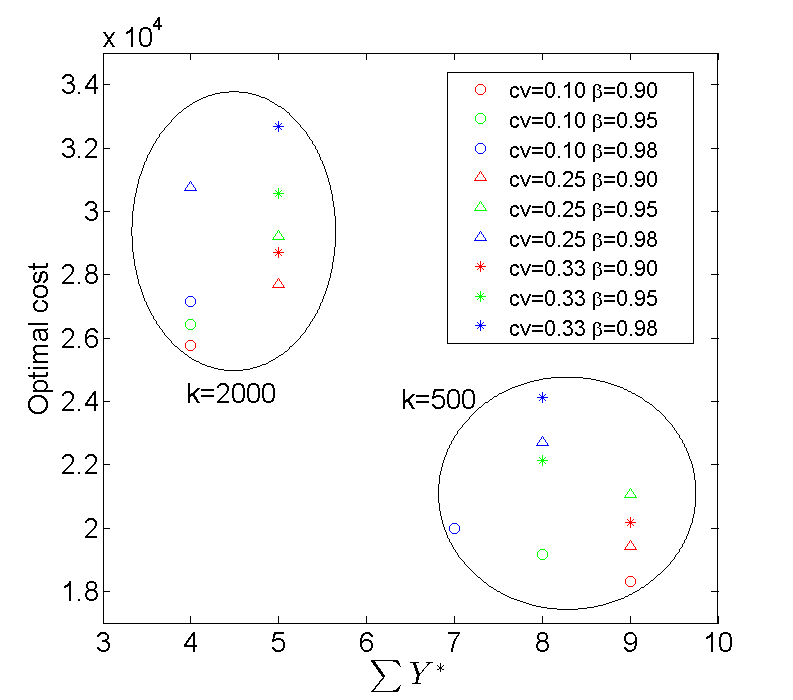
\includegraphics[scale=0.5]{iccsa2015/figures/experimentos.png}
%\includegraphics[scale=0.3]{qnbeta.pdf}
\caption{Optimal cost and number of ordering periods for every instance. Circles correspond to  $cv=0.10$, triangles to $cv=0.25$ and asterisks to $cv=0.33$. The values of $\beta=0.90$, $0.95$ and $0.98$ is represented by colors red, green and blue, respectively. $k$ identifies the ordering cost. Outcomes have been grouped according to the value of $k$.}
\label{fig:tests}
\end{figure}




With respect to efficiency, using Algorithm \ref{alg:optimalforYICCSA} (MinQ(Y)) instead of standard nonlinear optimization solver \emph{fmincon} reduces the computational time by a factor of 20. We specifically measured this for  Algorithm \ref{alg:bestYICCSA} without considering the existence of a lower bound function (line \ref{bestY:line:LB}), optimizing all feasible policies.  The main reason of the reduction is that MinQ(Y) uses all derived specific properties of the MINLP problem. 



\section{Conclusions}
\label{sec:conclusionsICCSA}
A MINLP model has been presented to determine order quantities for a perishable product inventory control problem. Basic order quantities can be determined to provide feasible production quantities for different delivery policies of the model. Theoretical properties of feasible order timings and of the NLP problem when the timing $Y$ is fixed have been derived. Based on that, a method has been developed to finding optimal quantities for the objective function (\ref{eq:objICCSA}) when the timing is given. For real applications, when $T$ is not very large, this method is able to find the optimal solution for the problem by exhaustive search of feasible policies, using a lower bound function on cost to reduce enumeration.
Moreover, obtained results have shown that the dedicated  method can reduce the runtime in a factor of $20$ with respect to the general purpose Matlab function \emph{fmincon} for solving NLP problems, while keeping the high quality of the optimal solutions.


As the NLP optimization given a timing vector $Y$ can be solved independently for each timing vector, a challenge for future investigation is to address the parallelization of the method. Such parallelization facilitates obtaining more accurate results due to a possible  increase of the number of Monte Carlo simulations to solve a particular problem and simultaneously reduces the runtime.




%--------------------------------------------------------------------------
%\section*{Appendix A: Description of the problems}
%\label{Sec:Ap}




%--------------------------------------------------------------------------
%
%\subsubsection*{Acknowledgments.}
%This paper has been supported by The Spanish Ministry  (TIN2012-37483) and Junta de Andaluc\'{\i}a (P11-TIC-7176), in part financed by the European Regional Development Fund (ERDF). The study is co-funded by the TIFN (project RE002).
%
%
%\begin{thebibliography}{1}
%\providecommand{\url}[1]{\texttt{#1}}
%\providecommand{\urlprefix}{URL }
%
%\bibitem{hedjar2004}
%Hedjar, R., Bounkhel, M., Tadj, L.: Predictive control of periodic-review
%  production inventory systems with deteriorating items. TOP  12(1),  193--208
%  (2004)
%
%\bibitem{HENTO10}
%Hendrix, E.M.T., Toth, B.G.: Introduction to Nonlinear and Global Optimization.
%  Springer, New York (2010)
%
%\bibitem{kurawarwala96}
%Kurawarwala, A.A., Matsuo, H.: Forecasting and inventory management of short
%  life-cycle products. Operations Research  44,  131--150 (1996)
%
%\bibitem{PAULS14}
%Pauls-Worm, K.G.J., Hendrix, E.M.T., Haijema, R., van~der Vorst, J.G.A.J.: An
%  {MILP} approximation for ordering perishable products with non-stationary
%  demand and service level constraints. International Journal of Production
%  Economics  157,  133--146 (2014)
%
%\bibitem{Rossi14}
%Rossi, R., Tarim, S.A., Prestwich, S., Hnich, B.: Piecewise linear lower and
%  upper bounds for the standard normal first order loss function. Applied
%  Mathematics and Computation  231,  489--502 (2014)
%
%\bibitem{Schrijver12}
%Schrijver, S.K.D., Aghezzaf, E.H., Vanmaele, H.: Double precision rational
%  approximation algorithm for the inverse standard normal first order loss
%  function. Applied Mathematics and Computation  219(3),  1375 -- 1382 (2012)
%
%\bibitem{Silver98}
%Silver, E.A., Pyke, D.F., Peterson, R.: Inventory Management and Production
%  Planning and Scheduling. Wiley (1998)
%
%\bibitem{Waissi96}
%Waissi, G.R., Rossin, D.F.: A sigmoid approximation of the standard normal
%  integral. Applied Mathematics and Computation  77(1),  91 -- 95 (1996)
%
%\end{thebibliography}
%
%
%\end{document}



%--------------------------------------------------------------------------
%\section*{Appendix A: Description of the problems}
%\label{Sec:Ap}
		
\clearemptydoublepage	
%\documentclass[review]{elsarticle}
%
%\usepackage{lineno,hyperref}
%\usepackage{epstopdf}
%\usepackage{algorithm}
%\usepackage{algpseudocode}
%\usepackage{graphicx}
%\usepackage{multirow}
%\usepackage{amsmath}
%\usepackage{booktabs}
%\usepackage{color}
%\newcommand{ 	}{\textcolor{blue}}
%\PassOptionsToPackage{hyphens}{url}
%%\usepackage{breakurl}
%
%\modulolinenumbers[5]
%
%\journal{Journal of Parallel and Distributed Computing}
%
%
%
%%% `Elsevier LaTeX' style
%\bibliographystyle{elsarticle-num}
%%%%%%%%%%%%%%%%%%%%%%%%
%
%\newcommand{\black}{\textcolor{black}}
%%\newcommand{\blue}{\textcolor{blue}}
%
%
%%\hyphenation{Ho-we-ver}
%
%\begin{document}
%
%\begin{frontmatter}
%
%\title{Accelerating an algorithm for perishable inventory control on heterogeneous platforms}
%
%  \author[add1]{Alejandro Guti\'errez-Alcoba\corref{cor1}}
%  \ead{agutierreza@uma.es}
%  \author[add2]{Gloria Ortega}
%  \ead{gloriaortega@ual.es}
%  \author[add1]{Eligius M.T. Hendrix}
%  \ead{eligius@uma.es}
%  \author[add1]{Inmaculada Garc\'ia}
%  \ead{igarciaf@uma.es}
%
%  \cortext[cor1]{Corresponding author}
%  \address[add1]{Department of Computer Architecture, \black{Escuela de Ingener\'ias, c/ Dr Ramos,  University of} M{\'a}laga, M{\'alaga}, 29071, Spain}
%  \address[add2]{Informatics Department, University of Almer\'ia, Agrifood Campus of Int. Excell. (ceiA3), Almer{\'i}a, 04120, Spain}
%
%\begin{abstract}
%This paper analyses and evaluates parallel implementations of an optimization algorithm for perishable
%inventory control problems. This iterative algorithm has high computational requirements when solving large problems. Therefore, the use of \blue{parallel and distributed computing}  reduces the execution time and improves the quality of the solutions.
%This work investigates two implementations on heterogeneous platforms: (1) a MPI-PTHREADS version; and (2) a multi-GPU version. A comparison of these implementations has been carried out. Experimental results show the
%benefits of using \blue{parallel and distributed} codes to solve this kind of problems.
%
%Furthermore, the distribution of the workload among the available processing elements is a challenging problem. This distribution of tasks can be modelled as a Bin-Packing problem. This implies that the selection of the set of tasks assigned to every processing element requires  the design of
%a heuristic capable of efficiently balancing the  workload statically with no significant overhead. This heuristic has been used for the parallel implementations of the optimization for perishable
%inventory control problem.
%\end{abstract}
%
%\begin{keyword}
%Perishable inventory control, GPU computing, Heterogeneous computing,  Optimization, Monte Carlo simulation, Bin-Packing problem
%\end{keyword}
%
%
%\end{frontmatter}
%
%\linenumbers

\chapter{Accelerating an algorithm for perishable inventory control on heterogeneous platforms} % top level followed by section, subsection
\label{Chap:jpdc}

\section{Introduction}



The main objective of this work consists of determining up to what extent the use of heterogeneous platforms (multicore and multi-GPU) accelerates the solution process
of a novel optimization algorithm
for an inventory control problem of perishable products. Our goal is to study how to take advantage of the computing capacity of these architectures to obtain more accurate solutions when large problems are considered, which imply high computational demand, keeping a reasonable response time.






The perishable inventory control problem %\blue{
presented in this chapter %}
 is defined over a finite horizon of $T$ periods of a perishable product in which a fixed percentage of the non-stationary stochastic demand has to be satisfied according to a so-called fill rate service level requirement. The perishable product has a fixed shelf life of $J$ periods. In the modeling of this problem, it is supposed that $J<T$ and the dynamics of the inventory follows the FIFO issuance (first in, first out), in which the oldest product is issued first.
Items of age $J$ cannot be used in the next period and are considered waste. The goal is to %find what service level is optimal, in the sense of
minimize the cost related to the production, distribution, storage and waste. % which exceed the shelf life.
 \cite{GutierrezAlcoba:ICCSA2015} describes an algorithm based on Monte Carlo simulation of the demand, specifically designed to solve this problem. This algorithm is able to determine the optimal order policy and the corresponding order quantities efficiently. However, the computational burden grows exponentially in the time horizon.



Currently, extended High Performance Computing architectures are heterogeneous platforms composed of distributed memory systems, where every processing element (node) has a multicore architecture with a certain number of cores~\citep{Hennessy12}.
These heterogeneous platforms offer higher peak performance compared to traditional CPUs being both
energy and cost efficient. Nevertheless, programming for heterogeneous environments
is a tedious task and has a long learning curve.
In this context, parallel implementations should be modified in order to be executed over such heterogenous architectures. Therefore, it is necessary to have a
good knowledge of both, the algorithm to parallelize and the computational resources  used for the implementation ~\citep{Lastovetsky12}.
Furthermore, accelerators, such as GPUs, FPGAs, Intel Xeon Phi coprocessors and so on, can be included on these architectures.

%\blue{
Inventory control problems for perishable products have been studied since the seventies. Recently several new inventory models for controlling perishable items have appeared. For instance,~\cite{Laxmi2015} considers an inventory system for perishable products where demand follows a Poisson distribution, service interruptions, retrial demands and negative customers are considered. The study obtains a $(s, S)$ policy, i.e. an order is placed whenever inventory  drops below a level $s$. In \cite{PaulsWorm2015}, a MILP (Mixed-Integer Linear Programming) approximation for an or order up to level policy is presented. For practical cases, the solutions obtained by this approximation are less than 5\% higher than those obtained by the optimal policy. Authors in~\cite{Li2015} consider a joint dynamic pricing and inventory control policy for stochastic inventory and perishable products. They obtain the optimal dynamic policy by solving a Hamilton - Jacobi - Bellman equation. Authors in~\cite{Feng2016} study a joint pricing and a dynamic production policy for perishable items, with the addition that shortages are not allowed, deriving the optimal sales price and designing algorithms to compute them. However,
to the best of our knowledge, no study has been done with respect to the use  of heterogeneous platforms for computer-intensive inventory control models for deriving optimal order policies for perishable product inventory control. Related to the acceleration of the Monte Carlo simulation, required for the model described in this chapter, recent works can be found in the literature in order to efficiently compute this simulation on heterogeneous platforms~\cite{Hung:2016,Miranda29052016}. %}

%consider an inventory system for perishable products where demand follows Poisson distributions and considering service interruptions, retrial demands and negative customers. They obtain a $(s,S)$ policy (an order is set whenever inventory drops below $s$).


{\color{black}In this study, the algorithm} to solve the perishable inventory control problem has been implemented on Multi-GPU clusters, as an example of heterogeneous platforms. In a Multi-GPU cluster, there are several distributed memory nodes, where every node is composed of a shared memory multicore architecture and one or more GPUs. Each GPU has a separate memory space. Therefore, if data dependencies among GPUs occur,
communication via PCI-Express is needed. The main advantages of using Multi-GPU computing are as follows: (1) the use of massively parallel platforms (GPUs) facilitates speeding up the most computationally intensive tasks, because these devices have enough computational power to calculate vectorial computation schemes; and (2) when the problem to solve is large enough, several distributed memory nodes can be used (with/without GPUs). In the literature, heterogeneous computing has been used to accelerate the execution of a wide variety of numerical models ~\cite{GloriaConcurrency,Tabik2013}. For the inventory control problem, the use  of %\blue{
parallel and distributed
%}
  platforms improves the accuracy of the results; parallel computation allows executions with a larger number of simulations to solve a particular problem in a reasonable runtime.


The parallel computational model associated to this problem can be described in terms of a set of independent tasks. However, the computational burden associated to each task is different and therefore a workload balancing problem may appear when the workload is distributed in a blind way. The problem of assigning tasks to processing elements is well-known in the literature as the Bin-Packing problem~\citep{Garey:1979:CIG:578533}.
Because this problem is NP-hard, several heuristics have been developed to distribute the workload efficiently among the available platforms.

The rest of the chapter is organized as follows. Section~\ref{secdes} discusses the  perishable inventory control problem. In Section~\ref{Sec:AlgoritmoSecuencial},
the implemented sequential algorithm to solve the problem is outlined. Section~\ref{Sec:ImplParalelas} describes the details of the implemented parallel versions and several heuristics for distributing the workload among the available processing elements  are described and evaluated.
Section~\ref{Sec:ResultsJPDC} studies and analyses the results of running various implementations on heterogeneous platforms.
Finally, conclusions are drawn in Section~\ref{Sec:Conclusions}.

\section{Description of the model}
\label{secdes}
The basis of the implementations presented in this work is an algorithm developed in Matlab to solve a MINLP (Mixed Integer NonLinear Programming) problem,  \cite{GutierrezAlcoba:ICCSA2015}. The algorithm sets a schedule, along a finite number of periods $T$, for the quantities that must be provided of a  product in order to satisfy the demand under a $\beta$ service level requirement implying that for every period and in terms of the expected value, more than a fraction $\beta$ of the demand is satisfied.
This is equivalent to at most a fraction $(1-\beta)$ of demand is lost due to a stock-out. The shelf life of the product after which the product perishes and becomes waste is $J<T$ periods. Furthermore, items are served following a FIFO  rule: products are served starting from the oldest ones.


The optimization problem consists of finding the quantities of the product that must be provided at every period such that the restrictions are met and the value of the objective function is minimized.  %\blue{
These quantities have to be determined at the beginning of the planning horizon, following a static uncertainty strategy over demand: the order quantities have to be defined for all $T$ periods before realization of demand. If the decision maker is able to adapt the production over the periods as the demand is observed, one may use another strategy. An approach to this scenario is discussed in \cite{Gutierrez-Alcoba16}. %}

\noindent The model is specified as follows.


\smallskip\noindent\emph{Indices}\\
\begin{tabular}{ll}
	$t$ & period index, $t=1,\ldots,T$
	\\
	$j$ & age index, $j=1,\ldots,J$, with $J$ the shelf \\& life of the product\\
\end{tabular}


\smallskip\noindent\emph{Data}\\
\begin{tabular}{ll}
	$ \textbf{d}_t$ &
	\parbox[t]{13cm}{demand at every period following normal distributions with mean $\mu_t>0$ and} \\&
	 \parbox[t]{13cm}{variance $(cv\times \mu_t)^2$ given  by a coefficient of variation $cv$, equal at every period}\\
	$k$ & ordering cost, $k>0$\\
	$c$ & unit cost, $c>0$\\
	$h$ & holding cost, $h>0$\\
	$w$ & waste cost, can be negative, but $w>-c$\\
	$\beta$ & Required service level, $0<\beta<1$
\end{tabular}

%\noindent 5pt

\smallskip\noindent\emph{Variables}\\
\begin{tabular}{ll}
	$Q_t \ge 0$ & order quantity in period $t$.     $Q$ represents the vector $(Q_1,\ldots,Q_T)$\\
	$Y_t \in \{0,1\}$ & indicates if order takes place in period $t$.\\&  $Y_t= 1$ if and only if $Q_t>0$. \\&  $Y$ denotes  vector $(Y_1,\ldots,Y_T)$\\
	$\textbf{X}_t$ & lost sales at period $t$\\
	$\textbf{I}_{jt}$ & inventory of age $j$ at the end of \\& period $t$,
	$I_{j0}=0$, $\textbf{I}_{jt} \ge 0$, %\\& for
	$j=1,\ldots,J$.\\
\end{tabular}


\smallskip\noindent
The notation $E(\cdot)$ is used to express the expected value of a stochastic variable (in bold face) and $(\cdot)^+=max(\cdot,0)$.

\smallskip\noindent
The objective function to be minimized depends on the vector $Q=(Q_1,\ldots,Q_T)$ and can be defined as:
%
\begin{equation}
\label{eq:obj}
f(Q)=\sum_{t=1}^T \left(C(Q_t) + E\left(h\sum_{j=1}^{J-1} \textbf{I}_{jt}  +w\textbf{I}_{Jt}\right)\right),
\end{equation}
where
\begin{equation}
\label{eq:proc}
C(x) = k+cx, \ \ \text{if} \ \ x>0,\ \text{and}\ \ C(0)=0 .
\end{equation}
%
The inventory of products of age $j$ at the end of period $t=1,\ldots,T$ follows the FIFO rule:
%
\begin{equation}
%\small
\label{eq:invWaste}
\textbf{I}_{jt}=
\begin{cases}
\left(Q_t - (\textbf{d}_t-\sum_{j=1}^{J-1}\textbf{I}_{j,t-1})^+\right)^+ & j=1,\\
(\textbf{I}_{J-1,t-1} - \textbf{d}_t)^+ & j=J, \\
\left(\textbf{I}_{j-1,t-1} - (\textbf{d}_t-\sum_{i=j}^{J-1}\textbf{I}_{i,t-1})^+\right)^+ & Otherwise\\
%& ,J-1 \
\end{cases}
\end{equation}
The service level requirement can be expressed as:
%
\begin{equation}
\label{eq:chance}
E \left(\textbf{X}_t\right) \le (1-\beta) \mu_t, \ t=1,\ldots,T.
\end{equation}
The value of  the lost sales in each period $t$ is given by:
%
\begin{equation}
\label{eq:lostsales}
\textbf{X}_t=\left(\textbf{d}_t-\sum_{j=1}^{J-1}\textbf{I}_{j,t-1}-Q_t\right)^+.
\end{equation}
%
The expected value of the lost sales is a function known as the \emph{loss-function}, that in general does not have a closed-form expression. Some approximations to this function can be found in the literature in \cite{kurawarwala96,Rossi14,DeSchrijver20121375,Waissi199691}.
Monte Carlo simulation  has been used for this model in order to obtain a good estimation of the \emph{loss-function}.
Having set the conditions detailed before, the problem of finding the quantities that have to be ordered to minimize the objective function \eqref{eq:obj} and at the same time finding the timing vector $Y\in \{0,1\}^T$ for the optimal policy, is a MINLP (Mixed Integer NonLinear Programming) problem. As will be shown, the  computational model associated to this problem exhibits appropriate properties for being implemented on heterogeneous high performance computers architectures.

\section{Sequential algorithm}
\label{Sec:AlgoritmoSecuencial}

This section describes the  algorithm for solving the inventory control problem of Section~\ref{secdes}. Algorithm  \ref{alg:bestY} represents the highest level of abstraction for the solution method. Firstly, the method generates all timing vectors  in  set $\{0,1\}^T$ that are feasible for the values of $T$ and $J$. A timing vector $Y\in \{0,1\}^T$ is considered infeasible if it contains a series of more than $J$ sequential zeros ($J$ or more periods without placing an order), since demand cannot be met. For a specific timing vector $Y$, Algorithm  \ref{alg:optimalforY} determines, for each period, the order quantity of product $Q(Y)$ that minimizes objective function \eqref{eq:obj}.


Algorithm \ref{alg:bestY} performs an exhaustive evaluation over the set of feasible timing vectors (except for the cases discarded by the lower bound check), to find the optimal timing vector  $Y^*$ and, at the same time, the vector of the optimal order quantities $Q^*=Q(Y^*)$ with associated cost $f(Q^*)$. Each vector $Y$ is composed of a number of cycles: a cycle is a set of periods in which a replenishment is set in the first period of the cycle, to cover the demand for all periods of the cycle. In any vector $Y$, a cycle is identified by a period with value 1 and a sequence of zeros from none to $J-1$.

\begin{algorithm}[hbt!]
\caption{$AllY()$: Finds the optimal timing vector ($Y^*$) calculating the optimal cost of all feasible timing vectors $Y$}
\label{alg:bestY}
\begin{algorithmic}[1]
%\Procedure{AllY}{ }
\STATE Generate all feasible $Y$
\FOR{all $Y$}
\STATE $Q_Y$=MINQ(Y); \# Algorithm \ref{alg:optimalforY} \label{bestY:line:NLPsolverJPDC}
\STATE Determine $f(Q_Y)$
\ENDFOR
\RETURN $Y^*$; $Q^*$; $f(Q^*)=$ mincost
\vskip 5pt
\end{algorithmic}

\end{algorithm}

For the determination of the optimal quantities, $Q(Y)$, the method uses a table of so-called base order quantities $\hat{q}_{R,t}$ with the required quantity at period $t$ to cover the demand of a cycle of $R$ periods when inventory is zero. This quantity is the order quantity for those order periods where no inventory is available. Let $m=\sum Y_t$ be the number of orders, then Algorithm \ref{alg:optimalforY} starts by identifying $m$-dimensional vector $A$ with the order moments and vector $B$ with the last period of each  cycle.
%
\begin{algorithm}[hbt!]
	\caption{$MinQ(Y)$: $Q(Y)$ optimization}
	\label{alg:optimalforY}
	\begin{algorithmic}[1]
		\STATE Generate vectors $A$ and $B$ for $Y$
		\FOR{$i=1$ \textbf{to} $m$}
		\IF{$A_i=1$ \textbf{or} $B_{i-1}-A_{i-1}=J$} %\# No Invent. 		
		\STATE $Q_{A_i}=\hat{q}_{(B_i-A_i),A_i}$
		%\STATE $floss(Q_i,A_i,A_i+R_i-1)$ \label{optimalforY:line:floss} \#Alg \ref{alg:simulation}
		\ELSE
		\STATE \textbf{solve} $floss(Q_{A_i},A_i,B_i)=(1-\beta)\mu_{B_i}$
		%\label{oldalg}
		%\STATE $Q_i=OrdVal(A_i,A_i+R_i)$ \# Alg~\ref{alg:ordervalue}
		\ENDIF
		\ENDFOR
		\RETURN $Q$;
		\vskip 5pt
	\end{algorithmic}	
\end{algorithm}


For each replenishment period, that is, any period $t$ in which $Y_t=1$, Algorithm \ref{alg:optimalforY} calculates the minimum order quantity that guarantees that the service level is fulfilled for that cycle. For each cycle, the optimal order quantity $Q_{A_i}$ is the one that makes that the lost sales are equal to the lower bound of (\ref{eq:chance}) in period $B_i$.
%
When there is no inventory, $Q_{A_i}$ can be taken as the base quantity \citep{GutierrezAlcoba:ICCSA2015}. When inventory is not zero,
Monte Carlo simulation of the  inventory is used to give an accurate approximation.  Function \emph{floss$(q,a,b)$} in Algorithm ~\ref{alg:simulation} handles the simulation  and returns the approximation of the expected value of lost sales for the last period of the cycle when $q$ units are ordered at period $a$ for a cycle with $(b-a)+1$ periods. An external function, like the secant method in  \cite{GutierrezAlcoba:ICCSA2015}, can iteratively look for the value of $q$ for which (\ref{eq:chance}) is fulfilled with equality.



\begin{algorithm}[hbt!]
	\caption{$floss(q,a,b)$: Monte Carlo method approximating $E(\textbf{X})$ based on $N$ sample paths $d_{t,n}$ }
	\label{alg:simulation}
	\begin{algorithmic}[1]
		%\Require Cantidad de pedido ($q$), periodos $[t_1,t_2]$, n�mero de simulaciones $N$%, fixed shelf life ($J$)
		%, inventario inicial $I_{jn}, j=1,\ldots,J-1, n=1,\ldots,N$%, $\mu_t, t\in[t_1,t_2]$, $cv$
		%\Ensure  Estimate $Z$ of $E(X_{t_2})$, a sample of $I_{t_2}$
		\FOR{$n=1$ \textbf{to} $N$}
		%\hfill \#Update inventory ($I$)
		\STATE \text{Simulate} $I_{j,t,n}$, $t=a,\ldots,b; \ j=1,\ldots,J$
        %\STATE %$x_b+= \left(d_{b,n}-\sum_{j=1}^{J-1}I_{j,b-1,n}-q\right)^+$;
        \STATE $x_{bn}$ loss in sample $n$ at end period $b$, $\sum\limits_{n=1}^Nx_{bn}$
        \ENDFOR
        \STATE Average loss $X_b=\frac{1}{N}\sum\limits_{n=1}^Nx_{bn}$ approximates $E(\textbf{X})$
		\RETURN $X_b$;
	\end{algorithmic}
\end{algorithm}

\section{Parallel implementations}
\label{Sec:ImplParalelas}

The order of complexity of Algorithm~\ref{alg:bestY}, is related to the number of feasible timing vectors $Y$, which depends on the values of $J$ and $T$.
Independently of the value of $J$, the number of feasible cases to process increases
exponentially with the value of $T$. This means that the complexity is  $O(e^T)$. Moreover, in Algorithm~\ref{alg:optimalforY}, the optimal value of the $Q(Y)$  vector is found for a specific feasible $Y$; its complexity depends on the number of iterations needed to solve the equation in line 6 which is bounded by $T$. Evaluation of $floss$ in Algorithm~\ref{alg:simulation} (Monte Carlo simulations) requires $N$ simulations of the inventory for every period in the cycle and all possible ages of the product ($1, \ldots,J$).
%


Therefore, the order of complexity of the whole method  to find the
 optimal timing vector $Y$ and the optimal quantities, is approximately $O(N \cdot T \cdot e^T)$.

Algorithm \ref{alg:simulation} requires simulation to obtain approximations of the ~\emph{floss} function.
This function consumes most of the computational runtime of the algorithm.
A higher number of demand paths in the Monte Carlo simulation provides more accurate approximations of the lost sales (\emph{floss} function). The standard deviation of the estimate std$(\boldsymbol{X_b})$ reduces with $N$ according to std$(\boldsymbol{X_b})=\frac{\text{std}(\boldsymbol{x_{bn}})}{\sqrt N}$. Figure~\ref{fig:hist} shows the density distribution of estimating the percentage of lost sales $\boldsymbol{X_b}$, when $\boldsymbol{X_b}$ is estimated based on  $N=20000, 30000, 50000$ sample paths for a case that analytically gives the value $\frac{E(\boldsymbol{X_b})}{\mu_b}=0.05$, that is, the lost sales is 5\% of the expected demand $\mu_b$.


Therefore, approximating the expected lost sales ($X$) accurately requires a  sufficiently high number $N$ of sample paths. This represents the main computational workload of the problem.

\begin{figure}
\centering
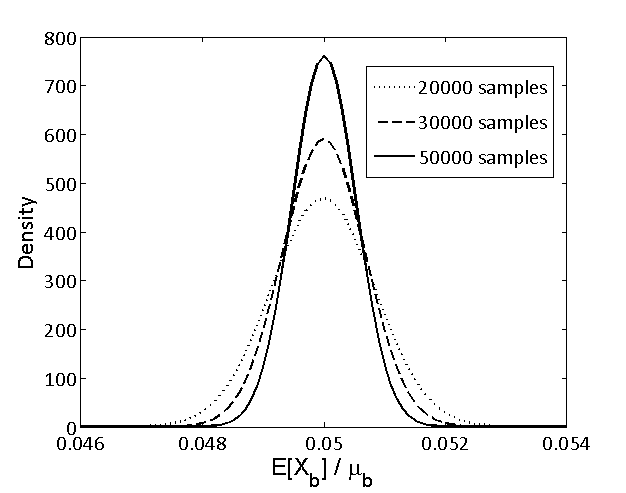
\includegraphics[scale=0.5]{jpdc/figures/figure1paper.png}
\caption{Density functions of the estimation of the percentage of the expected value of $\frac{X_b}{\mu_b}$ according to the Algorithm \ref{alg:simulation} using $N=20000, 30000, 50000$ sample paths}
\label{fig:hist}
\end{figure}

From a parallel point of view, Algorithm~\ref{alg:bestY} can be decomposed into independent tasks, as  there are hardly dependencies in the computation associated to each $Y$. So, the loop ``for" in Algorithm~\ref{alg:bestY} can be executed in parallel. However, the computational burden associated to each $Y$ is different and requires distributing vectors $Y$ among the available processing elements in a balanced way. To do that, an estimation of the workload for each $Y$ is needed.

The workload associated to a feasible timing vector $Y$ (Algorithm~\ref{alg:optimalforY}) can be estimated. In this way the most time-consuming task of this approach (the Monte Carlo simulations) can be taken into account to find the optimal solution. More precisely, the Monte Carlo simulation for an order depends on the length of the replenishment cycle which varies between $1$ and $J$ periods. Following Algorithm \ref{alg:optimalforY}, for cycles in which there is no left inventory, the quantity of product needed  is already known from the so called basic quantities. After that, only one Monte Carlo simulation must be carried out. For any other period, an external function iteratively performs Monte Carlo simulation up to a certain accuracy. With the method used in \cite{GutierrezAlcoba:ICCSA2015}, the number of iterations of Algorithm \ref{alg:simulation} needed to solve the equation line 6 of Algorithm \ref{alg:optimalforY} depends on the accuracy chosen and an average value of $K$ iterations can be assumed. The workload of any vector $Y$ can be taken as the accumulation of Monte Carlo simulations per period that are needed, as sketched in Algorithm~\ref{alg:rankY}.

  \begin{algorithm}[hbt!]
  	\caption{$Rank(Y)$: Workload approximation for $Y$}
  	\label{alg:rankY}
  	\begin{algorithmic}[1]
  	
  		\STATE Generate vectors $A$ and $B$ for $Y$
  		\FOR{$i=1$ \textbf{to} $m$}
  		\STATE $length\_cycle=B_{i-1}-A_{i-1}$;
  		\IF{$A_i=1$ \textbf{or} $length\_cycle=J$} %\# No Invent. 		
  		\STATE $v+=length\_cycle$;
  		%\STATE $floss(Q_i,A_i,A_i+R_i-1)$ \label{optimalforY:line:floss} \#Alg \ref{alg:simulation}
  		\ELSE
  		\STATE $v+=length\_cycle \cdot K$
  		\label{oldalg}
  		%\STATE $Q_i=OrdVal(A_i,A_i+R_i)$ \# Alg~\ref{alg:ordervalue}
  		\ENDIF
  		\ENDFOR
  		\RETURN $v$;
  		\vskip 5pt
  		
  	\end{algorithmic}	
  \end{algorithm}





Now that the parallel decomposition of the problem has been analysed, the details of the implemented approaches are described in the following sections. Section~\ref{sub:MPI-PTHREADS} describes the computational platform and programming interfaces for the MPI-PTHREADS implementation and Section~\ref{sub:GPU} gives the Multi-GPU implementation.  In Section~\ref{SubSec:BinPacking}, the heuristics used to distribute the workload among processing elements are discussed.  Implementations described in~\ref{sub:MPI-PTHREADS} and ~\ref{sub:GPU}  have been carried out on a heterogeneous platform which consists of a multi-GPU cluster (composed of several nodes with multicores and GPU devices). The exploitation of a heterogeneous platform has two main advantages: (1) larger problems can be solved; and (2) it can be done in less runtime.
\begin{itemize}
	\item{MPI-PTHREADS:} obtains the parallelism of the nodes and the multicore processors available in the cluster.
Therefore, programming with POSIX Threads (pthreads~\footnote{\url{https://computing.llnl.gov/tutorials/pthreads/}})  and distributed programming based on Message Passing Interface (MPI) are used~\citep{pthreads,MPI}.
	\item{Multi-GPU:} uses GPUs in order to parallelize the Monte Carlo simulation, which is the most computationally demanding task of the problem. For this, the CUDA~\footnote{\url{https://developer.nvidia.com/cuda-toolkit}}  interface is used. In this case the implementation uses MPI and CUDA.
\end{itemize}



\subsection{MPI-PTHREADS implementation}
\label{sub:MPI-PTHREADS}
Focusing now on the MPI-PTHREADS implementation, parallelism has been exploited on two  levels: at node level (distributed memory) and at multicore level (shared memory).
On one hand, at node level, and thanks to its portability, Message Passing Interface (MPI)~\citep{MPI}
has become a standard for multiple-processor programming of code that runs on a variety of machines.
On the other hand, there are multiple ways of parallelizing routines in shared memory models. One standard library is POSIX threads
(or Pthreads), which supplies a unified set of C routines  facilitating the use of threads in  codes~\citep{pthreads}.

A hybrid parallelization (MPI and Pthreads) of the optimization algorithm for perishable inventory control problem described in Section~3 has been implemented.
At the beginning of Algorithm~\ref{alg:bestY}, the set of timing vectors $Y$ are distributed among cores following the rules of a heuristic designed  for balancing the workload which is discussed in Section~\ref{SubSec:BinPacking}. This MPI-PTHREADS implementation has been tested in a Bullx cluster and obtained results are described in Section~5.



\subsection{Multi-GPU implementation}
\label{sub:GPU}
The Multi-GPU version has been based on the exploitation of several GPUs for the parallelization of the Monte Carlo method, computed by the \emph{flossGPU} function (see Algorithm~\ref{alg:cuda}). In this implementation, each MPI process can open one or two threads and every thread initializes the CUDA interface. Timing vectors $Y$ are distributed among cores in the same way as in the MPI-PTHREADS implementation (following the rules of a heuristic designed  for balancing the workload which is discussed in Section~\ref{SubSec:BinPacking}).
Only Monte Carlo simulations are computed on the GPU, the remaining tasks are computed by the CPU (cores).
  The $N$ sample paths in the Monte Carlo simulation have been implemented to run independently. At the same time, the calculation of the inventory level at each age~(\ref{eq:invWaste}) depends only on the inventory level of the previous period. Then, proceeding by periods, a CUDA kernel is responsible to compute $N$ simulations of the $J$ ages of the inventory in parallel.

In Algorithm~\ref{alg:cuda}, Monte Carlo simulation ($flossGPU$ function) is performed on one or several GPUs.
The external loop simulates the periods, while the inner loop computes $N$ samples on the GPU.
This way, each GPU launches $N$ threads in parallel, computing the same sequence of instructions over
different input data. Thus, the programmer can consider the GPU as a set of SIMT (Single Instruction, Multiple Threads).
Each GPU thread stores its partial computation in the shared memory. To generate the approximation of $X$, one
reduction of the $N$ values computed and stored in shared memory has to be included.
One additional issue has been the optimization of the occupancy on the GPU. The occupancy determines how
well the hardware is kept busy with the goal of hiding
latencies, by switching between active warps, due to memory
operations and paused warps.
Occupancy is closely related
to the thread block size ($BS$) and the number of registers and
shared memory size used by a kernel. Therefore, a good choice
of $BS$ will improve the performance. Experimental results of Section~\ref{Sec:ResultsJPDC} have considered the best $BS$ size (512) to optimize the performance of the GPU code.


Section~\ref{Sec:ResultsJPDC} presents the experimental results of both implementations, MPI-PTHREADS and Multi-GPU.


\begin{algorithm}[bt!]
    \caption{$flossGPU(q,a,b)$: Monte Carlo method for obtaining an approximation of  $E(\textbf{X})$}
    \label{alg:cuda}
    \begin{algorithmic}[1]
        \FOR{$t=a$ \textbf{to} $b$}
        \FOR{$n=1$ \textbf{to} $N$} % \#GPU %(lines 2--5)
        \STATE Update $I_{j,t,n}$, $j=1,\ldots,J$ and $x_{tn}$
        %\STATE $x_b+= \left(d_{b,n}-\sum_{j=1}^{J-1}I_{j,b-1,n}-q\right)^+$;
        \ENDFOR
        \ENDFOR
        \STATE Average loss $X_b=\frac{1}{N}\sum\limits_{n=1}^Nx_{bn}$ approximates $E(\textbf{X})$
        %\STATE $X_b=\frac{x_b}{N}$
        \RETURN $X_b$;
    \end{algorithmic}
\end{algorithm}
%%%%%%%%%%%%%%%%%%%%%%%%%%%%%%%%%%
\subsection{Heuristics for the Bin-Packing problem}
\label{SubSec:BinPacking}


The problem for distributing the workload of Algorithm~\ref{alg:bestY} among processors can be modelled as a Bin packing problem. The Bin-Packing problem is a combinatorial optimization problem (NP-complete) and for the inventory problem it can be described as  follows: Given a set of $L$ independent runs  of the same algorithm with workload  $0< w_i < C$, $i=1,\ldots, L$, for each independent run $i$ of Algorithm  \ref{alg:optimalforY} (the feasible timing order vectors) and a set of $P$ processors (Bins), distribute the runs of the algorithm among the processors $p=1,\ldots,P$ such that the maximum workload assigned to a processor is as low as possible. See~\cite{Garey:1979:CIG:578533} for a general formulation of the Bin-Packing problem.


Due to the hardness of finding optimal solutions for this kind of problems, some heuristics capable of finding acceptable solutions in a reasonable time are usually considered, some of them are based on evolutionary computation, e.g. ~\cite{Blum:2003:MCO:937503.937505}. Here we have tested three heuristics (H1, H2 and H3) which are able to provide approximate solutions to the workload balancing problem.
 These heuristics attempt to distribute the workload $w_i$ equally  over the available cores.
%
\begin{enumerate}
	\item (H1) is based on Round Robin scheduling: Sort $w_i$ from high to low and assign to $p$ following the pattern  $(1,\ldots,P,P,P-1,\ldots,1,1,\ldots)$.
	\item (H2): For $i=1,\ldots,L$ assign $w_i$ to processor $p$ with the lowest gathered workload.
	\item (H3): Similar to heuristic H2, but in this case $w_i$ is sorted previously from high to low values.
\end{enumerate}

To evaluate the heuristics, three  instances called $\Gamma_1$, $\Gamma_2$ and $U$ where generated by taking $L=4000$ weights $w_i$ at random from gamma distributions $\Gamma(10,4)$ and $\Gamma(1,25)$ and from the uniform distribution $U(0,100)$, respectively. Moreover, an instance $\Delta$ was taken from a real workload distribution of the inventory control problem with $T=15$ and $J=3$. Figure \ref{fig:gam} sketches the corresponding distributions.


\begin{figure}[hbt!]
	\centering
	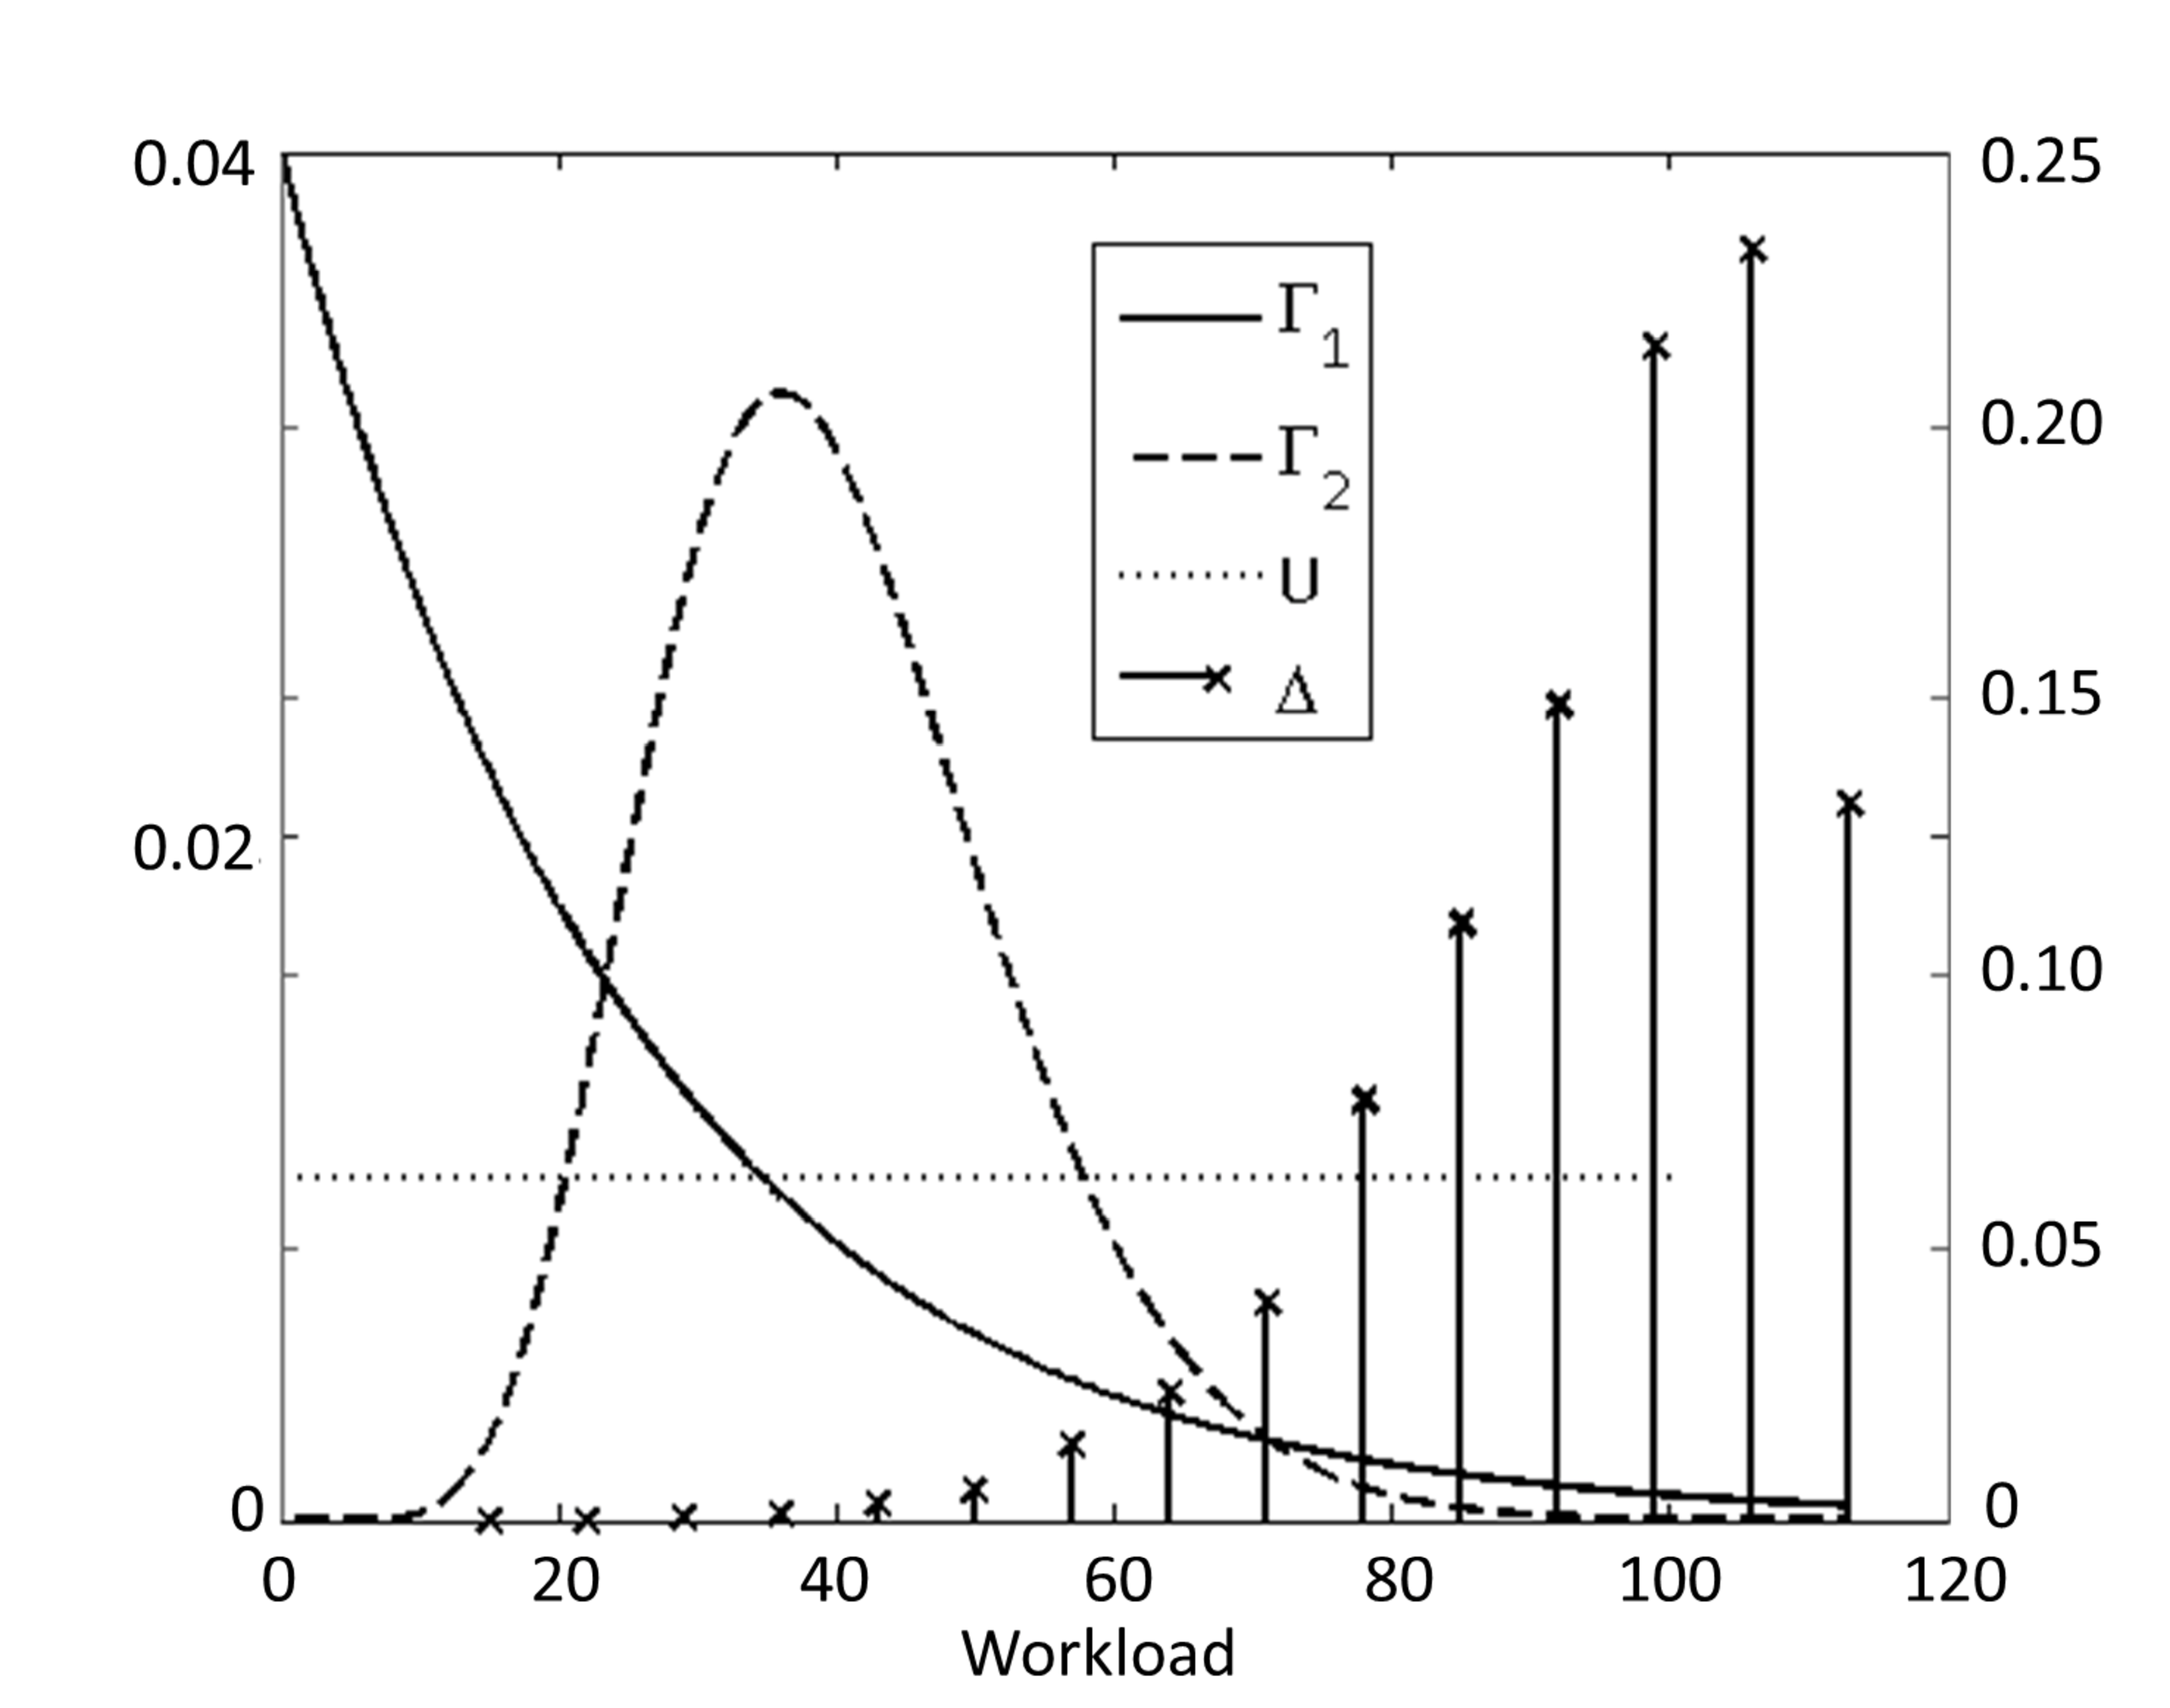
\includegraphics[scale=0.16]{jpdc/figures/figure2.pdf}\\
	\caption{Probability density functions of  $\Gamma (10,4)$, $\Gamma(1,25)$, $U(0,100)$ used to generate the 4000 samples combined with the distribution of the inventory instance, $\Delta$. }
    \label{fig:gam}
\end{figure}

To calculate the workload balancing assigned to each processor, the coefficient of Gini ($G$) \cite{Gini0}
has been used in this work following the examples in~\cite{Gini1,Gini2,Gini3}. This coefficient has been  widely used in economy to measure the degree of inequality and wealth distribution for large populations. The Gini index varies between 0 representing complete equity and 1 if all the wealth (workload) of the population belongs to only one individual (processor)~\cite{Gini0}. Let  $W_p$ be the workload assigned to processor $p$, $p=1,\ldots,P$ sorted in ascending order. The Gini coefficient $G$ is:
%
\begin{equation}
	G= \frac{2\sum\limits_{p=1}^{P} p W_p}{P\sum\limits_{p=1}^{P}W_p}-\frac{P+1}{P}
\end{equation}

Table~\ref{tab:heurperformance} summarizes the behaviour of the heuristics, considering the Gini coefficient ($G$) for the samples (compared to a blind distribution of the workload (HR column)). Clearly, this table shows that heuristic H3 is, at least, better than heuristics H1 and H2 in an order of magnitude, and that a random workload assignment (HR) is at least two orders of magnitude worse than H3 and one for H1 and H2. From the data in Table~\ref{tab:heurperformance}, can be concluded that heuristic H3 presents the best results, being able to balance the workload almost perfectly.

\begin{table}[hbt!]
	
	\caption{Gini coefficient in $10^{-6}$ of the workload distribution of heuristics H1, H2 and H3 versus a random allocation HR.   $P= 8,16,32,64$, weights $w_i$ from  $\Gamma_1$, $\Gamma_2$ and uniform distribution, $\Delta$ is an empirical distribution.}
    \label{tab:heurperformance}
    \centering
    \small
	\begin{tabular}{crrrrr}
		\toprule
    & \multicolumn{1}{c}{$P$} & \multicolumn{1}{c}{H1} &\multicolumn{1}{c}{H2} & \multicolumn{1}{c}{H3} & \multicolumn{1}{c}{HR} \\ \midrule
	\multirow{4}{*}{$\Gamma_1$}	& $8$  &  $130$        	& $480$      	& $12$         & $3700$        \\
		& $16$ &  $250$         	& $1200$      	& $52$         & $7600$        \\
		& $32$ &  $580$          & $2000$      	& $140$         & $13000$        \\
		& $64$ &  $3200$          & $3900$      	& $1500$         & $21000$       \\ \midrule
&\\%%%%%%%%%%%%%%%%%%%%%%%%%%%%%%%%%%%%%%%%%%%%%%%		
	\multirow{4}{*}{$\Gamma_2$} &	$8$  	&  $690$        	& $1000$      	& $19$         & $23000$        \\
		& $16$ 	&  $1200$         	& $2100$      	& $19$         & $39000$        \\
		& $32$ 	&  $3300$          & $4100$      	& $78$         & $61000$        \\
		& $64$ 	&  $8000$          & $7600$      	& $100$         & $79000$         \\	\midrule
&\\%%%%%%%%%%%%%%%%%%%%%%%%%%%%%%%%%%%%%%%%%%%%%%%		
	\multirow{4}{*}{U} &	$8$  	&  $130$        	& $750$      	& $7.4$         & $12000$   \\
		& $16$ 	&  $180$         & $1400$      	& $8.6$         & $18000$        \\
		& $32$ 	&  $220$         & $2400$      	& $39$         & $26000$        \\
		& $64$ 	&  $370$         & $4100$      	& $54$         & $40000$        \\	\midrule		
	\multirow{4}{*}{$\Delta$} &	$8$  	&  $43$        	    & $190$      	& $30$         & $3200$   \\
		& $16$ 	&  $220$         & $460$      	& $230$         & $4500$        \\
		& $32$ 	&  $300$         & $1000$      	& $320$         & $7100$        \\
		& $64$ 	&  $550$         & $2000$      	& $380$         & $9800$        \\	\bottomrule		
	\end{tabular}
\end{table}





\section{Experimental results}
\label{Sec:ResultsJPDC}
For the evaluation of the implementations of Algorithm \ref{alg:bestY} to solve the perishable
inventory control problem, a Bullx cluster composed of eight nodes with a total of 128 cores has been used. In particular,  each node contains two Intel Xeon E5 2650 and a total of 16 cores. The eight nodes are interconnected by a QDR/FDR InfiniBand port embedded on the motherboard. Four of the nodes have two GPUs (total of $2\times4$ NVIDIA Tesla M2070). The main characteristics of the GPUs
are described in Table~\ref{Tab:charGPU}. The experiments have been compiled
with NVIDIA CUDA (6.5 version),  %\blue{
gcc compiler (4.8.1 version) with -O2 as the optimization option and OpenMPI as the MPI library. %}


\begin{table}[hbt!]
    \caption{Characteristics of the GPUs considered for the evaluation.}
    \centering	
    \label{Tab:charGPU}
    \begin{tabular}{rr}
    \toprule
               & Tesla M2070 \\ \midrule
    Peak performance (double prec.) (GFLOPs) &     515 \\
    Peak performance (simple prec.) (GFLOPs) &     1030 \\
    Device memory (GB) &       5.24 \\
    Clock rate (GHz) &        1.2 \\
     Memory bandwidth (GBytes/sec )  &     150 \\
    Multiprocessors &         14 \\
    CUDA cores &        448 \\
    Compute Capability &          2 \\
     DRAM TYPE &      GDDR5 \\ \bottomrule
    \end{tabular}
\end{table}

In order to test the parallel implementations, an inventory control problem of perishable products based on $T=15$ and $J=3$ has been considered.
It comprises a total of $L=5768$ feasible timing vectors $Y$.
For Monte Carlo simulation, $N=200000$ samples are used in Algorithm~\ref{alg:simulation}.

Figure~\ref{fig:MPIPthreadsorder} illustrates the values of the execution time for the MPI-PTHREADS implementation using 1, 2, 4, 8 and 16 threads and 1, 2, 4 and 8 MPI processes. A maximum of eight nodes has been considered. At every node, only one MPI process is executed and the number of Pthreads launched per node varies from 1 to 16 (one thread per physical core). The number of cores $P$ in which the heuristic balances the workload associated to $L$ feasible timing vectors $Y$ of the problem is equal to the number of MPI processes $\times$ the number of threads.




\begin{figure*}[hbt!]
\centering
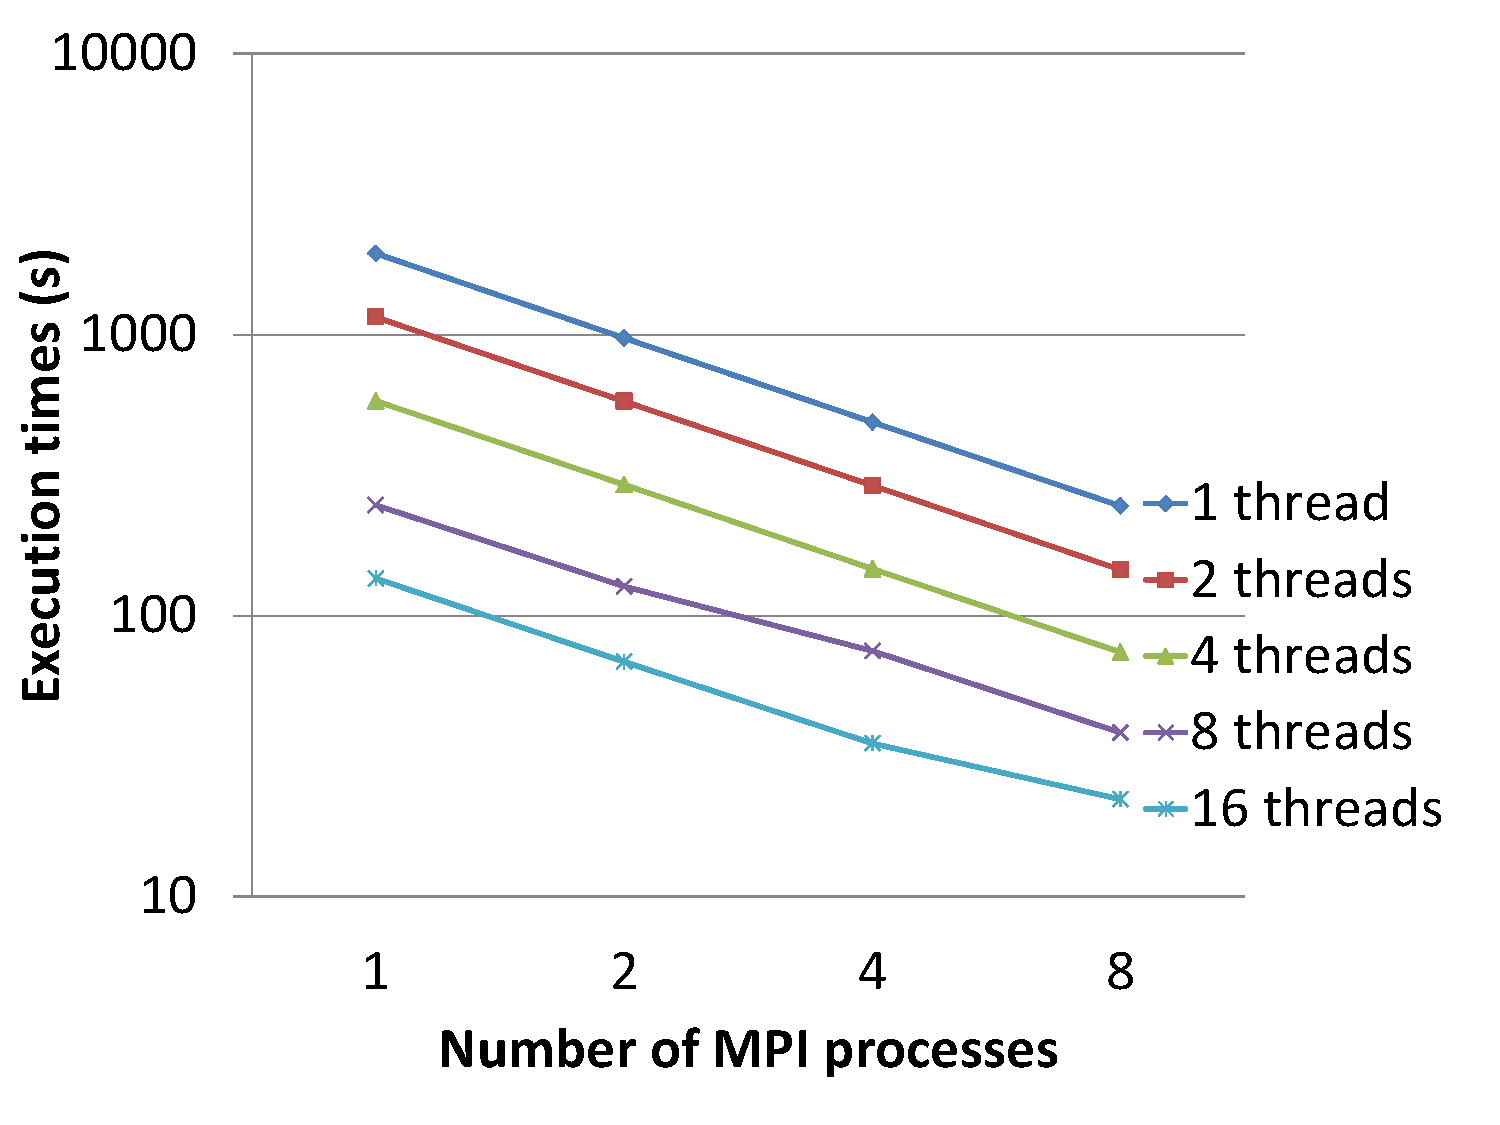
\includegraphics[scale=0.3]{jpdc/figures/MPIPthreadsorder.pdf}
\caption{Executions time, in seconds, of the MPI-PTHREADS implementation using H3 heuristic. }
\label{fig:MPIPthreadsorder}
\end{figure*}


Figure~\ref{fig:SpeedUpMPIPthread} shows the speed up of the MPI-PTHREADS implementation using H3 ranging from $1.7$ for the version with
a single MPI process with 2 threads to $87.5$ for 8 MPI processes with 16 threads each. The performance increases with the number of MPI processes. So, the best
results in terms of performance are obtained for 8 MPI (8 nodes). The Y-axis of the figure highlights how the number of threads in a MPI process affects the total performance of the algorithm. To be more precise, for the same number of MPI processes, duplication of the number of threads (and cores) offers an acceleration factor of nearly $2$.

\begin{figure*}[bt!]
\centering
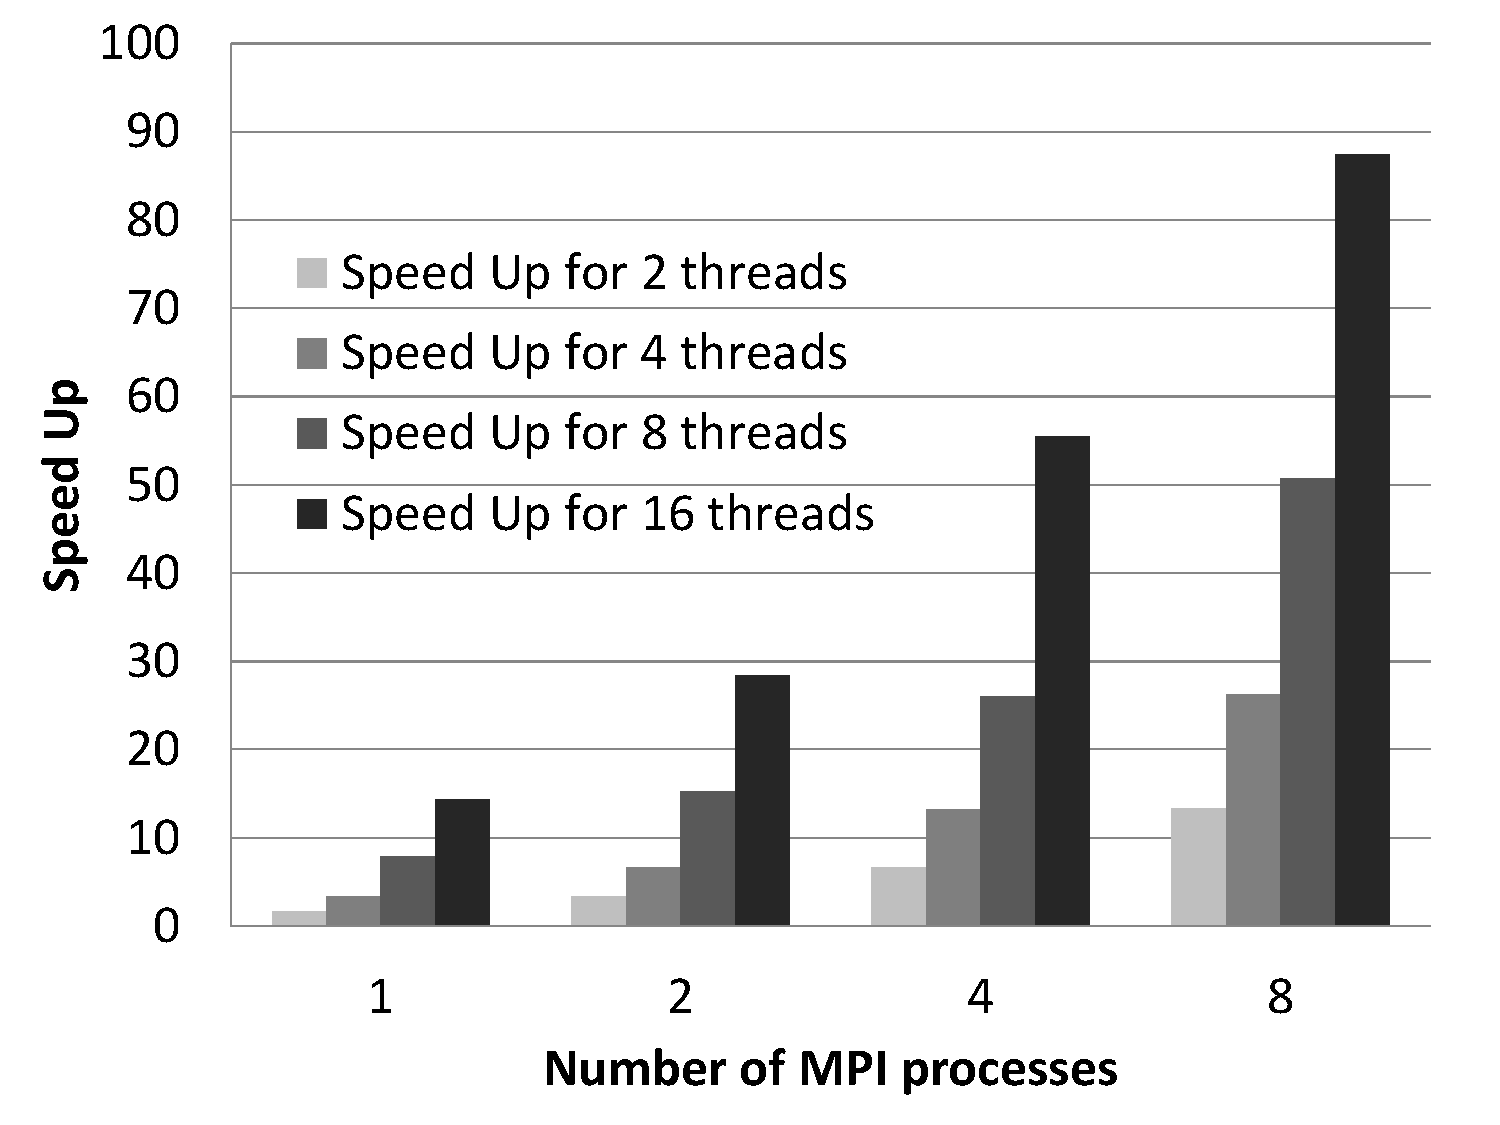
\includegraphics[scale=0.3]{jpdc/figures/SpeedUpMPIPthread.pdf}
\caption{Speed Up of MPI-PTHREADS implementation versus the sequential code, considering H3 heuristic. }
\label{fig:SpeedUpMPIPthread}
\end{figure*}

Table~\ref{tab:GPU} shows the executions time, (in seconds), of the multi-GPU version using 1, 2, 4 and 8 GPUs. Notice that
the information in brackets in the first column identifies the mapping on the cluster of each version. For instance, 6GPU (3MPI, 2 threads) is mapped using 3MPI processes and 2 threads. Moreover,  every thread is associated to one core and one GPU device.
It can be observed that the acceleration factor ranges from $1.99\times$ and $7.72\times$ for 2GPU and 8GPU, respectively. Therefore, the speed up is approximately linear. Column ``\% GPU" represents the percentage of the
total execution time devoted to Monte Carlo function
(\emph{flossGPU} function) using GPU computing, and it can be observed that it is mostly equal to one third of the total runtime.

\begin{table}[!hbt]
	\caption{Execution time, (in seconds), of the multi-GPU version. Total: total execution runtime; GPU (s): runtime (in seconds) of the $flossGPU$ function; $\%$ GPU: percentage of the total execution time devoted to Monte Carlo function ($flossGPU$ function) using GPU computing; AF: acceleration factor of the implementation 1GPU (1MPI, 1 thread) versus the 2GPU, 4GPU, 6GPU, and 8GPU versions. }
	\label{tab:GPU}
	\centering
    \begin{tabular}{rrrrr}
\toprule
              & Total(s) & GPU(s)&$\%$ GPU & AF \\ \midrule
1GPU (1MPI, 1 thread) &185.91 & 56.38 &30.33 & -	\\
2GPU (1MPI, 2 threads) & 93.50	& 28.32 &30.29 &	1.99 \\
4GPU (2MPI, 2 threads) & 44.69	& 14.18 &31.74 &    4.16 \\
6GPU (3MPI, 2 threads) & 33.05	&  9.45 &28.59 &	5.63\\
8GPU (4MPI, 2 threads) & 24.07	&  7.07 &29.39 &	7.72\\
\bottomrule
	\end{tabular}
\end{table}

Comparing  results in Figure~\ref{fig:MPIPthreadsorder}, from the MPI-PTHREADS implementation, to  data in Table~\ref{tab:GPU}, from the multi-GPU version, it can be observed that the runtime when 1MPI and 1 thread are considered for H3 (1941.46s) is much higher (10$\times$ approximately) than the runtime for 1MPI, 1 thread and 1GPU (185.91s). This case illustrates the power of the GPU computation to accelerate this kind of problems. Moreover, focusing our attention on  using 4MPI, 2 threads and 8GPUs of the Table~\ref{tab:GPU}, the total runtime (24.07s) is very similar to the total runtime for 8MPI and 16 threads of the MPI-PTHREADS version (22.19s).
Therefore, in this work, the total runtime of the optimization algorithm for a perishable
inventory control problem has been accelerated by means of two parallel implementations MPI-PTHREADS and multi-GPU. The  results are similar for the configurations with the highest number of nodes, threads and GPUs considered; i.e. for 8MPI and 16 threads (for the MPI-PTHREADS version) and for 4MPI, 2 threads and 8GPU (for the multi-GPU version).


\section{Conclusions}
\label{Sec:Conclusions}
In this chapter two parallel implementations of an optimization algorithm for a perishable
inventory control problem have been studied. A MPI-PTHREADS version
 designed to exploit the parallelism in both multi-core and distributed platforms; and a multi-GPU version which
uses GPU computing to accelerate the most computationally intensive task (Monte Carlo simulation).
The MPI-PTHREADS parallelization using a static workload balancing based on H3 heuristic has shown a good scalability.
The results have shown that MPI-PTHREADS implementation has a good scalability when increasing both the number of processes (nodes) and threads (cores). Therefore, using 8 MPI processes and 16 threads the performance has been increased in a factor of $87$ versus the sequential code.
Finally, parallelization of the Monte Carlo function (\emph{GPUfloss} function) with 8 GPUs speeds up running time with a factor of $81$ versus the sequential code. It has been shown that both parallel implementations, MPI-PTHREADS and multi-GPU, can considerably accelerate the optimization algorithm for the perishable
inventory control problem studied in this work.

 Implemented software for the perishable inventory control on heterogeneous platforms is freely available through the following website: \url{https://sites.google.com/site/hpcoptimizationproblems/inventory-problem}.

%\section*{Acknowledgement}
%Alejandro G. Alcoba is a fellow of the Spanish FPI programme. This paper has been supported by The Spanish Ministry (TIN2015-66680) and Junta de Andalucia (P11-TIC-7176), in part financed by the European Regional Development Fund (ERDF).

%\section*{References}

%\bibliography{bibInventory}

%\end{document} 
\clearemptydoublepage	
\include{IJPR/IJPR}
\clearemptydoublepage
%\documentclass[]{article}
%\documentclass[procedia]{easychair}
%
%% This provides the \BibTeX macro
%\usepackage{doc}
%\usepackage{makeidx}
%\usepackage[utf8]{inputenc}
%
%
% \usepackage{graphicx}
%%% or use the epsfig package if you prefer to use the old commands
%\usepackage{epsfig}
%
%\usepackage{amsmath}
%%\usepackage{algorithm}
%\usepackage{t1enc}
%%% The amssymb package provides various useful mathematical symbols
%\usepackage{amssymb}
%%% The amsthm package provides extended theorem environments
%\usepackage{amsthm}
%\usepackage{hyperref}
%\newcommand{\blue}{\textcolor{blue}}
%\newcommand{\rcomment}[1]{\hfill {\it\bf \small #1}}
%\newcommand\ceil[1]{\lceil#1\rceil}
%\newcommand{\tb}{\hspace{2ex}}
%%\newcommand{\rcomment}[1]{\hfill {\it \small #1}}
%\renewcommand{\epsilon}{\varepsilon}
%
%\newtheoremstyle{example}{\topsep}{\topsep}%
%     {}%         Body font
%     {}%         Indent amount (empty = no indent, \parindent = para indent)
%     {\bfseries}% Thm head font
%     {}%        Punctuation after thm head
%     {\newline}%     Space after thm head (\newline = linebreak)
%     {\thmname{#1}\thmnumber{ #2}\thmnote{ #3}}%         Thm head spec
%
%\theoremstyle{example}
%\newtheorem{example}{Example}
%
%
%
%\usepackage{color}
%\usepackage{algorithm}
%\usepackage{algorithmic}
%\usepackage[usenames,dvipsnames]{xcolor}
%\usepackage{comment}
%%\algrenewcommand{\algorithmiccomment}[1]{\hfill$\blacktriangleright$ #1}
%%\newcommand{\blue}{\textcolor{blue}}
%%\newcommand{\emt}{\textcolor{blue}}
%\newcommand{\red}{\textcolor{red}}
%\newcommand{\green}{\textcolor{green}}
%
%
%
%\def\procediaConference{ICCS 2017}
% 
%\title{A model for optimal fleet composition of vessels for offshore wind farm maintenance}
%\titlerunning{On fleet composition for OWF maintenance}
%
%\author{
%	Alejandro Gutierrez-Alcoba\inst{1}\thanks{Alejandro Gutierrez-Alcoba is a fellow of the Spanish FPI programme, granted by the Ministry of Economy, Industry and Competitiveness. This paper has been supported by The Spanish Ministry (TIN2015-66680) and Seneca Foundation (19241/PI/14) of the Murcia region, in part financed by the European Regional Development Fund (ERDF).}%\thanks{Designed and implemented the class style}
%	\and
%	Gloria Ortega\inst{2}%\thanks{Did numerous tests and provided a lot of suggestions}
%	\and
%	Eligius M.T. Hendrix\inst{1}
%	\and
%%	Dag Haugland\inst{3}
%%	\and
%	Elin E. Halvorsen-Weare\inst{3}
%	\and
%	Dag Haugland \inst{4}
%}
%
%\institute{
%	Computer Arquitecture Dpt., Universidad de M\'alaga,
%	Málaga, Spain\\
%	\email{agutierrez@ac.uma.es;eligius@uma.es}
%	\and
%    Informatics Dpt.,
%	University of Almería, Agrifood Campus of Int. Excell. (ceiA3),
%	Almería, Spain\\
%	\email{gloriaortega@ual.es}\\
%	\and
%	Department of Maritime Transport Systems, MARINTEK,
%	%P.O. Box 4125 Valentinlyst, NO-7450
%	Trondheim, Norway\\
%	\email{elin.halvorsen-weare@marintek.sintef.no }\\
%	\and
%	Department of Informatics, University of Bergen,
%	P.O. Box 7803, 5020 Bergen,
%	Norway\\
%	\email{dag.haugland@uib.no}\\
%}
%\authorrunning{Gutierrez-Alcoba, et al.}
%
%\begin{document}	
%%opening
%\maketitle
%%\author{Authors}
%\keywords{Offshore Wind Farms, Decision Support System, Fleet composition, Maintenance planning}
%
%
%%\date{}
%
%
%\begin{abstract}
%We present a discrete optimisation model that chooses an optimal fleet of vessels to support maintenance operations at Offshore Wind Farms (OFWs). The model is presented as a bi-level problem. On the first (tactical) level, decisions are made on the fleet composition for a certain time horizon. On the second (operational) level, the fleet is used to optimise the schedule of operations needed at the OWF, given events of failures and weather conditions.
%\end{abstract}
%\begin{keyword}
%fleet composition \sep maintenance \sep wind farm

%\end{keyword}
\newcommand\ceil[1]{\lceil#1\rceil}
\chapter{A model for optimal fleet composition of vessels for offshore wind farm maintenance} % top level followed by section, subsection
\label{Chap:iccs2017}

\ifpdf
    \graphicspath{{X/figures/PNG/}{X/figures/PDF/}{X/figures/}}
\else
    \graphicspath{{X/figures/EPS/}{X/figures/}}
\fi


\section{Introduction}


The offshore wind energy industry is expected to continue its growth tendency in the near future. The European Wind Energy Association expects in its Central Scenario by 2030 a total installed capacity of 66 GW of offshore wind in the UE \cite{WES2030}.


Offshore wind farms (OWFs) are large scale infrastructures, requiring large fleets able to perform operations and maintenance (O\&M) activities in the installed turbines, constituting one of the major costs of running an OWF installation. The fleet makes the installations  dependent on non-renewable energy resources. Therefore, optimising the efficiency of the resources used for the O\&M activities of an OWF becomes extremely important in order to make them economically viable and to reduce CO2 emissions.
%Conference paper cite: \cite{Stalhane2016}


%\section{Literature Review}
%\label{litreview}

Recent deterministic and stochastic model formulations for vessel composition and maintenance optimization  can be found in \cite{Gundegjerde2015} and \cite{HALVORSENWEARE2013}. A recent literature review on DSS for OWF's is given by \cite{hofmannrev}.
%
In~\cite{EJOR2016}, a model for maintenance routing
and scheduling at offshore wind farms based on the Dantzig-Wolfe decomposition method has been implemented.
In that work, a mixed integer linear program is solved for each subset of turbines to generate all  feasible routes and maintenance schedules for the vessels for each period.
The routes take several constraints into account, such as weather conditions, the availability of vessels,
and the number of technicians available at the operation and maintenance base.
%
In~\cite{Stalhane2016357}, a two-stage stochastic programming model is presented to determine a cost-optimal fleet size and mix for
O\&M activities at offshore wind farms for the total expected lifetime of the OWF. For that, the study considers time periods fixed to three months.




This chapter presents a model for the use of vessels in OWF maintenance. The lower level decisions are based on a two shift a day period, that takes weather conditions into account. Although breakdown events and weather circumstances (wind) are stochastic events, they are handled in the model by a scenario approach in a deterministic way to come to a (lower) estimate of the expected costs of the fleet composition plan. This deterministic approach generates a lower bound for costs in the the operational stage and facilitates finding the optimal fleet of vessels for a long time horizon using small time periods (small bucket approach). The model considers a set of types of maintenance activities that are needed to be performed in an OWF and selects a set of bases and vessel types and finds, for each scenario, a schedule of operations for the planning horizon minimising costs. The challenge for this type of models is that the number of integer and binary variables becomes large complicating the solution time. 

The rest of this chapter is organised as follows. Section \ref{sec:problemdescriptionICCS} describes  the properties of the problem of operating an OWF and selecting a fleet to support their maintenance activities in detail. Section \ref{sec:mathematicalformulationICCS} sets the mathematical formulation of the model, describing the objective function and the constraints associated to the tactical and the operational decisions. Section \ref{sec:computationalstudyICCS} presents the computational study that has been carried out to test the model. Finally, Section \ref{sec:conclusionICCS} concludes this chapter.


\section{Problem definition}
\label{sec:problemdescriptionICCS}

This section describes the maintenance planning problem to be solved. The decision problem is related to a fleet of vessels and the maintenance activities that are supported at an offshore wind farm during a planning horizon. The aim is to find an optimal fleet of vessels and a collection of maintenance activities to be performed on the wind turbines. The model is based on the more extensive model description of a fleet size and mix decision model in~\cite{Elin}. That model contains a more detailed description of the operational scheduling dealing with each individual action. The model in the current paper also takes a small bucket approach of scheduling, distinguishing periods of 12 hours, but aggregates to a number of activities in each period.

Maintenance activities are divided into \emph{preventive} and \emph{corrective} ones. Each activity type has an estimated duration, cost, and requires a number of maintenance technicians. Preventive maintenance activities are meant to prevent failures and prolong the lifetime of wind turbines. Examples of preventive activity types include: visual inspection, changing of consumables, oil sampling, and tightening of bolts \cite{obdam}. Corrective maintenance activities are needed to repair wind turbines that have suffered a breakdown.

Preventive activities to be scheduled are determined by the decision maker beforehand, who fixes a number of preventive activities of each type that need to be performed throughout the planning horizon. Corrective activities are only needed after a specific failure occurs in a wind turbine. There is a downtime cost associated to the lack of electricity production in turbines during the execution of a maintenance activity and while a breakdown continues. %Hence the importance of performing corrective activities as failures occur, or performing preventive maintenance activities when the wind is lower, trying to avoid periods in which the turbines can produce more electricity

Preventive maintenance activities should be planned somewhere within the time horizon. The corrective activity types are generated beforehand. The planner is confronted in each scenario with failure types. There is one-to-one correspondence between failures types and corrective activity types. The instrument available to the planner for handling activities is a \emph{bundle}. It includes the description of a trip by a vessel $v$ from base $k$ that contributes possibly to one or more activities.


To perform these maintenance activities, a fleet of vessels is needed. Vessel types have properties such as the type of maintenance activities they can perform, capacity for technicians, a yearly depreciation cost over the planning horizon and the speed they can sail.  Every vessel is associated with a base, from which they travel to the wind farm to perform maintenance activities. Each base has a certain vessel capacity, a capacity to accommodate technicians, an associated cost and coordinates which provide their distance to the wind farm. 



The decision maker selects a number of candidate bases that can be used and a number of vessels of each type associated to them, subject to the particular conditions of each base. Each vessel type is able to support a particular set of bundles, considering their properties. A bundle consists of one or several maintenance activities to be performed at the OWF that fits in a shift.  Some activity types do not require the vessel to be present at the turbine. In that case it is possible to perform several activities in parallel in a single time period. It is irrelevant whether  a bundle contains activities that run in parallel or sequentially, as long as they meet the time constraints of a period and the vessel type can accommodate enough technicians to perform the activities. Moreover, some activity types take longer than the time available in a single shift. These long activities are split into smaller chunks. The model keeps track of how much time has been invested in each activity type to control when they are finished. If a long activity is initiated in one period, it does not necessarily have to be continued in the following. However, for corrective activities, downtime costs are incurred for the next shifts until the activity is finished and the failure in the turbine is solved.

In the model in the current chapter, decisions are taken on two levels: the first level decides which bases to use and which vessels should be available during the time horizon period under consideration. On the second level, the optimal operation decisions for each scenario are determined including which maintenance activities to support by which vessel type in every period of the planning horizon and for every possible scenario. Scenarios
consist of weather conditions preventing use of vessels for maintenance, availability of personnel and the possible failures of turbines that require corrective maintenance activity types.



\section{Mathematical formulation}
\label{sec:mathematicalformulationICCS}

In this section, we present the two-level deterministic optimisation model to generate and evaluate the optimal fleet of vessels to perform maintenance activities at offshore wind farms. The following symbols are used to describe the mathematical optimisation model.


%USE THIS PARAGRAPH LATER: Implicitly, the individual activity schedule follows from a FIFO approach, where the first activity that has been started is the first to be ended.

%\scalebox{1}{
\begin{tabular}{ll}
	\multicolumn{2}{l}{Sets}\\
	%K
	%V
	$\mathcal{K}$ 				& 	Set of bases \\
	$\mathcal{V}_k$ 				& 	Set of vessel types at base $k$ \\
	$\mathcal{S}$ 				& 	Set of scenarios \\	
%	$\mathcal{T}$ 				& 	Set of time periods in the planning horizon \\	
	$\Gamma$ 					&	Set of maintenance activity types \\
	$\mathcal{NP}$				&	Subset of planned preventive maintenance activity types, \\
	                            & $\mathcal{NP}\subset\Gamma$ \\
	$\mathcal{NC}$				&	Subset of corrective maintenance activity types, $\mathcal{NC}\subset\Gamma$ \\
	$\mathcal{P}$				&	Set of all possible bundles\\
	$\mathcal{P}_{kv}$			&	Set of possible bundles for a vessel of type $v$ from base $k$\\
%\end{tabular}



%\begin{tabular}{ll}
	\\
  \multicolumn{2}{l}{Parameters}\\
  
	$T$ & Number of periods (days) in the planning horizon\\
	$F_{k}$ 	&	Fixed cost per year of operating base $k$\\
	$G_{v}$ 	&	Charter or depreciation cost for using vessel type $v$ over the \\
				&    complete horizon\\
	$D_{st}$	&	Loss due to downtime of performing a maintenance  $s$\\ 
				& activity in scenario in period $t$ \\
	$C_{kvp}$ 	&	Cost of executing bundle $p$ from base $b$ and a vessel of type\\
				& $v$\\
	$CP_i$ 		&	Penalty cost for not executing a preventive maintenance\\
				& activity of type $i\in \mathcal{NP}$\\
	%$NI_{i}$ 		&	Number of hours required by preventive maintenance activity $i$\\
	$N_{i}$ 		&	\parbox[t]{10cm}{Number of hours required by maintenance activity of type}\\
					& $i\in \Gamma$ during the time horizon\\
	$PP_{i}$ 		&	Number of planned preventive maintenance activities of type\\
					& $i\in \mathcal{NP}$\\	
	$H_{i t}$ 		&	\parbox[t]{10cm}{Expected hourly downtime cost for a preventive  activity of type $i\in \mathcal{NP}$ in period $t$}\\
	$M_{k}$ 		&	Number of maintenance technicians available at base $k\in K$\\
					& in each shift\\
	$MP_{p}$ 		&	\parbox[t]{10cm}{Required maintenance technician personnel to elaborate}\\
					& bundle $p$\\
	$Q_{kv}$ 		& \parbox[t]{10cm}{Maximum number of vessels type $v$ that can operate from}\\
					& base $k$\\
	$B_{i}$ &	Hours spent on an activity of type $i$ in one shift\\
	$A_{ip}$ 		&	Number of activities of type $i$ in bundle $p$\\
	$P_s$ 		&	Probability of scenario $s$\\
	$Y_{its}$ 	& 	\parbox[t]{10cm}{Number of failures of type $i\in\mathcal{NC}$ accumulated in periods}\\
				& $1,\ldots,t$ in scenario $s$.
	\\
\end{tabular}
%}

\begin{tabular}{ll}
	\\
	\multicolumn{2}{l}{Tactical decision variables}\\
	$y_{k} \in \{0,1\}$ 	& Equal to 1 if base $k$ is used, 0 otherwise\\
	$x_{kv} \in\{0,\ldots,Q_{kv}\}$ &	Number of vessels type $v$ operated from base $k$\\
	\\
	%
\end{tabular}	

\begin{tabular}{ll}	
	\multicolumn{2}{l}{Operational decision variables}\\

	%$\delta_k$	&	Equal to 1 if base $k\in K$ is used, 0 otherwise\\
	$w_{its}\in\mathbb{Z}^+$	&	\parbox[t]{10cm}{Number of corrective maintenance activities of type  $i \in\mathcal{NC}$ supported during period $t$ in scenario $s$}\\
	$q_{its} \in\mathbb{Z}^+$	&	\parbox[t]{10cm}{Number of preventive maintenance activities of type $i \in \mathcal{NP}$ supported during period $t$ in scenario $s$}\\
	$u_{pts}\in\mathbb{Z}^+$ &	\parbox[t]{10cm}{Number of vessels executing bundle $p$ during period $t$ in scenario $s$}\\
	$r_{its}\in\mathbb{Z}^+$	&	\parbox[t]{10cm}{Number of corrective maintenance activities of type  $i \in\mathcal{NC}$ that are not (yet) completed in scenario $s$ in period $t$}\\
	$z_{i s}\in\mathbb{Z}^+$	&	\parbox[t]{10cm}{Number of preventive maintenance activities of type $i \in \mathcal{NP}$ not completed in scenario $s$ at the end of the time horizon}\\
								\\	
\end{tabular}

In order to solve the model, it is necessary to predefine the bounds on the variables as sharp as possible. Sharp bounds facilitate the pre-solving operations of an LP solver that filter out those variables that have a value of zero and those constraints that are not binding.


\begin{align}
\label{eq:bound1ICCS}
  0 \leq x_{kv} \leq Q_{kv},				&\quad	\forall k,v\\
\label{eq:bound2ICCS}
  0 \leq u_{pts} \leq \sum\limits_{k\in\mathcal{K}} \sum\limits_{v\in\mathcal{V}_k} Q_{kv} &\quad \forall p,s,t  \\
\label{eq:bound3ICCS}
0 \leq w_{its} \leq \sum\limits_{k} \sum\limits_{v} Q_{kv}\max\limits_{p\in \mathcal{P}_{kv}}A_{ip} 	&\quad i \in \mathcal{NP} \\
\label{eq:bound4ICCS}  	
0 \leq q_{its} \leq \sum\limits_{k} \sum\limits_{v} Q_{kv}\max\limits_{p\in \mathcal{P}_{kv}}A_{ip} 	&\quad i \in \mathcal{NC} \\
\label{eq:bound5ICCS}
  0 \leq r_{i st}\leq Y_{i ts} &\quad	\forall i\in\mathcal{NC},s,t\\
\label{eq:bound6ICCS}
   0 \leq z_{i s}\leq PP_{i} &\quad	\forall i\in\mathcal{NP},s
\end{align}



The value of parameter $Q_{kv}$ is an upper bound on the number of vessels that can be used from each base. Therefore, the number of bundles that can be performed in a shift for a particular scenario is bounded by the total capacity of vessels for the considered bases. The number of preventive activities not performed at the end of the horizon is bounded by the total number of planned preventive activities $PP_i$. The number of corrective activities not finished at a certain shift is bounded above by the total occurrences of failures $Y_{its}$ thus far.


\subsection{Objective function}

The objective is to minimise the fixed costs of operating the bases and the charter cost of the selected vessels, the costs of all the bundles executed throughout the planning horizon, the downtime costs associated with the execution of maintenance activities or persistent failures and the penalty costs of preventive and corrective activity types that are not finished within the planning horizon:
%
\begin{align}
\label{eq:objfunICCS}
 \min & 	\sum\limits_{k\in \mathcal{K}} F_k y_k  %1
	      + \sum\limits_{k\in \mathcal{K}}\sum\limits_{v\in\mathcal{V}_k} G_v x_{kv} %2
	      + \sum\limits_{s\in\mathcal{S}} P_{s} \left(\sum\limits_{k\in\mathcal{K}} \sum\limits_{v\in\mathcal{V}_k} \sum\limits_{p\in\mathcal{P}_{kv}} \sum\limits_{t=1}^T C_{kvp}u_{pts}\right) +\\ \nonumber
	    & \sum\limits_{s\in\mathcal{S}} P_{s} \left(\sum\limits_{i\in \mathcal{NP}}  \sum\limits_{t=1}^TH_{i t}B_{i}q_{its}
+ \sum\limits_{i \in\mathcal{NC}} \sum\limits_{t=1}^T D_{st} r_{i st} +  \sum\limits_{i \in\mathcal{NP}} CP_i z_{i s} + \sum\limits_{i \in\mathcal{NC}} CP_i r_{isT}\right)%6
\end{align}
%
The first two terms of the objective function (\ref{eq:objfunICCS}) cover the costs for the tactical decisions: which bases and vessels will be used. The first term refers to the fixed costs for operating the chosen bases during the complete planning horizon. The second defines the charter cost for the available fleet of vessels during the complete planning horizon.

The following terms cover the expected operational costs of the model. Therefore, the cost of each scenario is  multiplied by its probability. The third term of the objective function (\ref{eq:objfunICCS}) determines the cost of operating the bundles during the planning horizon. Terms four and five describe the downtime costs of preventive and corrective activity types, respectively. While the downtime costs for preventive activity types are only incurred while an activity is taking place on a turbine, downtime for corrective activity types initiate from the period the breakdown occurs and continues until the period in which it is finished. The last two terms are related to the penalty costs. Term six is the penalty incurred for the preventive maintenance activity types that are not performed within the planning horizon while term seven is the penalty for corrective ones.



\subsection{Constraints for tactical decisions}

There is only one constraint on the tactical decisions:
%
\begin{align}
\label{eq:const1:maxVkfromKICCS}
  x_{kv} \leq Q_{kv}y_{k}  	&	&	\forall k, v
\end{align}
%
The constraint describes the usual relation that base $k$ should be in use, if one wants to station vessels there. One can add limitations on which bases should be used. The tactical decision directly intervenes in the possibilities of the operational planning.

\subsection{Constraints on operational decisions}
Constraints on the operational decisions are expressed in terms of the following inequalities:
\begin{align}
\label{eq:const1ICCS}
  \sum\limits_{p\in \mathcal{P}_{kv}} u_{pts}\le x_{kv}, 			&\quad		\forall k,v,t,s\\
  \label{eq:const4ICCS}
  \sum\limits_{v\in V_k}\sum\limits_{p\in \mathcal{P}_{kv}} MP_{p}u_{pts} \leq M_{k},				&\quad	\forall k,s,t\\
  \label{eq:const5ICCS}
   \sum\limits_{p}^{\mathcal{P}} A_{ip}u_{pts} - q_{its}\geq 0,				&\quad	i\in \mathcal{NP}, \forall s, t\\
   \label{eq:const6ICCS}
   \sum\limits_{p}^{\mathcal{P}} A_{ip}u_{pts} - w_{its}\geq 0,				&\quad	i\in \mathcal{NC}, \forall s, t\\
\label{eq:const:rwICCS}
  \frac{N_{i}}{B_{i}}(Y_{its}-r_{its}) \leq  \sum\limits_{\tau=1}^t \sum\limits_{p \in \mathcal{P}} w_{i\tau s}\leq \ceil{\frac{N_{i}}{B_{i}} Y_{its}}, 		 &\quad	\forall s,i \in\mathcal{NC}, t=1,\ldots,T\\
\label{eq:const3ICCS}
   N_{i}z_{is}+ \sum\limits_{t=1}^T B_{i}q_{its}\ge N_{i}PP_{i}, 		&\quad	\forall i \in \mathcal{NP},s
\end{align}
%
Constraint \eqref{eq:const1ICCS} limits the operations on the availability of sufficient vessels at each base.
Constraint \eqref{eq:const4ICCS} describes the limits on operations due to available personnel.
Constraints \eqref{eq:const5ICCS} and \eqref{eq:const6ICCS} link the assignment of the activities depending on the the planned bundles and availability of vessels.
Constraint \eqref{eq:const:rwICCS} keeps track of the number of corrective activities not finished (lower bound) and assures that the number of activities performed for a single type does not exceed the number of turbines having that failure type (upper bound). One should round up the number $\frac{N_i}{B_i}Y_{its}$. If this is not done, the constraint cannot allow the last chunk of a large activity type to be performed until another failure of the same type occurs and consequently $Y_{its}$ increases.
Finally, constraint \eqref{eq:const3ICCS} describes the number of preventive activities for each type that are not finished in scenario $s$.

Implicitly, constraints \eqref{eq:const:rwICCS} and \eqref{eq:const3ICCS} imply that the individual activity schedule follows from a FIFO approach for preventive and corrective activity types, where the first activity that has been started is the first to be ended.



%Constraints \eqref{eq:constsomany} and \eqref{eq:only1fori} guarantee that in one shift at most one operation is contributing to each activity.

\section{Computational study}
\label{sec:computationalstudyICCS}

Discussing the validity of the model, it is worthwhile to mention that in principle the lower level operational planning cost provides a lower bound for the incurred cost due to failures and downtime. By formulating the operational activities in a one-shot model, in principle all the scenario is known beforehand and earlier activities can be planned based on knowledge of failures that will occur later. This makes the planning in principle cheaper than what is possible in reality. On the other hand, due to the  nature of the variable $r_{its}$, there is a tension in the optimal outcome to start repairing a failure as soon as possible by a corrective activity. We will investigate the amount of underestimation for specific realistic data in future work confronting the optimal MILP outcome of the lower level for scenarios with a simulated more realistic behaviour.

The complete bi-level model described in Section \ref{sec:mathematicalformulationICCS} has been implemented using the GAMS interface \cite{gams} and has been solved using the CPLEX solver, setting the optimality gap at 10\%. The tests have been carried out on a (DELL Optiplex 390) computer with an Intel i3-2110,3.3 GHz processor, (8 GB) RAM running in Windows. The instances have been generated in Matlab using cost data from \cite{obdam}.

\subsection{Description of a case study}
\label{subsec:casestudy}
In this section we describe the case study that has been considered to conduct experiments to test the model presented in this chapter.

We consider an OWF consisting of 125 turbines. The planning horizon is one year and the periods represent 12 hour shifts and include a return trip from the base the vessel is located to the OWF and a bundle of activities. In practical terms there are 730 periods. There are three available bases $B_1,B_2,B_3$ around the OWF, each of which can accommodate up to 36 technicians and they are located at 110, 61  and 86 kilometres respectively from the OWF. The cost of using each of them, for the entire time horizon is 2, 6 and 7 million monetary units (mu) respectively.

Four types of vessels are considered: $V_1,V_2,V_3,V_4$. Each base has space to allow two vessels of type $V_1$, two of type $V_2$, four of type $V_3$ and one of type $V_4$. Vessel type $V_4$ is able to accommodate up to 30 technicians, while the rest has space for only 12. The cost of having a vessel during the whole planning horizon for vessel types $V_1$, $V_2$, $V_3$ and $V_4$ is, respectively, 122,4000, 2,500,000, 750,000 and 7,200,000 mu. Vessel types $V_1$ and $V_2$ can travel at a speed of 20 knots, while vessel types $V_3$ and $V_4$ can travel at 40 knots. In practical terms this means that vessel types $V_1$ and $V_2$ require about 5.94, 3.3 and 4.64 hours to perform a return trip between bases $B_1$, $B_2$ and $B_3$ respectively while vessel types $V_3$ and $V_4$ would require half of that time, allowing more time to perform activities in each shift.

\begin{table}[]
	\centering
	\caption{Possible efficient bundles that can be performed from each base-vessel combination}
	\label{tab:bundles}
	\begin{tabular}{llll}
		$k$  & $v$ &  $\mathcal{P}$                                                                                                                  &  \\
		$B_1$ & $V_1$       & $\{(0,0,4,0)\}$                                                                                                                  &  \\
		$B_1$ & $V_2$       & $\{(0,0,4,0)\}$                                                                                                                  &  \\
		$B_1$ & $V_3$       & $\{(3,0,0,0),(0,2,0,0),(0,0,4,0),(0,0,0,1)\}$                                                                                    &  \\
		$B_1$ & $V_4$       & $\{(6,0,0,0),(3,3,0,0),(2,2,2,0),(3,0,3,0),(0,3,3,0),(0,0,6,0),$\\
			  & 			& $(0,0,0,1)\}$                                                      										 &  \\
		$B_2$ & $V_1$       & $\{(3,0,0,0),(0,2,0,0),(0,0,4,0),(0,0,0,1)\}$                                                                                    &  \\
		$B_2$ & $V_2$       & $\{(3,0,0,0),(0,2,0,0),(0,0,4,0),(0,0,0,1)\}$                                                                                    &  \\
		$B_2$ & $V_3$       & $\{(3,0,0,0),(0,2,0,0),(0,0,4,0),(0,0,0,1)\}$                                                                                    &  \\
		$B_2$ & $V_4$       & $\{(6,0,0,0),(3,3,0,0),(0,6,0,0),(2,2,2,0),(3,0,3,0),(0,3,3,0),$\\
			  &				& $(0,0,6,0),(0,0,0,1)\}$ &  \\
		$B_3$ & $V_1$       & $\{(3,0,0,0),(0,0,4,0),(0,0,0,1)\}$                                                                                              &  \\
		$B_3$ & $V_2$       & $\{(3,0,0,0),(0,0,4,0),(0,0,0,1)\}$                                                                                              &  \\
		$B_3$ & $V_3$       & $\{(3,0,0,0),(0,2,0,0),(0,0,4,0),(0,0,0,1)\}$                                                                                    &  \\
		$B_3$ & $V_4$       & $\{(6,0,0,0),(3,3,0,0),(2,2,2,0),(3,0,3,0),(0,3,3,0),$\\
			  &				& $(0,0,6,0),(0,0,0,1)\}$                                                      &
	\end{tabular}
\end{table}

There are two preventive activity types $A_1,A_2$ and two corrective activity types $A_3, A_4$. All vessel types are able to perform all the activity types considered. Activity type $A_4$ requires the vessel supporting the operation to be present at the turbine while the activity is performed, whereas activity types $A_1,A_2,A_3$ can be run in parallel. The vessel drops a group of technicians at each turbine that is going to be supported during the shift. The time required to perform activity types $A_1$, $A_2$, $A_3$ and $A_4$ is 60 , 100 , 3 and 7.5 hours respectively. The maximum time per period and turbine that a group of technicians can support an activity type is 6 hours. Consequently, only activities of type $A_3$ can be performed in a single period. The penalty cost for not executing a preventive activity type is 10 million mu. For corrective activities of type $A_3$ the cost is 50,000 mu, and for type $A_4$, the penalty cost rises to 500,000 mu.

A series of bundles of activities that each vessel type can perform from each base is presented in Table \ref{tab:bundles}. Bases closer to the OWF and faster vessel types are able to spend more time at the OWF during a 12 hours period, facilitating more activities to take place in a single bundle and a larger set of different bundles. The cost of a bundle depends on the type of vessel used and the base of departure (see Table \ref{tab:costbundle}), but not on the performed activity.

For our case study, there are 125 planned activities of type $A_1$ and 60 of type $A_2$. The number of corrective activity types corresponds to the number of failures of the turbines and depends on the scenario. A scenario consists of the events of the failures of the turbines and the wind speed at the OWF for every period. Failures that require corrective activity types $A_3$ and $A_4$ follow a binomial distribution. The rate of failures for a corrective activity of type $A_3$ is 5 times per turbine per year, and 3 times per turbine a year for failures that require an activity of type $A_4$. Wind conditions are not simulated. Instead, they are taken from historical weather data. For each scenario, a report file containing a year of wind speed data of the OWF area is picked randomly.




\begin{table}[]
\centering
\caption{Bundle costs for each base-vessel combination. Bundles with the same base-vessel combination have the same costs.}
\label{tab:costbundle}
\begin{tabular}{lll|lll|lll}
$k$  & $v$ & $C_{kvp}$ & $k$  & $v$ & $C_{kvp}$ & $k$  & $v$ & $C_{kvp}$  \\
$B_1$ & $V_1$       & 2310    & $B_2$ & $V_1$       & 1281    & $B_3$ & $V_1$       & 1806    \\
$B_1$ & $V_2$       & 2310    & $B_2$ & $V_2$       & 1281    & $B_3$ & $V_2$       & 1806    \\
$B_1$ & $V_3$       & 3300    & $B_2$ & $V_3$       & 1830    & $B_3$ & $V_3$       & 2580    \\
$B_1$ & $V_4$       & 6600    & $B_2$ & $V_4$       & 3660    & $B_3$ & $V_4$       & 5160
\end{tabular}
\end{table}

\subsection{Optimal fleet of vessels}

The case study presented in \ref{subsec:casestudy} of the bi-level model with only 3 scenarios consists of an  MILP problem with about 50,000  constraints and more than 300,000 variables. The pre-solve operation using the data of the instance, eliminates many rows and columns, but leaves a relatively complex problem to be solved. In fact, that instance exceeds the 24 hour limit of executing time. For two scenarios, the optimal fleet given by the solver was to operate three vessels of type $V_3$ from base $B_1$. The optimal solution value given by the solver was 10,321,000 mu.


The costs associated to the tactical level add up to 4,250,000 mu; that is the cost of maintaining base $B_1$ and operating the selected vessels. The execution of patterns incurred another 5,227,200 mu, leaving the rest 843,800 mu corresponding to downtime costs, incurred during breakdowns and maintenance activities.
In terms of electricity production this amounts to the equivalent of losing the potential of about one turbine during the time horizon.

\subsection{Performance of the model}
For testing the performance of the model, we have run the case described in \ref{subsec:casestudy}, varying the number of scenarios and the time horizon. We have considered the different instances of the case study problem taking one, two and three scenarios. For the time horizon 90 , 180 and 365 days of planning have been considered. The number of constraints and variables for each case is laid out in Table \ref{tab:constnvar}. The execution times for each of theses instances is presented in Table \ref{tab:time}, expressed in minutes. These figures increase rapidly in the number of considered scenarios and the time horizon. The instance consisting on 365 days for the time horizon (730 periods) and three scenarios did not reach the set optimality gap in 24 hours of execution.

\begin{table}[h!]
\centering
\caption{Number of constraints and variables for different instances of the model varying the number of scenarios ($\left|\mathcal{S}\right|=1,2,3$) and the time horizon ($T=90,180,365$)}
\label{tab:constnvar}
\begin{tabular}{l|cccccc}
$\left|\mathcal{S}\right|$ \textbackslash T & \multicolumn{2}{c}{90}                                    & \multicolumn{2}{c}{180}                                   & \multicolumn{2}{c}{365}                                   \\
                                            & \multicolumn{1}{l}{N const.} & \multicolumn{1}{l}{N var.} & \multicolumn{1}{l}{N const.} & \multicolumn{1}{l}{N var.} & \multicolumn{1}{l}{N const.} & \multicolumn{1}{l}{N var.} \\ \hline
1                                           &  4,162                         & 25,767                      & 8,304                         & 51,507                      & 16,814                        &  104,417                     \\
2                                           &  8,304                         & 51,509                      & 16,584                        &  102,989                     & 33,602                        &  208,809                     \\
3                                           & 12,440                        & 77,251                      & 24,864                        &  154,471                     & 50,396                        & 313,201                    
\end{tabular}
\end{table}



\begin{table}[h!]
\centering
\caption{Execution times, in minutes, for different instances of the model varying the number of scenarios ($\left|\mathcal{S}\right|=1,2,3$) and the time horizon ($T=90,180,365$)}
\label{tab:time}
\begin{tabular}{c|ccc}
$\left|\mathcal{S}\right|$ \textbackslash T                           & \multicolumn{1}{l}{90} & \multicolumn{1}{l}{180} & \multicolumn{1}{l}{365} \\ \hline
1 & 2                       & 5                        & 49                          \\
2 & 3.5                        & 12                          & 203                          \\
3 & 11                        & 57                          & n/a                        
\end{tabular}
\end{table}

\section{Conclusion}
\label{sec:conclusionICCS}
This chapter presents a discrete optimisation model for selecting an optimal fleet of vessels to support maintenance operations at OFW's. To determine the optimal fleet and their operations, the model has been presented as a bi-level problem. At the first (tactical) level, the model determines the optimal fleet. At the second (operational) level, it schedules operations needed at the OWF throughout the time horizon. A case study has been developed to test the performance of the model, analysing the optimal fleet of vessels given by the solver. The performance tests show the complexity of the presented model for large time horizons.

Future work includes considering weather circumstances in the model that may limit the use of vessels for maintenance operations, such as wind speed, wave height and visibility. The generation of bundles for base-vessel configurations will be revisited, in order to automatise it. One of our questions is how to solve the model presented in a more efficient way, for a large number of scenarios. Moreover, we will investigate the amount of underestimation for specific realistic data confronting the optimal MILP outcome of the lower operational level for scenarios with a simulated more realistic behaviour. 


%\bibliographystyle{plain}
%\bibliography{bibOWF}


\clearemptydoublepage	

\chapter{On offshore wind farm maintenance scheduling for decision support on vessel fleet composition }
\label{Chap:ejor}
\ifpdf
\graphicspath{{X/figures/PNG/}{X/figures/PDF/}{X/figures/}}
\else
\graphicspath{{X/figures/EPS/}{X/figures/}}
\fi

The following chapter is an extension of Chapter \ref{Chap:iccs2017}.
%\begin{abstract}
%Maintenance costs account for a large part of the total cost of an offshore wind farm. Several models have been presented in the literature to optimize the fleet composition of the required vessels to support maintenance tasks. We provide a mixed integer linear programming (MILP) description of such a model, where on the higher level, the fleet composition is decided and on the lower level the maintenance operations are scheduled for a set of weather and breakdown scenarios. A drawback of deciding a perfect information schedule for the coming year is that in fact, the weather outcomes and breakdowns are not known in advance. Consequently, given a fleet composition, its corresponding maintenance costs are underestimated compared to what can be realised in practice under incomplete information. Therefore, we present several heuristics that simulate the practical scheduling and may provide a better cost estimate. The latter method is used to evaluate a fleet composition based on available information and it is compared with the MILP solution based on complete information.
%You did not make a greedy heuristic for fleet composition. Just a herustic scheduler for maintenance operations. You do not compare generated fleet, but you evaluate two fleet compositions. The outcomes of the procedure are compared to the underestimated fleet composition of the complete information MILP approach for a practical instance.
%\end{abstract}

%\begin{keyword}
%Scheduling \sep Offshore Wind Farm \sep Heuristic \sep Fleet composition \sep Maintenance planning
%\end{keyword}

%\end{frontmatter}


\section{Introduction}


The offshore wind energy industry is expected to continue its growth tendency in the near future. The European Wind Energy Association expects in its Central Scenario by 2030 a total installed capacity of 66 GW of offshore wind in the EU \cite{WES2030}.
%
Offshore wind farms (OWFs) are large scale infrastructures, requiring a large fleet of vessels able to perform operations and maintenance (O\&M) tasks on the installed turbines. The O\&M constitutes a large part of the costs of running an OWF installation, being up to one third of the OWF costs \cite{Snyder20091567}. Moreover, the fleet makes the installations  depend on non-renewable energy resources. Therefore, optimising the efficiency of the resources used for the O\&M tasks of an OWF becomes extremely important in order to make them economically viable and to reduce CO2 emissions.

Recent deterministic and stochastic model formulations for vessel composition and  optimization of maintenance operations at OWF's can be found in \cite{Gundegjerde2015} and \cite{HALVORSENWEARE2013}. A recent literature review on DSS for OWF's is given by \cite{hofmannrev}.
%
In~\cite{LijuanDai,EJOR2016} and \cite{STALHANE201592}, a model for maintenance routing and scheduling at offshore wind farms based on the Dantzig-Wolfe decomposition method has been implemented.
In that work, a mixed integer linear program is solved for each subset of turbines to generate all  feasible routes and maintenance schedules for the vessels for each period.
The routes take several constraints into account, such as weather conditions, the availability of vessels and the number of technicians available at the operation and maintenance base.
%
In~\cite{Stalhane2016357}, a two-stage stochastic programming model is presented to determine a cost-optimal fleet size and mix for O\&M tasks at offshore wind farms for the total expected lifetime of the OWF. For that, the study considers time periods fixed to three months.

The basis of our investigation is a scenario based MILP model which like the models in \cite{HALVORSENWEARE2013} and \cite{Stalhane2016357} decides on the vessel fleet composition. All these models evaluate the value of the vessel fleet composition and base selection based on scheduling with perfect information; the weather conditions and breakdowns happening during a scenario of a year are known beforehand. The research question in the current paper is whether the vessel fleet composition may be affected when maintenance scheduling is done in a heuristic way following a practical decision rule given the available information at the time of maintenance scheduling.

We investigate this question in the following way. Section \ref{sec:problemdescriptionEJOR} describes the practical decision problem of operating an OWF and selecting a fleet to support its maintenance tasks. Section \ref{sec:mathematicalformulation} describes an MILP model, which simultaneously determines the maintenance scheduling as well as the fleet composition. In Section \ref{sec:heuristic}, a heuristic for the operational stage of the model is presented. Section \ref{sec:computationalstudyEJOR} presents a computational study used to compare the outcomes of both procedures. Finally, Section \ref{sec:conclusion} summarises our findings.


\section{Problem definition}
\label{sec:problemdescriptionEJOR}

This section describes the maintenance planning problem related to a fleet of vessels for an offshore wind farm during a planning horizon, based on a more extensive model of fleet size and mix decisions in~\cite{Elin}. The aim is to find an optimal fleet of vessels and a collection of maintenance tasks to be performed on the wind turbines. That model contains a detailed description of the operational scheduling dealing with each individual action. Our vision also distinguishes  periods (shifts) of 12 hours, but aggregates a number of tasks in each period (shift).


\emph{Preventive} as \emph{corrective} maintenance tasks are considered.
Preventive maintenance tasks are meant to prevent failures and prolong the lifetime of wind turbines. Examples include visual inspection, changing of consumables, oil sampling, and tightening of bolts \cite{obdam}. Corrective maintenance tasks are needed to repair broken down wind turbines. There is a one-to-one correspondence between failure types and corrective task types.


The number of necessary preventive tasks of each type to be performed is predefined at the beginning of the year. Corrective tasks are only needed after a specific failure occurs in a wind turbine. The planner is confronted in each scenario with failures occurring dynamically. There is a downtime cost associated to the lack of electricity production in turbines during the execution of a maintenance task. Downtime costs are also considered for broken down turbines, incurred for the shifts from diagnose until reparation.




To perform the maintenance tasks, a fleet of vessels is needed. Vessel types have properties such as the type of maintenance tasks they can perform, capacity for transferring technicians, a depreciation cost over the planning horizon, a sailing speed and a threshold for wind speed and wave height that prevents to transfer technicians to the turbines or sailing if they are exceeded. Every vessel is associated to a base, from which it travels to the wind farm to perform maintenance tasks. Each base has a certain vessel capacity, a capacity to accommodate technicians, an associated cost and coordinates which provide its distance to the wind farm.

The decision problem includes a number of candidate bases that can be used and a number of vessel types associated to them. Each vessel type is able to support a particular set of patterns, from the base they are associated with. A pattern consists of one or several maintenance tasks to be performed at the OWF that fits in a shift, including the time it takes the vessel type to perform a round trip visiting the OWF from their base. For each shift the available vessels are able to perform a single pattern of the possible ones that are associated to their type and their base. Some patterns from different vessel types and associated to different bases might be virtually the same, containing the same list of tasks to be performed during the shift. Their cost and time required may vary, considering the speed of the vessel or the distance from their base to the OWF.  Some task types do not require the vessel to be present at the turbine. This facilitates performing several tasks in parallel in a single time shift. It is irrelevant whether  a pattern contains tasks that run in parallel or sequentially, as long as they meet the time constraints of a shift and the vessel type can accommodate enough technicians to perform the tasks. Moreover, some task types take longer than the time available in a single shift. These long tasks are split into smaller parts that fit with the duration of the shifts. If a long task is initiated in one shift, it does not necessarily have to be continued in the following. However, for corrective tasks, downtime costs are incurred for all shifts until the task is finished and the failure in the turbine has been repaired.

Decisions actually take place on two levels: the first (tactical) level decides which bases to use and which vessels should be available during the planning horizon period under consideration. The second (operational) level schedules operations  including which patterns to support by which available vessel in every shift of the planning horizon. The random events the planner is confronted with consist of weather conditions preventing use of vessels for maintenance and the possible failures of turbines that require corrective maintenance tasks.



\section{MILP model description}
\label{sec:mathematicalformulation}

Like in the models of \cite{HALVORSENWEARE2013} and \cite{Stalhane2016357},
%Elin says this are not the papers....
 the tactical level decisions are evaluated based on a scenario approach, where the planner has perfect information to schedule the operational maintenance tasks. The following symbols are used to describe the mathematical optimisation model.


%\scalebox{1}{
\begin{tabular}{ll}
	\multicolumn{2}{l}{Sets}\\
	%K
	%V
	$\mathcal{K}$ 				& 	Set of bases \\
	$\mathcal{V}_k$ 				& 	Set of vessel types at base $k$ \\
	$\mathcal{S}$ 				& 	Set of scenarios \\	
%	$\mathcal{T}$ 				& 	Set of time periods in the planning horizon \\	
	$\mathcal{T}_{vs}$			&	Set of shifts not suitable for sailing due to weather limitations \\
								&	for vessel type $v$ during scenario $s$\\
	$\Gamma$ 					&	Set of maintenance task types \\
	$\mathcal{NP}$				&	Subset of planned preventive maintenance task types, $\mathcal{NP}\subset\Gamma$ \\
	$\mathcal{NC}$				&	Subset of corrective maintenance task types, $\mathcal{NC}\subset\Gamma$ \\
	$\mathcal{P}$				&	Set of all possible patterns\\
	$\mathcal{P}_{kv}$			&	\parbox[t]{10cm}{Set of possible patterns for a vessel of type $v$ operating from base $k$}\\
\end{tabular}



\begin{tabular}{ll}
	\\
  \multicolumn{2}{l}{Parameters}\\
	$T$ & Number of shifts in the planning horizon\\
	$F_{k}$ 	&	Fixed cost per year of operating base $k$\\
	$G_{v}$ 	&	\parbox[t]{10cm}{Charter or depreciation cost for using a vessel of type $v$ over the complete planning horizon}\\
	$D_{st}$	&	\parbox[t]{10cm}{Income loss due to downtime of performing a maintenance task in scenario $s$ in shift $t$} \\
	$H_{ts}$ 		&	\parbox[t]{10cm}{Hourly income loss due to downtime of performing a maintenance task in scenario $s$ in shift $t$}\\
	%This is actually D_st / 12, being 12 in this case the number of hours of a shift
	$C_{p}$ 	&	\parbox[t]{10cm}{Cost of executing pattern $p\in \mathcal{P}_{kv}$ from base $k$ and a vessel of type $v$ }\\
	$CP_i$ 	&	\parbox[t]{10cm}{Penalty cost for not executing a preventive maintenance task of type $i\in \mathcal{NP}$}\\
%	\end{tabular}
	
%\begin{tabular}{ll}
	%\\
  \multicolumn{2}{l}{}\\	
	%$NI_{i}$ 		&	Number of hours required by preventive maintenance task $i$\\
	$N_{i}$ 		&	\parbox[t]{10cm}{Number of hours required to execute maintenance task of type $i\in \Gamma$ during the planning horizon}\\
	$PP_{i}$ 		&	\parbox[t]{10cm}{Number of planned preventive maintenance tasks of type $i\in \mathcal{NP}$}\\	
	$M_{k}$ 		&	\parbox[t]{10cm}{Number of maintenance technicians available at base $k\in K$ in each shift}\\
	$MP_{p}$ 		&	\parbox[t]{10cm}{Required number of maintenance technician personnel to execute pattern $p$} \\
	$Q_{kv}$ 	&	\parbox[t]{10cm}{Maximum number of vessels of type $v$ that can operate from base $k$}\\
	$B_{i}$ &	\parbox[t]{10cm}{Hours spent on a task of type $i$ in one shift, being $B_i \leq N_i$}\\
	$A_{ip}$ 		&	\parbox[t]{10cm}{Number of tasks of type $i$ in pattern $p$}\\
	$P_s$ 		&	Probability of scenario $s$\\
	$Y_{its}$ 	& 	\parbox[t]{10cm}{Number of failures of type $i\in\mathcal{NC}$ accumulated in shifts $1,\ldots,t$ in scenario $s$}.
	\\
%\end{tabular}
%}

%\begin{tabular}{ll}
	\\
	\multicolumn{2}{l}{Tactical decision variables}\\
	$y_{k} \in \{0,1\}$ 	& Equal to 1 if base $k$ is used, 0 otherwise\\
	$x_{kv} \in\{0,\ldots,Q_{kv}\}$ &	Number of vessels of type $v$ operated from base $k$\\
	\\
	%
%\end{tabular}	

%\begin{tabular}{ll}	
	\multicolumn{2}{l}{Operational decision variables}\\
	$w_{its}\in\mathbb{Z}^+$	&	\parbox[t]{9.5cm}{Number of corrective maintenance tasks of type  $i \in\mathcal{NC}$ supported during shift $t$ in scenario $s$}\\
	$q_{its} \in\mathbb{Z}^+$	&	\parbox[t]{9.5cm}{Number of preventive maintenance tasks of type $i \in \mathcal{NP}$ supported during shift $t$ in scenario $s$}\\
	$u_{pts}\in\mathbb{Z}^+$ &	\parbox[t]{9.5cm}{Number of vessels executing pattern $p$ during shift $t$ in scenario $s$}\\
	$\bar{w}_{its}\in\mathbb{Z}^+$	&	\parbox[t]{9.5cm}{Number of corrective maintenance tasks of type  $i \in\mathcal{NC}$ that are not (yet) completed in scenario $s$ in shift $t$}\\
	$\bar{q}_{i s}\in\mathbb{Z}^+$	&	\parbox[t]{9.5cm}{Number of preventive maintenance tasks of type $i \in \mathcal{NP}$ not completed in scenario $s$ at the end of the planning horizon}  \\
								\\	
\end{tabular}

In order to solve the model, the bounds on the variables should be set as sharp as possible to facilitate pre-solving operations of an LP solver that filters out those variables that have a value of zero and those constraints that are not binding. We define the following bounds:


\begin{align}
\label{eq:bound1}
  0 \leq x_{kv} \leq Q_{kv},				&\quad	\forall k,v\\
\label{eq:bound2}
  0 \leq u_{pts} \leq \sum\limits_{k\in\mathcal{K}} \sum\limits_{v\in\mathcal{V}_k} Q_{kv} &\quad \forall p,s,t  \\
\label{eq:bound3}
0 \leq w_{its} \leq \sum\limits_{k\in\mathcal{K}} \sum\limits_{v\in\mathcal{V}_k} Q_{kv}\max\limits_{p\in \mathcal{P}_{kv}}A_{ip} 	&\quad \forall i \in \mathcal{NP}, \forall t,s\\
\label{eq:bound4}  	
0 \leq q_{its} \leq \sum\limits_{k\in\mathcal{K}} \sum\limits_{v\in\mathcal{V}_k} Q_{kv}\max\limits_{p\in \mathcal{P}_{kv}}A_{ip} 	&\quad \forall i \in \mathcal{NC}, \forall t,s\\
\label{eq:bound5}
  0 \leq \bar{w}_{its}\leq Y_{i ts} &\quad	\forall i\in\mathcal{NC}, \forall t,s\\
\label{eq:bound6}
   0 \leq \bar{q}{is}\leq PP_{i} &\quad	\forall i\in\mathcal{NP}, \forall s
\end{align}



The value of parameter $Q_{kv}$ is an upper bound on the number of vessels that can be used from each base. Therefore, the number of patterns that can be performed in a shift for a particular scenario is bounded by the total capacity of vessels for the considered bases. The number of corrective tasks not finished at a certain shift is bounded above by the total occurrences of failures $Y_{its}$ thus far.
The number of preventive tasks not performed at the end of the horizon is bounded by the total number of planned preventive tasks $PP_i$.


\subsection{Objective function}

The objective is to minimise the fixed costs of operating the bases and the charter cost of the selected vessels, the costs of all performed patterns throughout the planning horizon, the downtime costs associated with the running maintenance tasks or persistent failures and the penalty costs of preventive and corrective task types that are not finished within the planning horizon:
%
\begin{align}
\label{eq:objfun}
 \min  	\sum\limits_{k\in \mathcal{K}} F_k y_k  %1
	      + \sum\limits_{k\in \mathcal{K}}\sum\limits_{v\in\mathcal{V}_k} G_v x_{kv} %2
	      + \sum\limits_{s\in\mathcal{S}} P_{s} \left(\sum\limits_{k\in\mathcal{K}} \sum\limits_{v\in\mathcal{V}_k} \sum\limits_{p\in\mathcal{P}_{kv}} \sum\limits_{t=1}^T C_{p}u_{pts}\right) +\\ \nonumber
	     \sum\limits_{s\in\mathcal{S}} P_{s} \left(\sum\limits_{i\in \mathcal{NP}}  \sum\limits_{t=1}^TH_{ts}B_{i}q_{its}
+ \sum\limits_{i \in\mathcal{NC}} \sum\limits_{t=1}^T D_{st} \bar{w}_{its} +  \sum\limits_{i \in\mathcal{NP}} CP_i \bar{q}_{is} + \sum\limits_{i \in\mathcal{NC}} CP_i \bar{w}_{iTs}\right)
\end{align}
%
The first two terms of the objective function (\ref{eq:objfun}) cover the costs for the tactical decisions: cost of bases and vessels. The first term refers to the fixed costs for operating the chosen base(s) during the  planning horizon. The second defines the charter costs for the available fleet of vessels during the  planning horizon.

The following terms cover the expected operational costs of the model. Therefore, the cost of each scenario is  multiplied by its probability. The third term of the objective function (\ref{eq:objfun}) determines the cost of operating the patterns during the planning horizon. Terms four and five describe the downtime costs of preventive and corrective task types, respectively. While the downtime costs for preventive task types are only incurred while a task is taking place on a turbine, downtime for corrective task types initiate from the moment the breakdown occurs and continues until the shift in which it has been repaired. The last two terms are related to penalty costs. Term six is the penalty incurred for the preventive maintenance task types that are not performed within the planning horizon while term seven is the penalty for not finishing all corrective tasks.



\subsection{Constraints for tactical decisions}

There is only one constraint on the tactical level describing the usual relation that base $k$ should be in use, if one wants to station vessels there, and set the bounds of the maximum number of each vessel type for each base.

\begin{align}
\label{eq:const1:maxVkfromK}
  x_{kv} \leq Q_{kv}y_{k}  	&	&	\forall k, v
\end{align}
%
 The tactical decision directly influences the possibilities of the operational planning. A larger fleet allows to perform more patterns each shift.

\subsection{Constraints on operational decisions}
Constraints on the operational level are given by the following inequalities:
\begin{align}
\label{eq:const1}
  %\sum\limits_{\{p|k_p=k,v_p=v\}} u_{pts}\le x_{kv}, 			&\quad		\forall k,v,t,s\\
  \sum\limits_{p\in \mathcal{P}_{kv}} u_{pts}\le x_{kv}, 			&\quad		\forall k,v,t,s\\
  \label{eq:const4}
  %\sum\limits_{\{p|k_p=k\}} MP_{p}u_{pts} \leq M_{k},				&\quad	\forall k,s,t\\
  \sum\limits_{v\in V_k}\sum\limits_{p\in \mathcal{P}_{kv}} MP_{p}u_{pts} \leq M_{k},				&\quad	\forall k,s,t\\
  \label{eq:const5}
   \sum\limits_{p\in \mathcal{P}_{kv}} A_{ip}u_{pts} - q_{its}\geq 0,				&\quad	\forall i\in \mathcal{NP}, \forall k,v,s, t\\
   \label{eq:const6}
   \sum\limits_{p\in \mathcal{P}_{kv}} A_{ip}u_{pts} - w_{its}\geq 0,				&\quad	\forall i\in \mathcal{NC}, \forall k,v,s, t\\
\label{eq:const:rw}
  \frac{N_{i}}{B_{i}}(Y_{its}-\bar{w}_{its}) \leq  \sum\limits_{\tau=1}^t  w_{i\tau s}\leq \ceil{\frac{N_{i}}{B_{i}} Y_{its}}, 		 &\quad	\forall i \in\mathcal{NC}, \forall s,t\\
    %\frac{N_{i}}{B_{i}}(Y_{its}-\bar{w}_{its}) \leq  \sum\limits_{\tau=1}^t \sum\limits_{p \in \mathcal{P}} w_{i\tau s}\leq \ceil{\frac{N_{i}}{B_{i}} Y_{its}}, 		 &\quad	\forall i \in\mathcal{NC}, \forall s,t\\
\label{eq:const3}
   N_{i}\bar{q}_{is}+ \sum\limits_{t=1}^T B_{i}q_{its}\ge N_{i}PP_{i}, 		&\quad \forall i \in \mathcal{NP}, \forall s\\
\label{eq:constweather}
   	u_{pts}=0, &\quad \forall p\in \mathcal{P}, \forall t \in \mathcal{T}_{vs}, \forall s
\end{align}
%
Constraint \eqref{eq:const1} bounds operations on the availability of sufficient vessels at each base. Each available vessel has the potential to contribute performing one of its possible patterns each shift.
Constraint \eqref{eq:const4} limits operations due to available personnel at the bases.
Constraints \eqref{eq:const5} and \eqref{eq:const6} link the assignment of individual tasks to planned patterns and availability of vessels, for preventive and corrective types respectively. It is necessary to keep track of not finished corrective tasks every shift, as the turbines affected incur downtime costs until they are fixed.
The lower bound of constraint \eqref{eq:const:rw} keeps track of the number of not finished corrective tasks (breakdowns). The planner cannot complete more corrective tasks than the ones present at the OWF every shift. The upper bound ensures that the number of single type tasks does not exceed the number of broken down turbines caused by the same failure type. Also, a single corrective task of type $i$  contributes with $B_i$ hours during a shift, while $N_i\geq B_i$ hours are needed to complete the a complete task of type $i$. Therefore, the number $\frac{N_i}{B_i}Y_{its}$ should be rounded up allowing the last part of a large task to be performed. Otherwise, in case just one corrective task of type $i$ is needed and $B_i\nmid N_i$, the task could not be finished until another failure of type $i$ occurs, increasing$Y_{its}$. For preventive tasks it is only necessary to check the number of not performed tasks at the end of the time horizon. Constraint \eqref{eq:const3} keeps track of the number of preventive tasks for each type that have not been finalised in scenario $s$.

Implicitly, constraints \eqref{eq:const:rw} and \eqref{eq:const3} imply that the individual task schedule follows from a FIFO approach for preventive and corrective task types, where the first task that has been started is the first to be ended. Such assumption is needed: if each task was treated as an independent task the model would become intractable for small instances. Finally, constraint \ref{eq:constweather} prevents patterns to be performed during shifts in which the weather conditions exceed the threshold of wind speed or wave height for the vessel type used to execute the pattern.



%Constraints \eqref{eq:constsomany} and \eqref{eq:only1fori} guarantee that in one shift at most one operation is contributing to each task.
\subsection{Generating columns (bundles and patterns) for the model}
\label{subsec:buildpatterns}
%\subsection{Generation of bundles and patterns}
The basic decisions of the scheduler of the maintenance operations are based on feasible patterns, previously crafted by the decision maker. This section describes an automatic procedure to generate the feasible maintenance patterns for every base and vessel type combination. A recursive algorithm can be used for this task, considering constraints such as the number of technicians needed or the time limitations to complete the pattern.

As sketched in Section \ref{sec:problemdescriptionEJOR}, some task types do not require the vessel to be present at the turbine during the operation such that these types can be run in parallel. We will indicate them by the set $\Gamma p_v$. Therefore, the generation of columns is based on a two-step procedure. First, we generate the feasible set of bundles of tasks that include only task types from $\Gamma p_v$ that can be run in parallel using a recursive procedure described in Algorithm \ref{alg:buildbundle}. In the second step, we combine these bundles with the non-parallel task types in $\Gamma n_v$ to create the final set of patterns.


A bundle $b$ is specified as a quadruple (List, Time, Cost, Tech) specifying the list of activites, the time to execute it, the cost and the number of technicians required, respectively. Each task in List is performed at a different turbine and they are run in parallel. During the execution of a bundle, the vessel docks to the first turbine, offloads the task materials and technicians required and then moves to another turbine until all the tasks are started. When finished, the vessel recollects the technicians and returns to base. The duration (Time) of a bundle consists of the set up time (setupTime$_i$) for its tasks and the docking time (docktime$_v$) at each turbine when dropping off and when picking up the technicians. With respect to the time $B_i$ spent on a single task, we have to keep in mind they are run in parallel. The procedure has to take into account the number of technicians Tech$_v$ allowed on vessel $v$ and the number of hours TMX$_v$ it may stay at the Offshore wind farm. Finally, the cost of a task Cost$_i$ and the number of required technicians Tech$_i$ is updated.

%Elin said to put the alg. after explaining all the parameters etc...

\begin{algorithm}[h]
	\caption{build\_bundle(Bundle $b$, Vessel $v$)}
	\label{alg:buildbundle}
	\begin{algorithmic}
		%\REQUIRE say here
		%\ENSURE say here
		\medskip
		\FOR {all $i\in \Gamma p_v$}
		\STATE $T_{vi}$= 2*dockTime$_v$+setupTime$_i$;
		%\IF {$v$ not needed in turbine for task $i$\green{This if is not needed after declaring $\Gamma p_v$. Parallel task and not needed in turbine ar equivalent}}
		\STATE temp\_time=max(Time+$T_{vi}$,$B_i$+$T_{vi}$)
		\STATE temp\_cost= Cost+Cost$_i$
		\STATE temp\_tech= Tech + Tech$_i$
		\STATE temp\_list by adding $i$ to List
		\IF {temp\_time $\leq$ TMX$_v$ and temp\_tech $\leq$ Tech$_v$}
		\STATE define new bundle $\hat b$=(temp\_list,temp\_time,temp\_cost,temp\_tech)
		\STATE $\mathcal{B}_v= \mathcal{B}_v\cup \{\hat b\}$
		\STATE build\_bundle($\hat b$,$v$)
		%\ENDIF
		%\ENDIF
		\ENDIF
		\ENDFOR	
	\end{algorithmic}
\end{algorithm}
The procedure, starting with $b=(\emptyset, 0, 0, 0)$ builds a set $\mathcal{B}_v$ of bundles of tasks for each vessel using the set of tasks $\Gamma$ specified for each vessel $\Gamma_v$. The lists of the bundles are unordered with repetitions of the same task types.
To create a sharp set description, a dominance procedure is run over the bundle sets. Let List$_1$ and List$_2$ be such that List$_1 \subseteq$ List$_2$, then the bundle with List$_1$ is removed.

\begin{algorithm}[h]
	\caption{Generate Patterns}
	\label{alg:generatepatterns}
	\begin{algorithmic}
		%\REQUIRE say here
		%\ENSURE say here
		\medskip
		\FOR {all $k\in \mathcal{K}$ and $v\in \mathcal{V}_k$}
			\STATE determine Time from 2*(distance to OWF)/(vessel speed of $v$);
			\STATE determine Cost from 2*(distance to OWF)*(CostFuel per km of $v$);
			\STATE $p$=pattern($\emptyset$, Time, Cost, 0)
			\FOR {tasks/bundles  $n$ in $\Gamma n_v$ and $\mathcal{B}_v$}
				\STATE build\_pattern($p$,$n$)
			\ENDFOR
		\ENDFOR
		\STATE\RETURN $\mathcal{P}_{kv}$
		%\EndProcedure
		%\vskip 5pt
	\end{algorithmic}
\end{algorithm}

After Algorithm \ref{alg:buildbundle} is run for every vessel type and the dominance procedure is performed to each vessel type bundle set, they can be used to build the final pattern set.
\begin{algorithm}[h]
	\caption{build\_pattern(Pattern $p$, Activity $n$)}
	\label{alg:buildpattern}
	\begin{algorithmic}
		\medskip
		%this has not been used! \STATE $N_b$= Number of bundles for vessel $v$ and base $k$
		%\IF {$n<|\Gamma|$}
		%\STATE $T_a=v$.ActTime($n$)
		\IF {$n \in \Gamma n_v$ (vessel needed at turbine)}
		\STATE temp\_time=Time+2*dockTime$_v$+setupTime$_n$+actTime$_n$
		%\STATE temp\_cost= $p$.Cost+2 C\_transit + C\_act($n$)
		\STATE temp\_cost= Cost+ cost$_n$
		\STATE temp\_tech= Tech + Tech$_n$
		\STATE temp\_list= List $\cup \{n\}$
		\IF {temp\_time $\leq v$.TMX}
		\STATE new pattern $\pi$ := (temp\_list, temp\_time,temp\_cost,temp\_tech)
		\STATE $\mathcal{P}_{kv}= \mathcal{P}_{kv}\cup \pi$
		\STATE build\_pattern($\pi$,$n+1$)
		%\ENDIF
		\ENDIF
		\ELSE
		% implicitly, n is a bundle \IF {$n\leq |\Gamma|+|B_v|$}
		\STATE temp\_time= Time+Time$_n$, i.e. $n$ is a bundle
		\STATE temp\_cost= Cost+Cost$_n$
		\STATE temp\_tech= Tech+Tech$_n$
		\STATE temp\_list= List $\cup$ List$_n$
		\IF {temp\_time $\leq v$.TMX}
		\STATE $w$=(temp\_list, temp\_time, temp\_cost, temp\_tech)
		\STATE $\mathcal{P}_{kv}= \mathcal{P}_{kv}\cup \{w\}$
		\STATE build\_pattern($w$,$n+1$)
		%\ENDIF
		\ENDIF
		\ENDIF
		%\STATE\RETURN $q$
		%\EndProcedure
		%\vskip 5pt
	\end{algorithmic}
\end{algorithm}
Algorithms \ref{alg:generatepatterns} and \ref{alg:buildpattern} use the dominated bundle sets $\mathcal B_v$ and the non-parallel task types to derive the pattern sets $\mathcal P_{kv}$. Since the time to arrive to the OWF depends on the cruising speed of the vessel types and the distance from the departure base to the OWF, pattern sets are associated with a base and a vessel type. Algorithm \ref{alg:generatepatterns} goes over each base and vessel type combination starting by adding the time of a return trip to the OWF and the fuel costs as a base for the time and the costs of the patterns of each vessel type and base combination. Then, patterns are build recursively in Algorithm \ref{alg:buildpattern}, which is called from Algorithm \ref{alg:generatepatterns} $|B_v|$ times (existing bundles) and $|\Gamma n_v|$ times, i.e. the number of non-parallel task types.





\section{Operational scheduling based on available information}
\label{sec:heuristic}
In this Section, we discuss a heuristic (a scheduler) for the operational stage of the model, where a plan should be generated for every shift of a particular scenario, depending on the weather constraints. In contrast to the MILP approach, no  anticipation of the weather conditions and the failures in the turbines is taken. With respect to the available information, the parameters of the stochastic failure events are assumed not to be known. For the weather realisations, only the monthly averages of wind speed are known, based on historic weather data. At the beginning of each shift, the weather conditions for it and the new failures are realised.

The scheduler consists of two parts. First, the part called OWFscheduler harvests and deals with the available information. The second part (heuristic) evaluates the possible patterns to be performed for every shift, deciding which of the available vessels to use and which patterns to perform.
%
At the beginning of each shift, the OWFscheduler administrates the occurring failures and the weather circumstances for the current shift. This is fed to the heuristic with the decisions for the current shift. The scheduler administrates the incurred costs for the performed pattens and the number of hours invested in each task type at the OWF.
\begin{algorithm}[h]
	\caption{OWFscheduler}
	\label{alg:scheduler}
	\begin{algorithmic}
		%\REQUIRE say here
		%\ENSURE say here
		\medskip
		\FOR { $i\in \mathcal{NP}$}
			\STATE RemainHours$_i=PP_i\times N_i$
			%\STATE RemainAct$_i=PP_i$
		\ENDFOR
		\FOR {$t\in \{1,\ldots,2T\}$}
			\STATE Observe realised  wind$_t$ and wave$_t$; $\mathcal{VP}_t=\emptyset$
			\FOR {$v$ with a $k$ for which $x_{kv}>0$}
				\STATE $\mathcal{VP}_t=\mathcal{VP}_t \cup \{v\}$ if wind$_t<$maxWind$_v$ AND wave$_t<$ maxWave$_v$
				\STATE Add observed failure type $i$ to DownAct$_i$
				%\STATE For i in $\mathcal{NC}$: tDownAct(i)=tDownAct(i)+fail\_period(p,i)
				\STATE Update downtime costs
			\ENDFOR
			\STATE Call Heuristic
			\ENDFOR
		\STATE Calculate total cost
		%\EndProcedure
		\vskip 5pt
	\end{algorithmic}
\end{algorithm}
\subsection{The scheduler}
The scheduler starts by taking the realisation of the weather circumstances, including wind speed, wind$_t$, and wave height, wave$_t$, for the current shift $t$.
%I deleted this, it can only confuse the reviewer...
%Shifts are considered 12 hours long, but weather resolution is generally shorter, only a few hours long. The scheduler maps the chosen shift $t$ with their corresponding values for wind speed and the values for wave height. The weather data used in this study has a resolution of six hours. So, for our study, the algorithm fetches two data both for wind speed and wave height per shift.


From these values, the vessels that cannot sail during shift $t$ are discarded via the data maxWind$_v$ and maxWave$_v$ for the maximum wind speed and wave height supported by each vessel type. Let $\mathcal{VP}_t$ represents the list of vessels that execute perform patterns during shift $t$. The scheduler puts observed new failures occurring at shift $t$ on a stack. The downtime costs due to corrective failures is administrated considering the number of failures at the OWF after the operations have taken place, matching with the MILP formulation in Section \ref{sec:mathematicalformulation}.

\begin{algorithm}[h]
	\caption{Heuristic}
	\label{alg:heuristic}
	\begin{algorithmic}
		%\REQUIRE say here
		%\ENSURE say here
		\medskip

		%\WHILE {goIDLE=0}	
			\STATE Set $\mathcal{P}_t$ of possible patterns
			given $(t,\mathcal{VP}_t$,  DownAct$_i$,RemainHours$_i$)\label{alg:line:allpatcosts}
			\STATE Determine fitness $f_p$ for each pattern $p \in\mathcal{P}_t$
			\STATE Find $r=\arg\min_{p\in \mathcal{P}_t} f_p$
			\STATE Determine IdleCost
			\WHILE{patterns possible and IdleCost$<f_r$}				
				\FOR{ Choosen pattern $r$ and tasks $i\in$ List$_r$}
				\STATE Update downtime costs for $i \in \mathcal{NP}$;
				\STATE RemainHours$_i = $RemainHours$_i -B_i*A_{ir}$
				\STATE Update DownAct$_i$ for $i\in \mathcal{NC}$
				\STATE Remove the used vessel and update $\mathcal{P}_t$ correspondingly
				\STATE Update $f_p, p\in \mathcal{P}_t$, idleCost and $r$
				\ENDFOR
			\ENDWHILE
		%\ENDWHILE

		\vskip 5pt
	\end{algorithmic}
\end{algorithm}
%Describing Allpatcosts
The scheduler calls the heuristic which chooses the patterns to be performed (associated to one of the available vessels operating from its base) and updates the remaining time of the tasks with respect to shift $t$. The scheduler continues after the heuristic finishes executing, moving to the next shift or, at the end of the time horizon, calculating and returning the final cost for the operational stage.



\subsection{The heuristic}
\label{subsec:heuristic}
The heuristic chooses the patterns to be performed during the current shift $t$, $\mathcal{P}_t\subset \mathcal{P}$. It considers the available vessels $\mathcal{VP}_t$, the state of the needed tasks RemainHours$_i$ (which resembles the number of needed hours to finish all of the tasks of type $i$) and the realisation of the weather data for the current shift $t$,in order to evaluate the downtime costs. The set $\mathcal{P}_t$ is fed from the existing patterns for the vessels that, after realising the weather conditions, are able to sail, $\mathcal{VP}_t$. For that, procedure patternfitness, gives a fitness value $f_p$ for each of the possible patterns to be performed during the shift.%, and returns a list containing all the options with fitness called allpat.

The heuristic selects the pattern with the minimum fitness value $f_p$ and compares it with the cost value of not performing more patterns during the current shift, captured in parameter idleCost. This parameter reflects the downtime cost for the turbines that are down due to a failure, the only cost that applies during a particular period in case no patterns are performed. If a minimum fitness pattern is selected, the heuristic updates the corresponding downtime cost for preventive tasks and the number of remaining hours for every task type, RemainHours$_i$, are reduced. %It is important to update the state of the problem after every pattern has been chosen, as performing a patter, potentially reducing failures, may affect further decisions. The vessel corresponding to the pattern allpat($r$) is
Moreover, the vessel used by pattern $r$ is removed from $\mathcal{VP}_t$ and the set of possible patterns is updated, removing from $\mathcal{P}_t$ the remaining patterns associated with the chosen vessel. This process continues until there are no available pattern in $\mathcal{P}_t$. In practice this means that all of the available vessels have been chosen to either perform one of their patterns or staying at their bases.% . The heuristic follows repeating this process until either the current pattern costs for allpat($r$) is higher than idleCost or the set of available vessels $\mathcal{VP}_t$ is empty. %(checked by allpat $=\emptyset$).

\subsection{Procedure patternfitness}
For a greedy like heuristic that iteratively selects the most promising pattern, the evaluation of the fitness $f_p$ based on the available (updated) information is essential. In our case, the following information can be weighted.

\begin{itemize}
	\item Pattern cost: the cost of performing pattern $p$
	\item Downtime costs for turbines that are shut down to perform the tasks included in pattern $p$
	\item Potentially saved penalty costs $SPC_p$ obtained by performing pattern $p$% potentially saved, $S_{PC}$ (Potential Saved Penalty Costs, change name...)
	\item Saved downtime costs \emph{Scosts}$_p$ of performing pattern $p$ % (downtime costs for fixed failures during $p$)
\end{itemize}
%
The sum of this costs give the fitness $f_p$ of pattern $p$.
Including pattern costs and downtime costs for shut down turbines is straightforward. The calculation of $S{PC}$ and \emph{Scosts} is detailed in the next paragraphs. Unlike the first two terms, $SPC$ and \emph{Scosts} are negative.
%\begin{figure}
%	\centering
%	\includegraphics[scale=0.6]{}
%	\caption{}
%	\label{}
%\end{figure}
\begin{figure}[hbt]
	\begin{center}
		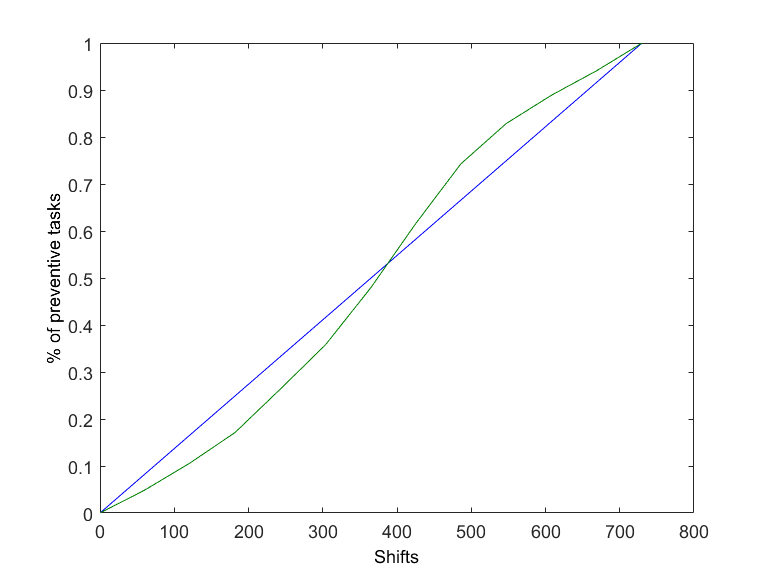
\includegraphics[scale=0.5]{EJOR/figures/developactivities.png}
	\end{center}
	\caption{Linear and monthly average approaches to guide scheduling preventive tasks}
	\label{fig:monthavg}
\end{figure}
$SPC_p$ refers to the proportion of the penalty costs based on the time pattern $p$ spends on its different tasks types. If, for instance, one of the tasks of $p$ constitutes $\beta$\% of the total time of a particular task type, the $\beta$\% of the penalty cost of that task type is counted. However, the penalty for not performing preventive tasks during the year is rather high and patterns consisting on those tasks could be overly chosen. One way to proceed could be to limit the number of  preventive tasks that can be scheduled linearly with time.  In that case, the number of preventive tasks of type $i$ that can be finished up by shift $t$ would be $ \frac{PP_it}{2T}$. However, gains can be obtained by scheduling more tasks when, seasonally, wind speed is expected to be slower. Performing preventive tasks when the wind speed is low saves downtime costs due to performing preventive tasks, as reflected by parameter $D_{st}$.
In practice, the weather conditions are not known to the planner beforehand, but the scheduler has insight in the monthly average conditions for wind speed, based on historic data. From these averages it can be derived the expected power loss for a single turbine during month $\tau$, which we assume to be captured by the average values $w_\tau$. One can normalise these values to obtain the proportion of expected loss of month $\tau$ respect to the total year: $\bar{w}_\tau=\frac{w_i}{\sum_{j=1}^{12}w_i}$. One would like to perform in month $\tau$ a fraction of the total planned preventive tasks that is inversely proportional to the number $\bar{w}_\tau$. This fraction is given by $\varphi_{\tau}=\frac{1}{\bar{w}_\tau}\frac{1}{\sum_{j=1}^{12}\bar{w}_j}$, dividing again by the total summation of $\bar{w}_j$ to normalise results.
%
Figure \ref{fig:monthavg} depicts the accumulative values of $\varphi_{t}$ interpolated between the month averages confronted with a linear approach.
%
Consequently, parameter BehindSch is determined for each $i\in \mathcal{NP}$ according to
$$BehindSch_{i}=\max((1-\varphi_{t})PP_i -\lceil \frac{RemainHours_i}{N_i}\rceil,0)$$
%
For corrective task types $i\in \mathcal{NC}$, we focus on the unfinished work
%
$$BehindSch_{i}= DownAct_i$$
%
Finally, to have a valuation $S{PC}_p$ for the pattern, we can add penalties $p_i$ leading to
%
$$SPC_p= \frac{t}{2T}\sum_{i \in \Gamma}p_iA_{ip}\frac{B_i}{N_i}Behindsch_i ,$$
%
Notice, this factor has a higher weight in the fitness when approaching the end of the horizon. However, if $Behindsch_i=0$ the valuation of $S{PC}_p$ is set to zero. If $Behindsch_i=0$ and for patterns that include one or more preventive type tasks, the wind speed is checked. In case it is lower than the expected average, the fitness valuation of $p$ is different: the pattern costs are not considered for the fitness and the number of hours of type $i$ that that pattern performs is calculated and subtracted from the fitness value.


The term \emph{scosts} is a negative value that refers to the potential savings in electricity production if a break down turbine is repaired. After calculating the contribution of pattern $p\in\mathcal{P}_{kv}$ for each  corrective task type $i\in \mathcal{NC}$ in terms of number of tasks performed, \emph{scosts} accumulates the value:
%
$$scosts=-nact(i)(2T-t)ydown$$
%
The term $ydown$ represents the average downtime cost of a single turbine for the total duration of the planning horizon. Notice, this factor gets a higher weight at the beginning of the planning horizon that than at the end.

% On Matlab, run script Untitled (I know...) to generate the data and the again.



%\subsection{Case $Behindsch_i=0$}
%\label{subsec:fitnessexception}
%For shifts in which preventive types are performed according to schedule, SPC does not count with the potentially saved costs for those types. $Behindsch_i=0$, the wind speed  is checked. In case is lower than the expected average, which is known, the pattern costs are not considered for the fitness. The number of hours of type $i$ that that pattern performs is calculated and subtracted from the fitness value.





%{algorithm}[h]
%	\caption{vesselcansail(Vessel $v$,shift $t$)}
%	\label{alg:vesselcansail}
%	\begin{algorithmic}
		%\REQUIRE say here
		%\ENSURE say here
%		\medskip
		%\FOR { $i\in \{1,\ldots,12/6\}$ (Change 12 and 6 for parameters)}
		%\STATE $n=12/6 (t-1)+i$
%		\RETURN {wind($n$)$<$maxWind($v$) AND wave($n$)$<$ maxWave($v$)}
		%\RETURN false;
		%\STATE EXIT;
		%\ENDIF
		
		%\ENDFOR
		%\RETURN true;
		%\STATE\RETURN return something?
		%\EndProcedure
		%\vskip 5pt
%	\end{algorithmic}
%\end{algorithm}


\section{Computational illustration}
\label{sec:computationalstudyEJOR}

In the MILP model, the lower level operational planning cost provides a lower bound for the incurred cost due to failures and downtime. By formulating the operational tasks in a one-shot model, in principle all the scenario is known beforehand and earlier tasks can be planned based on knowledge of failures that will occur later, i.e. anticipation is allowed. This makes the planning in principle cheaper than what is possible in reality. On the other hand, due to the  nature of the variable $\bar{w}_{its}$, there is a tension in the optimal outcome to start repairing a failure as soon as possible by a corrective task.

In this section, we discuss the amount of underestimation for specific realistic data confronting the optimal MILP outcome of the lower level for scenarios with the heuristic decision rule defined in Section \ref{sec:heuristic}.
%
The model and the heuristic have been compared for an instance similar to the one published in \cite{GutierrezAlcoba:ICCS2017}.

The MILP has been modelled for the bi-level model using GAMS interface \cite{gams}, and solved using the CPLEX solver, setting the optimality gap at 1\%.

\subsection{A case study}

We consider an OWF consisting of 125 turbines. The planning horizon is one year and the periods represent 12 hour shifts and include a return trip from the base the vessel is located to the OWF and a bundle of activities. In practical terms there are 730 periods. There are three available bases $B_1,B_2,B_3$ around the OWF, each of which can accommodate up to 48 technicians and they are located at 110, 61  and 86 kilometers respectively from the OWF. The cost of using each of them, for the entire time horizon is 2, 6 and 7 million monetary units (mu) respectively.

Four types of vessels are considered: $V_1,V_2,V_3,V_4$. Each base has space to allow two vessels of type $V_1$, two of type $V_2$, four of type $V_3$ and one of type $V_4$. Vessel type $V_4$ is able to accommodate up to 30 technicians, while the rest has space for only 12. The cost of having a vessel during the whole planning horizon for vessel types $V_1$, $V_2$, $V_3$ and $V_4$ is, respectively, 122,4000, 2,500,000, 750,000 and 7,200,000 mu. Vessel types $V_1$ and $V_2$ can travel at a speed of 20 knots, while vessel types $V_3$ and $V_4$ can travel at 40 knots. In practical terms this means that vessel types $V_1$ and $V_2$ require about 5.94, 3.3 and 4.64 hours to perform a return trip between bases $B_1$, $B_2$ and $B_3$ respectively while vessel types $V_3$ and $V_4$ would require half of that time, allowing more time to perform activities in each shift.

There are two preventive activity types $A_1,A_2$ and two corrective activity types $A_3, A_4$. All vessel types are able to perform all the activity types considered. Activity type $A_4$ requires the vessel supporting the operation to be present at the turbine while the activity is performed, whereas activity types $A_1,A_2,A_3$ can be run in parallel. The vessel drops a group of technicians at each turbine that is going to be supported during the shift. The time required to perform activity types $A_1$, $A_2$, $A_3$ and $A_4$ is 60 , 100 , 3 and 7.5 hours respectively. The maximum time per period and turbine that a group of technicians can support an activity type is 6 hours. Consequently, only activities of type $A_3$ can be performed in a single period. The penalty cost for not executing a preventive activity type is 10 million mu. For corrective activities of type $A_3$, the cost is 50,000 mu, and for type $A_4$, the penalty cost rises to 500,000 mu. The patterns for each combination of base and vessel type are generated following the procedure described in Algorithms \ref{alg:buildbundle} and \ref{alg:buildpattern}.

For our case study, there are 125 planned activities of type $A_1$ and 60 of type $A_2$. The number of corrective activity types corresponds to the number of failures of the turbines and depends on the scenario. A scenario consists of the events of the failures of the turbines and the weather conditions for every period. Failures that require corrective activity types $A_3$ and $A_4$ follow a binomial distribution. The rate of failures for a corrective activity of type $A_3$ is 5 times per turbine per year, and 3 times per turbine a year for failures that require an activity of type $A_4$. Weather conditions are taken from historical weather data. For each scenario, a report file containing a year of wind speed and wave height data of the OWF area is picked for feeding these variables.

\subsection{Discussion of results}

For comparing the performance of the heuristic for the operational stage with the optimal solution of the MILP problem, two different tactical stage decisions have been considered. The first one is  the optimal solution for the MILP, (S1), which consists of using three vessels of type $V_3$ from base $B_1$. An instance consisting on a tactical stage decision using less vessels than the optimal MILP solution based on perfect information, would not generate significant results. The second instance (S2) consists of using four vessels of type $V_3$ from base $B_1$.

A set of 20 scenarios have been generated. For each scenario, the heuristic has been run and the MILP problem has been solved for the tactical stage decisions studied, (S1) and (S2) the optimal solution for the MILP; using three vessels of type $V_3$ from base $B_1$ and (S2). Table \ref{tab:experiments} presents the average value of the 20 scenarios for the total cost, executing patterns cost, preventive and corrective downtime costs and operational stage costs for tactical stage decisions S1 and S2, running the heuristic and solving the MILP problem. Preventive and corrective penalty costs are not included in Table \ref{tab:experiments}, since they result to be zero for the generated scenarios.

\begin{table}[h]
	\centering
	\caption{Associated costs for the MILP optimal solution and the heuristic for tactical decisions S1 and S2}
	\label{tab:experiments}
\begin{tabular}{rrrrrr}
         & Total    & Pattern & P. D.   & C. D.   & Op. S. Cost \\
MILP S1  & 10986350 & 5060220 & 1117923 & 558265  & 6736408     \\
MILP S2  & 11472400 & 5126880 & 1028245 & 314890  & 6470015     \\
HEUR. S1 & 13401952 & 5346330 & 2296092 & 1509528 & 9151951     \\
HEUR. S2 & 12958671 & 5435595 & 1235124 & 1287951 & 7958671
\end{tabular}
\end{table}

The MILP complete information solution for S1 has a total cost of nearly 11 million monetary units (MU), while the heuristic for S1 has a cost of 13.4 million MU. Considering only the costs of the operational stage, the MILP complete information solution is 6.73 million MU, while the heuristic reaches 9.15 million MU. %For a few scenarios, the heuristic cannot finish all the preventive tasks, giving an average value for preventive penalty costs of 160000 MU.
Downtime costs for corrective tasks is about 2.7 times higher than the MILP cost. For preventive tasks the cost doubles that of the MILP solutions. This shows that the heuristic does not perform well for S1 with the optimal MILP perfect information setting. In a real setting, when failures and weather conditions are uncertain, that tactical decision might not be optimal.

However, for S2 the deviation between the two solutions is quite different. The MILP complete information solution for the operational stage is 6.47 million MU, reducing only slightly the costs of S1. However, the heuristic reduces that cost to 7.95 million MU, and this reduction comes mostly by handling preventive tasks much better, reducing the cost by half compared to the tactical decision S1. It can be observed that the downtime cost for corrective tasks, incurred by broken down turbines until they are repaired, is the only cost significantly higher for the heuristic compared to the MILP solution costs, for both tactical decisions S1 and S2. This can be explained considering that the MILP model has exact information for when the failures occur for all the periods of the problem, being able to anticipate corrective tasks early in time. In contrast, the cost of performing the patterns, which constitutes the major cost of operating the OWF and is not related with uncertain events, is only  6\% above the one provided by the MILP.





\section{Conclusion}
\label{sec:conclusion}
Models in the literature on selecting an optimal vessel fleet composition for operations and maintenance tasks at OWFs during a planning horizon typically apply a complete information approach to evaluate the fleet composition. The models are confronted with weather conditions and turbine failures. Weather conditions may prevent vessels sailing and execute tasks at the OWF, while turbine failures result in new corrective maintenance tasks. However, weather conditions and failures are unknown in practice. Therefore, a deterministic complete information approach to find the optimal solution for the operational stage only provides a lower bound on the maintenance costs in the operational stage. In the current paper, a similar MILP model for the fleet composition is presented. The question is: What are the costs if the scheduler applies a heuristic rule based on the information available in practice? This means, the heuristic is not based on perfect information, realising the weather and failure events at the beginning of each shift. The results show that the heuristic performs well  when the tactical decisions include enough vessels to cover the demand of O\&M activities at the OWF and allows for slack in the scheduling compared to the optimal complete information plan. Although the performance costs of the heuristic for the chosen scheduling are only 6\% above the optimal lower bound, for the corrective tasks, where (stochastic) failures have to be repaired, the cost is about four times higher than that given by the MILP. This illustrates the effect of anticipation in a perfect information situation. The value of evaluating the fleet composition in a realistic setting is that probably the chosen vessel plan will contain more vessels, as this facilitates recourse actions on random events.

%\bibliographystyle{plain}
%\bibliography{Tesis_Alejandro}


%\end{document}

\clearemptydoublepage

% this file is called up by thesis.tex
% content in this file will be fed into the main document

\chapter{Conclusions} % top level followed by section, subsection
\label{Chap:Contributions}

% ----------------------- paths to graphics ------------------------

% change according to folder and file names
\ifpdf
    \graphicspath{{8/figures/PNG/}{8/figures/PDF/}{8/figures/}}
\else
    \graphicspath{{8/figures/EPS/}{8/figures/}}
\fi

% ----------------------- contents from here ------------------------

This chapter summarises the findings of the works presented in this thesis and shows guidelines for possible future research.

We can distinguish two main areas of research in this thesis. The first one dealt with lot sizing problems for perishable items. The second, with the optimization of the maintenance processes at offshore wind farms. Each of them provided findings for the research questions investigated in this thesis, related to dynamic decision making.

The first research question of this thesis is to study which order policies are the most appropriate for a general lot sizing problem for a perishable item. Can the optimal policy be found? Chapter \ref{Chap:iccsa2015} describes that problem and discusses a solution method. The model studied is a lot sizing problem for a single perishable item following a static strategy over a finite time horizon and considering ordering, holding, unit and waste costs. Demand is stochastic and non-stationary, a $\beta$-service level for the demand is considered and a FIFO issuing policy is followed. For this problem setting theoretical properties were derived of the optimal solution aiding a possible solution approach. Moreover, a specific algorithm exploiting these properties has been developed to find an YQ policy derived for the static-dynamic case, using Monte Carlo simulation to estimate the expected value of the inventory levels. This policy proved to be optimal for the static-dynamic case. By enumerating the feasible timing order policies, the optimal solution for the static strategy can be found by finding the optimal quantities for each replenishment schedule. 

However, this solution method requires a high computational demand due to the Monte Carlo simulation and enumeration of replenishment schedules. This led to a new research question: How can the use of parallel computing improve the performance of the algorithms to find solutions for the problem? 

Two implementations were developed for heterogeneous platforms: a multi-GPU version using CUDA and a multicore version using Pthreads and MPI. For the multi-GPU version, the Monte Carlo simulation (the most demanding task of the solution method) was parallelised using the CUDA interface. For the multicore version, the initial approach for a multi-core parallelisation suggested an embarrassingly parallel implementation, as finding the optimal quantities for each replenishment schedule are in fact independent subproblems. However, randomly dividing the workload among processors led to an unbalanced workload for the processors. The reason behind this is that, rather than using Monte Carlo, an exact analytical approach to calculate the inventory levels for a cycle can be followed for the periods in which the inventory levels are equal to zero. Calculating the order quantities for a cycle analytically is much faster than using Monte Carlo simulation, even when using small samples. After identifying the computational workload of each replenishment schedule subproblem, balancing the workload among processors resembles a bin-packing problem. Three fast heuristics with reduced overhead were proposed for the bin-packing problem. The one that procured the best balancing in the testbed was used for parallelising the multicore version of the lot sizing problem.

The last research question concerning lot sizing problems involved considering the use of heuristics for such problems: to which extend does the use of heuristics give good results in a DDM lot sizing problem for perishable products? In this case, a similar lot sizing model was used. The difference with the former studied model is to use a penalty cost for unfulfilled demand, rather than using a $\beta$-service level and allowing backordering. For this model, exact analytical expressions to compute the expected value of the inventory for different product ages were found, assuming the product can age indefinitely. This derived an analytical approximation for the inventory levels for the case in which the product age is discrete and finite. From here, an extension of Silver's heuristic has been developed for the case of perishable products, introducing an analytical and a simulation-based variant of the approach. An SDP model for the problem was derived as well, in order to compare the optimal solution with the heuristic. Results showed that the simulation approach featured an average cost performance only 5\% above the optimal cost. For the analytical approximation this figure was 6\%.


%\item Is it possible to find an efficient and realistic metaheuristic for scheduling O\&M activities at offshore wind farms with failures and weather uncertainty? What are the differences with a perfect information MILP model?

A second practical dynamic decision making problem was studied for continuing the research in this thesis. The topic was related to optimising the maintenance activities at a OWF. Chapters \ref{Chap:iccs2017} and \ref{Chap:ejor} address this problem. The first research question is addressed in Chapter \ref{Chap:iccs2017}: is an MILP model suitable for an application for selecting a fleet of vessels to support the maintenance at offshore wind farms? A discrete, scenario based and deterministic optimisation model was derived, presented as a bi-level problem: On the first level, decisions are made in order to select a fleet of vessels. On the second level, the fleet is used to optimise the schedule of O\&M activities at a OWF, dealing with turbine failure events and considering weather conditions that may prevent performing activities for safety reasons. The model solves instances of more than 700 periods (The planning horizon is set to one year, deciding activities in twelve hours shifts). However, such a model is based on perfect information for failure events and weather conditions, since adding non-anticipative constraints would leave the model unsolvable. Previous models in literature, aiming to solve long time horizon problems using small time periods (\cite{HALVORSENWEARE2013}, \cite{Stalhane2016357}) are deterministic as well. This situation set new research questions, as the vessel fleet composition may be affected when maintenance scheduling is done when the failures events and the weather conditions are uncertain. 

The next research question was: Is it possible to find an efficient and realistic metaheuristic for scheduling O\&M activities at offshore wind farms with failures and weather uncertainty? What are the differences with a perfect information MILP model? Chapter \ref{Chap:ejor} discusses a heuristic that schedules the O\&M activities and shows to what extend a non-anticipative method affects the optimal solution. The experiments show that the optimal fleet composition given by the MILP model is not sufficient to operate the OWF efficiently using the heuristic. However, adding only an extra vessel provides a fair solution: the cost of performing the activities, which constitutes the major cost of operating the OWF and is not related with uncertain events, is only  6\% above the one provided by the MILP. In contrast, the cost associated with the downtime in turbines due to failure events, which are uncertain for the heuristic, are about three times higher than the given by the perfect information MILP model.



%anticipative, as 

%\subsection{Future research}
%\label{subsec:futureresearch}

% ---------------------------------------------------------------------------
%: ----------------------- end of thesis sub-document ------------------------
% ---------------------------------------------------------------------------










        % description of lab methods
\clearemptydoublepage	
%%%%%%%%%%%%gloria
%\pagestyle{fancy}
%\renewcommand{\chaptermark}[1]{\markboth{\MakeUppercase{\thechapter. #1 }}{}}
%\renewcommand{\sectionmark}[1]{\markright{\thesection\ #1}}
%\fancyhf{}
%\fancyhead[RO]{}
%\fancyhead[LE]{APPENDIX I}
%\fancyfoot[C]{\thepage}
%\renewcommand{\headrulewidth}{0.5pt}
%\renewcommand{\footrulewidth}{0pt}
%\addtolength{\headheight}{0.5pt}
%\fancypagestyle{plain}{
%  \fancyhead{}
%  \renewcommand{\headrulewidth}{0pt}
%}
\fancyhead[LE]{APPENDIX I}
\fancyfoot[C]{\thepage}
%%%%%%%%%%%%%%%%%%%

% this file is called up by thesis.tex
% content in this file will be fed into the main document

%: ----------------------- introduction file header -----------------------


\chapter*{Appendix I: Publications arising from this thesis}
\label{AppendixA}

The research work carried out for the present thesis resulted in a number of
publications. This appendix lists them along with their respective quality indicators
and sorted by their year of publication (oldest first) within each category.


\section*{Publications in International Journals (JCR)}

\begin{itemize}

\item [\cite{Gutierrez-Alcoba16}] \bibentry{Gutierrez-Alcoba16} 

Impact factor JCR 2016: 2.325. Q1 (Operations Research \& Management Science)

\item [\cite{GutierrezAlcoba201712}] \bibentry{GutierrezAlcoba201712} 

Impact factor JCR 2016: 1.93. Q2 (Computer Science, Theory \& Methods) 

\end{itemize}

\section*{Publications submitted to International Journals (JCR)}
\begin{itemize}
	\item [\cite{GutierrezAlcoba:EJOR2017}] \bibentry{GutierrezAlcoba:EJOR2017} 
	
%Impact factor JCR 2016: 3.297. Q1 (Operations Research \& Management Science)
	 	
\end{itemize}



\section*{Publications in International Journal (not JCR)}
\begin{itemize}
\item [\cite{GutierrezAlcoba:ICCS2017}]  \bibentry{GutierrezAlcoba:ICCS2017}
\end{itemize}

\section*{Publications in Book Chapters}
\begin{itemize}
\item [\cite{GutierrezAlcoba:ICCSA2015}] \bibentry{GutierrezAlcoba:ICCSA2015}
\end{itemize}

\section*{Publications in International Conferences}
\begin{itemize}
\item [\cite{GutierrezAlcoba:MAGO14}]  \bibentry{GutierrezAlcoba:MAGO14}
\item [\cite{GutierrezAlcoba:EURO15}]  \bibentry{GutierrezAlcoba:EURO15}
\item [\cite{GutierrezAlcoba:EUROPT15}]  \bibentry{GutierrezAlcoba:EUROPT15}
\item [\cite{GutierrezAlcoba:Segovia2017}]\bibentry{GutierrezAlcoba:Segovia2017}
\item [\cite{GutierrezAlcoba:OR2017}]\bibentry{GutierrezAlcoba:OR2017}
\end{itemize}

\section*{Publications in National Conferences}
\begin{itemize}
\item [\cite{GutierrezAlcoba:JP15}] \bibentry{GutierrezAlcoba:JP15}
\end{itemize}

% ----------------------------------------------------------------------




\addcontentsline{toc}{chapter}{Appendix I: Publications arising from this thesis}
\clearemptydoublepage

%%%%%%%%%%%%%%%%%%%%glo%ria
%\pagestyle{fancy}
%\renewcommand{\chaptermark}[1]{\markboth{\MakeUppercase{\thechapter. #1 }}{}}
%\renewcommand{\sectionmark}[1]{\markright{\thesection\ #1}}
%\fancyhf{}
%\fancyhead[RO]{}
%\fancyhead[LE]{APPENDIX II}
%\fancyfoot[C]{\thepage}
%\renewcommand{\headrulewidth}{0.5pt}
%\renewcommand{\footrulewidth}{0pt}
%\addtolength{\headheight}{0.5pt}
%\fancypagestyle{plain}{
%  \fancyhead{}
%  \renewcommand{\headrulewidth}{0pt}
%}
\fancyhead[LE]{APPENDIX II}
\fancyfoot[C]{\thepage}
%%%%%%%%%%%%%%%%%%%%%%%%%%%

% this file is called up by thesis.tex
% content in this file will be fed into the main document

%: ----------------------- introduction file header -----------------------
\chapter*{Appendix II: Other publications produced during the elaboration of this thesis}
\label{AppendixB}

The research effort invested during the time span in which this thesis was elaborated
produced additional publications as the result of other research lines
not included in the present dissertation. Those lines were Perishable Inventory Control and Procedural Content Generation using population based algorithms. This appendix
lists them along with theirs respective quality indicator.


\section*{Publications in International Journals}
\begin{itemize}
\item [\cite{PaulsWorm2015}] \bibentry{PaulsWorm2015}

Impact factor JCR 2016: 2.22. Q1 (Operations Research \& Management Science), Q1 (Economics and econometrics), Q1 (Industrial and Manufacturing 
Engineering)

\end{itemize}

\section*{Publications in Proceedings of International Conferences with DOI}
\begin{itemize}
\item [\cite{Lara-Cabrera2016}] \bibentry{Lara-Cabrera2016}
\item [\cite{Hendrix2015}] \bibentry{Hendrix2015}
\end{itemize}

\section*{Publications in other International Conferences}
\begin{itemize}
	\item [\cite{PaulsWormISIR2014}] \bibentry{PaulsWormISIR2014}
\end{itemize}
% ----------------------------------------------------------------------




\addcontentsline{toc}{chapter}{Appendix II: Other publications produced during the elaboration of this thesis}
\clearemptydoublepage

%%%%%%%%%%%%%%%%%%%%gloria
%\pagestyle{fancy}
%\renewcommand{\chaptermark}[1]{\markboth{\MakeUppercase{\thechapter. #1 }}{}}
%\renewcommand{\sectionmark}[1]{\markright{\thesection\ #1}}
%\fancyhf{}
%\fancyhead[RO]{}
%\fancyhead[LE]{RESUMEN EN ESPA\~NOL}
%\fancyfoot[C]{\thepage}
%\renewcommand{\headrulewidth}{0.5pt}
%\renewcommand{\footrulewidth}{0pt}
%\addtolength{\headheight}{0.5pt}
%\fancypagestyle{plain}{
%  \fancyhead{}
%  \renewcommand{\headrulewidth}{0pt}
%}
\fancyhead[LE]{RESUMEN EN ESPA\~NOL}
\fancyfoot[C]{\thepage}
%%%%%%%%%%%%%%%%%%%%%%%%%%%

%
%%%%%%%%%%%%%%%%%%%%%%%%%%%%%%%%%  ejemplo.tex %%%%%%%%%%%%%%%%%%%%%%%%%%%%%%%
%
%%%%%% Fichero de ejemplo LaTeX que ilustra el uso de la Hoja de Estilo %%%%%%
%%%%%% Jornadas.cls para Jornadas Sarteco.              %%%%%%
%
%\documentclass[twocolumn,twoside]{Jornadas}
%\usepackage[latin1]{inputenc}
%\usepackage[dvips]{epsfig}
%\usepackage{graphicx}
%\usepackage{amsmath}
%\usepackage{color}
%\usepackage{amssymb}
%\usepackage{graphicx}
%\usepackage{epstopdf}
%\usepackage{algorithm,algpseudocode}
%\usepackage{multirow}
%\usepackage{url}
%\usepackage{breakurl}
%\usepackage{hyperref}
%
%\def\FUNCT{{\bf Funct}\ }
%\def\PROC{{\bf Proc}\ }
%\def\AND{\mathrel{\,\text{\bf and }\,}}
%\def\OR{\mathrel{\,\text{\bf or }\,}}
%\def\NOT{\mathrel{\,\text{\bf not }\,}}
%\def\IF{{\bf if}\ }
%\def\ELSE{{\bf else}\ }
%\def\ELSIF{{\bf elsif}\ }
%\def\WHILE{{\bf while}\ }
%\def\DO{{\bf do}\ }
%\def\FOR{{\bf for}\ }
%\def\TO{{\bf to}\ }
%\def\RETURN{{\bf return}\ }
%\def\COMMENT{{\bf comment:}\ }
%
%
%
%\def\BibTeX{{\rm B\kern-.05em{\sc i\kern-.025em b}\kern-.08em
%    T\kern-.1667em\lower.7ex\hbox{E}\kern-.125emX}}
%
%\newtheorem{theorem}{Teorema}
%
%
%
%%%%%%%%%%%%%%%%%%%%%%%%%%%%%%%%%%%%%%%%%%%%%
%
%\hyphenation{pa-ra-le-lis-mo pro-cee-dings de-ma-sia-do Su-ge-ri-mos
%             mo-di-fi-ca-cio-nes afi-lia-cio-nes re-fe-ren-te co-men-ta-rios
%             usan-do pro-ble-ma plan-ti-lla}
%
%\begin{document}


%\title{Implementaciones paralelas para un problema de control de inventarios de productos perecederos}
%
%\author{%
%     Alejandro G. Alcoba, Eligius M.T. Hendrix, Inmaculada Garc\'ia%
%     \thanks{Computer Architecture, Universidad de M{\'a}laga, e-mail: {\tt \{agutierreza,eligius,igarciaf\}@uma.es}},
%      Gloria Ortega %
%     \thanks{Informatics, Univ. of Almer\'ia, Agrifood Campus of Int. Excell., ceiA3, e-mail: gloriaortega@ual.es {\tt }}
%      %Karin G.J. Pauls-Worm, Rene Haijema%
%     %\thanks{Operations Research and Logistics, Wageningen University, e-mail: {\tt }}
%}
%
%\maketitle
%% Oculta las cabeceras y los n\'umeros de p\'agina.
%% Ambos elemetos se a\~nadir\'an durante la edici\'on de las actas completas.
%\markboth{}{}
%\pagestyle{empty}
%\thispagestyle{empty} % Oculta el n\'umero de la primera p\'agina
%
%\begin{abstract}
%En este trabajo se analizan y eval\'uan dos implementaciones de un algoritmo de optimizaci\'on para un problema de control de inventarios de productos perecederos. Las implementaciones se han llevado a cabo utilizando una arquitectura heterog\'enea donde cada nodo est� compuesto por varios multicores y varias GPUs. Las versiones paralelas que se han desarrollado son: (1) una versi\'on MPI-PTHREADS  en la que se extrae el paralelismo tanto a nivel de proceso MPI como a nivel de hilo y (2) una versi\'on multiGPU en la que se obtiene el paralelismo a nivel de proceso MPI y a nivel de cores de GPU.
%Este algoritmo puede ser descompuesto f�cilmente en un conjunto de tareas que no presentan ninguna dependencia entre s\'i. Sin embargo, la carga computacional asociada a cada una de las tareas es diferente y el problema del reparto de las tareas entre los elementos de proceso se puede modelar como un problema de Bin Packing. Ello implica que la selecci\'on del conjunto de tareas asociadas a cada una de las unidades de computaci\'on requiere del dise\~no de heur\'isticas que sean capaces de balancear la carga eficientemente y de forma est\'atica. En este trabajo hemos analizado y evaluado varias heur\'isticas. Finalmente, la mejor heur\'istica ha sido la utilizada en la implementaci\'on paralela del algoritmo de control de inventarios que ha sido evaluado en la versi\'on MPI-PTHREADS y en la versi\'on multiGPU. Para la implementaci\'on MPI-PTHREADS los resultados obtenidos muestran una buena escalabilidad mientras que las versi\'on MultiGPU para el ejemplo que se ha evaluado deja de ser eficiente cuando se usan mas de 2 GPUs.
%\end{abstract}
%
%\begin{keywords}
%Multihilo, Multi-GPU, Bin Packing, Monte-Carlo, inventarios, productos perecederos.
%\end{keywords}
%\usepackage[utf8]{inputenc}
\chapter*{Resumen en espa\~nol}
\label{AppendixA}
%\ifpdf
%\graphicspath{{X/figures/PNG/}{X/figures/PDF/}{X/figures/}}
%\else
%\graphicspath{{X/figures/EPS/}{X/figures/}}
%\fi
\section*{Introducci\'on}
Esta tesis analiza aplicaciones de toma de decisiones din\'amica para un conjunto de problemas. Pueden diferenciarse dos l\'ineas principales. La primera trata problemas de gesti\'on de la cadena de suministro para productos perecederos, mientras que la segunda estudia el dise\~no de flotas de embarcaciones para realizar labores de mantenimiento en parques e\'olicos marinos. Los modelos de inventario para productos perecederos estudiados en esta tesis consideran un \'unico producto, una \'unica localizaci\'on de suministro y una planificaci\'on de producci\'on sobre un horizonte de tiempo finito.

Los principales objetivos de esta tesis son los siguientes: (1) estudiar que pol\'iticas de pedido son las m\'as apropiadas para los problemas de tama\~no de lote. ?`En qu\'e casos una pol\'itica de pedido da una soluci\'on \'optima?; (2) analizar el efecto del uso de computaci\'on paralela para mejorar el rendimiento de los algoritmos derivados y as\'i dise\~nar pol\'iticas para problemas de tama\~no de lote de productos perecederos; (3) explorar c\'omo de efectivas pueden ser las heur\'isticas para problemas de toma de decisiones din\'amica sobre el tama\~no de lote de productos perecederos; (4) elaborar un modelo MILP para seleccionar una flota de embarcaciones con el fin de realizar las operaciones de mantenimiento en parques e\'olicos marinos; y (5) dise\~nar una heur\'istica para programar las operaciones de mantenimiento en parques e\'olicos marinos considerando fallos en turbinas e incertidumbre meteorol\'ogica.


En el primer cap\'itulo de esta tesis se realiza una introducci\'on a la teor\'ia de control de inventarios y  se justifican las motivaciones que han llevado a cabo el desarrollo del trabajo que se incluye en esta tesis. Los cap\'itulos posteriores tratan independientemente cada uno del los objetivos anteriormente mencionados. En el segundo cap\'itulo, un modelo de programaci\'on estoc\'astica es presentado para un problema pr\'actico de planificaci\'on de producci\'on de un producto perecedero en un horizonte de tiempo finito. Una pol\'itica est\'atica es estudiada para el modelo. Tal pol\'itica ha demostrado ser \'optima asumiendo una estrategia de incertidumbre est\'atica, que es considerada para instancias con un tiempo de espera largo. El tercer cap\'itulo trata el uso de computaci\'on paralela para los algoritmos desarrollados en el cap\'itulo previo. Dos implementaciones fueron desarrolladas sobre plataformas heterog\'eneas: una versi\'on multi-GPU usando CUDA y una versi\'on multicore usando Pthreads y MPI. Para la primera implementaci\'on, la simulaci\'on de Monte Carlo (la tarea m\'as costosa), es paralelizada. Ambas implementaciones mostraron una buena escalabilidad. El cuarto cap\'itulo trata la efectividad de heur\'isticas para problemas de tama\~no de lote de productos perecederos similar. La cl\'asica heur\'istica de Silver es extendida para productos perecederos y se presentan variantes del procedimiento: una anal\'itica y una basada en simulaci\'on. Los resultados de la heur\'istica son comparados con las soluciones \'optimas dadas por un modelo SDP (Stochastic Dynamic Programming) generado para el problema, mostrando que los costes de las heur\'isticas presentan, de media, un 5\% sobre el coste \'optimo para la estrategia basada en simulaci\'on y un 6\% para la aproximaci\'on anal\'itica. En el quinto cap\'itulo, se presenta un modelo MILP para seleccionar la flota de embarcaciones \'optima para el mantenimiento de un parque e\'olico marino. El modelo se presenta como un problema de dos niveles, seleccionando la flota \'optima en el primer nivel y optimizando la selecci\'on de las operaciones, usando dicha flota, en el segundo. Dado que el modelo es determin\'istico, como otros en la literatura que aspiran a resolver problemas con un horizonte temporal largo usando periodos cortos, el sexto cap\'itulo trata la cuesti\'on de c\'omo la anticipaci\'on de los eventos estoc\'asticos como los fallos en las turbinas o las condiciones meteorol\'ogicas afectan la decisi\'on de la flota de embarcaciones \'optima. Este cap\'itulo presenta una heur\'istica que ilustra este efecto.








\section*{Resumen del cap\'itulo \ref{Chap:iccsa2015}}

La base de las implementaciones que se presentan en este cap\'itulo es un algoritmo desarrollado en Matlab para resolver un problema MINLP (Mixed Integer NonLinear Programming). Se trata de planificar, a lo largo de un n\'umero finito de periodos $T$, las cantidades que se deben proveer de cierto producto perecedero para satisfacer la demanda bajo una restricci\'on que establece un nivel de servicio $\beta$ que necesariamente se debe satisfacer. En concreto, esta restricci\'on establece que para cada periodo (siempre hablando en t\'erminos de esperanza matem\'atica) a lo sumo una fracci\'on $\beta$ de la demanda no pueda ser satisfecha y sea perdida por falta de stock, ya que se supone que esta no puede ser servida en un periodo posterior. Esta condici\'on es equivalente a que al menos una fracci\'on $(1-\beta)$ de la demanda sea cubierta en cada periodo. La duraci\'on de cada item producido desde que est\'a disponible para el consumidor hasta que ha de ser retirado es de $J<T$ periodos. Adem\'as, se supone que los productos se distribuyen siguiendo la regla FIFO: los productos son expedidos comenzando por los m\'as antiguos.

El problema de optimizaci\'on que se plantea es el de encontrar la cantidad de producto perecedero que hay que producir en cada periodo de forma que se satisfgan todas las restricciones del problema y que adem\'as se minimice una funci\'on coste.
A continuaci\'on se detallan las principales variables del modelo:

\smallskip\noindent\emph{\'Indices}\\
\begin{tabular}{ll}
	$t$ & \'indice del periodo, $t=1,\ldots,T$, siendo $T$ el  n\'umero total de periodos\\
	$j$ & \'indice de edad, $j=1,\ldots,J$, siendo $J$ la vida  \'util de cada unidad\\
\end{tabular}


\smallskip\noindent\emph{Par\'ametros}\\
\begin{tabular}{ll}
	$\boldsymbol{d}_t$ &
	\parbox[t]{13cm}{demanda en cada periodo con distribuci\'on
	normal dada por su media $\mu_t>0$ y varianza
	$(cv\times \mu_t)^2$ dado por un coeficiente de variaci\'on $cv$, id\'entico en cada periodo}\\
	$k$ & coste por periodo en el que se decide realizar  un pedido, $k>0$\\
	$c$ & coste unitario de producto, $c>0$\\
	$h$ & coste por almacenamiento, $h>0$\\
	$w$ & coste unitario de desecho, puede ser negativo  con la condici\'on, $w>-c$\\
	$\beta$ & nivel de servicio, $0<\beta<1$
\end{tabular}

%\noindent 5pt

\smallskip\noindent\emph{Variables}\\
\begin{tabular}{ll}
	$Q_t \ge 0$ & \parbox[t]{12cm}{cantidad de producto producido  y  disponible  en el periodo $t$.  Denotamos por $Q$ al vector completo $(Q_1,\ldots,Q_T)$}\\
	$Y_t \in \{0,1\}$ & \parbox[t]{12cm}{indica si se produce un pedido en el  periodo $t$. Es 1 si y solo si $Q_t>0$. Denotamos por $Y$ al vector completo  $(Y_1,\ldots,Y_T)$}\\
	$\boldsymbol{X}_t$ & ventas perdidas en el periodo $t$\\
	$\boldsymbol{I}_{jt}$ & \parbox[t]{12cm}{inventario de edad $j$ al final del  periodo $t$, considerando un  periodo  inicial fijo,  $I_{j0}=0$, $\boldsymbol{I}_{jt} \ge 0$  para $j=1,\ldots,J$}\\
\end{tabular}


\smallskip\noindent
Adem\'as, se usar\'a la notaci\'on $(\cdot)^+=max(\cdot,0)$.

\smallskip\noindent
La funci\'on coste que se pretende minimizar depende del vector  $Q=(Q_1,\ldots,Q_T)$ y se puede definir como:

\begin{equation}
\label{eq:obj}
f(Q)=\sum_{t=1}^T \left(C(Q_t) + E\left(h\sum_{j=1}^{J-1} \boldsymbol{I}_{jt}  +w\boldsymbol{I}_{Jt}\right)\right),
\end{equation}
siendo
\begin{equation}
\label{eq:proc}
C(x) = k+cx, \ \ \text{if} \ \ x>0,\ \text{and}\ \ C(0)=0
\end{equation}
El nivel de inventario para cada periodo $t=1,\ldots,T$  y cada edad $j$ siguiendo la regla FIFO puede calcularse como sigue: % en (\ref{eq:invWaste}) (\ref{eq:inv2}) y (\ref{eq:inv1}).

\begin{equation}
\label{eq:invWaste}
\boldsymbol{I}_{jt}=
\begin{cases}
\left(Q_t - (\boldsymbol{d}_t-\sum_{j=1}^{J-1}\boldsymbol{I}_{j,t-1})^+\right)^+ & j=1,\\
(\boldsymbol{I}_{J-1,t-1} - \boldsymbol{d}_t)^+ & j=J, \\
\left(\boldsymbol{I}_{j-1,t-1} - (\boldsymbol{d}_t-\sum_{i=j}^{J-1}\boldsymbol{I}_{i,t-1})^+\right)^+ & otro \ j%1<j<J
\end{cases}
\end{equation}


Por otra parte, la restricci\'on del nivel de servicio puede expresarse como:
\begin{equation}
\label{eq:chance}
E \left(\boldsymbol{X}_t\right) \le (1-\beta) \mu_t, \ t=1,\ldots,T
\end{equation}

Para controlar el cumplimiento de esta restricci\'on es necesario calcular las ventas perdidas que se producen en cada periodo $t$, lo cual viene dado por:
%
\begin{equation}
\label{eq:lostsales}
\boldsymbol{X}_t=\left(\boldsymbol{d}_t-\sum_{j=1}^{J-1}\boldsymbol{I}_{j,t-1}-Q_t\right)^+
\end{equation}
%
El valor esperado de las ventas perdidas es una funci\'on conocida como \emph{loss-function} que en general no admite una expresi\'on en t\'erminos elementales. Algunas aproximaciones factibles pueden verse en \cite{kurawarwala96,Rossi14,DeSchrijver20121375,Waissi199691}.
Para nuestro modelo hemos decidido utilizar la simulaci\'on Monte Carlo para obtener una estimaci\'on de la \emph{loss-function}.
Con las condiciones impuestas, el problema de encontrar las cantidades de producto perecedero que se deben producir en cada periodo y que minimizan la funci\'on coste $f(Q)$ dada en (\ref{eq:obj}), y con ello la pol\'itica $Y\in \{0,1\}^T$ de periodos de pedido \'optima, es un problema MINLP. Como veremos, la t\'ecnica usada presenta caracter\'isticas adecuadas para su implementaci\'on en computadores  de alto rendimiento.



\section*{Resumen del cap\'itulo \ref{Chap:jpdc}}
El objetivo de este cap\'itulo consiste en determinar hasta que punto el uso de una arquitectura heterog\'enea (multicore-multiGPU) facilita la resoluci\'on de un problema de optimizaci\'on del control de inventarios de productos perecederos. Pretendemos aprovechar la capacidad computacional de estas arquitecturas para obtener soluciones mas exactas, para ejemplos mas pesados desde el punto de vista de la computaci\'on, manteniendo tiempos de respuesta aceptables. El problema del control de inventarios queda definido a lo largo de una serie finita de $T$ periodos de tiempo en los que se ha de satisfacer la demanda (estoc\'astica) de un determinado producto perecedero que desde que se produce tiene una vida \'util de $J$ periodos. En el modelado de este problema se supone que la distribuci\'on se realiza siguiendo la pol\'itica de distribuci\'on FIFO, entregando el producto demandado con mayor  antig\"uedad. Se supone, adem\'as, que la demanda que no se satisfaga en un periodo queda perdida, no pudi\'endose acumular al periodo siguiente. La soluci\'on a este problema consiste en encontrar que cantidades de pedido a lo largo de todos los periodos resulta \'optima, en el sentido de minimizar el coste asociado a la producci\'on, distribuci\'on, almacenamiento y desecho de los productos que sobrepasen su vida \'util.

Actualmente, las arquitecturas de computaci\'on de altas prestaciones m\'as extendidas son las plataformas heterog\'eneas basadas en sistemas de
memoria distribuida, donde cada nodo tiene una arquitectura multicore que podr\'ia albergar un n\'umero distinto de cores~\cite{Hennessy12}. Por lo tanto, las implementaciones paralelas tienen que ser adaptadas para poder ser ejecutadas en dichas arquitecturas heterog\'eneas. En este contexto, es necesario tener un conocimiento detallado tanto del algoritmo a paralelizar como de los recursos computacionales que se van a utilizar para la implementaci\'on~\cite{Lastovetsky12}. Adem\'as, a estas arquitecturas se les pueden incorporar aceleradores, como son FPGAS, GPUs, coprocesadores Intel Xeon Phi, etc.
En concreto, en el problema del control de inventario para productos perecederos se ha optado por la combinaci\'on de cl\'usteres de Multi-GPUs. De este modo, el uso de plataformas masivamente paralelas (GPUs) permite la aceleraci\'on de las tareas computacionalmente m\'as costosas, porque estas unidades tienen mucha potencia de c\'alculo para los esquemas de computaci\'on vectorial. De forma adicional, el uso de plataformas de memoria distribuida permite obtener unos resultados m\'as precisos debido a que el uso de computaci\'on paralela permite incrementar el n\'umero de simulaciones realizadas para resolver un caso particular sin que el tiempo de ejecuci\'on se incremente.

El modelo de computaci\'on paralela asociado a este problema se puede  describir en t\'erminos de un conjunto de tareas que no presentan dependencias entre s\'i. Sin embargo, la carga computacional de cada una de estas tareas es variable y por lo tanto pueden aparecer problemas de desbalanceo de la carga si se hace un reparto de la carga a ciegas. Este problema de asignaci\'on de tareas a elementos de procesamiento se conoce en la literatura de complejidad como problema de Bin packing~\cite{Garey:1979:CIG:578533}. Dado que es un problema NP-Completo, se han desarrollado varias heur\'isticas que permiten tener una soluci\'on en un tiempo razonable.


El orden de complejidad del problema, partiendo del algoritmo secuencial, est\'a relacionado con el n\'umero vectores $Y$ (que indica los periodos en los que se realiza un pedido) posibles, lo cual depende de los valores de $J$ y $T$. Independientemente del valor de $J$, el n\'umero de casos posibles a tratar aumenta de forma exponencial con el valor de $T$, es decir, $O(e^T)$. M\'as a\'un, la complejidad para hallar las cantidades \'optimas de cada vector $Y$ depende del n\'umero de veces que es necesario recurrir a simulaci\'on de Monte Carlo, limitada a $T$ en cada caso. Cada vez que se realiza la simulai\'on, el inventario y las ventas perdidas son calculadas para $N$ casos independientes. Por tanto, el orden de complejidad para el m\'etodo completo, es decir, hallar el vector de pedidos $Y$ \'optimo y las cantidades \'optimas de pedido, es aproximadamente del orden de $O(N \cdot T \cdot e^T)$.


En la secci\'on anterior se ha puesto de manifiesto la necesidad de realizar simulaciones para obtener aproximaciones de la funci\'on \emph{floss}.
Esta funci\'on es la que consume la mayor parte del tiempo computacional de la ejecuci\'on del problema de inventarios.
Es importante destacar  la necesidad de realizar un elevado n\'umero de simulaciones para que las aproximaciones que lleva a cabo la funci\'on \emph{floss} sean suficientemente exactas.
Por tanto, para realizar aproximaciones relativamente precisas del valor de las ventas perdidas ($X$), es necesario realizar un  n\'umero $N$ de simulaciones del problema suficientemente alto, lo que constituye la verdadera carga computacional del problema. Como caso de estudio, se ha considerado un ejemplo del problema de control de inventarios en el que $T=15$ y $J=3$, que es bastante realista. Dicho ejemplo genera un total de 5768 vectores $Y$ posibles.




Una vez analizada la estructura algor\'itmica del problema, pasamos a describir los detalles de las implementaciones que hemos llevado a cabo sobre
 una arquitectura heterog\'enea formada por un cl\'uster de Multi-GPUs (multicores y dispositivos GPUs). El hecho de explotar una plataforma heterog\'enea de un cl\'uster tiene dos ventajas fundamentales: poder abordar la resoluci\'on de problemas de mayor tama\~no y reducir el tiempo de ejecuci\'on de un caso concreto. Las implementaciones consideradas en este trabajo han sido:

\begin{itemize}
	\item{MPI-PTHREADS:} Esta implementaci\'on obtiene el paralelismo de los procesadores multicore y de los nodos disponibles en el cl\'uster. Para ello, se utiliza programaci\'on basada en hebras~\cite{pthreads} y MPI~\cite{MPI}.
	\item{Multi-GPU:} Esta implementaci\'on est\'a basada en el uso de GPUs para realizar las simulaciones de Monte Carlo, las cuales son  la parte computacionalmente m\'as costosa del problema a resolver. Para ello, la interfaz de programaci\'on que se utiliza es CUDA.
\end{itemize}


Centrando nuestra atenci\'on en la implementaci\'on MPI-PTHREADS, se ha explotado el paralelismo en dos niveles: a nivel de nodo (memoria distribuida) y a nivel de multicore (memoria compartida).
Por un lado, existen m\'ultiples formas de paralelizar rutinas en modelos de memoria compartida, aunque la librer\'ia est\'andar es Pthreads (POSIX threads). Pthreads provee un conjunto unificado de rutinas en una librer\'ia de C cuyo principal objetivo es facilitar la implementaci\'on de threads o hilos en el programa.
Por otro lado, debido a su portabilidad, MPI ha sido el interfaz considerado para explotar el paralelismo a nivel de nodo.

Partiendo del algoritmo de optimizaci\'on del problema de inventarios, se ha realizado una paralelizaci\'on h\'ibrida (MPI y Pthreads), en la cual el conjunto de vectores $Y$ que se van a evaluar en el problema de  optimizaci\'on son repartidos entre los procesadores de acuerdo a las heur\'isticas de balanceo de la carga propuestas. La evaluaci\'on de esta implementaci\'on se ha realizado en un cl\'uster Bullx y los resultados se describen en las figuras \ref{fig:MPIPthreadsorder} y \ref{fig:SpeedUpMPIPthread} del cap\'itulo \ref{Chap:jpdc}.


 El reparto inicial de la carga de trabajo entre los procesadores disponibles puede considerarse como un problema de Bin packing con algunas restricciones. El problema de Bin packing se enmarca dentro de la optimizaci\'on combinatoria (NP-completo), y en nuestro caso se puede modelar de la siguiente forma: Dado un conjunto de $E$ ejecuciones independientes
del Algoritmo~\ref{alg:optimalforY} (items), cada una de ellas con una carga computacional $0<w_i< B$ y dado un conjunto de $P$ procesadores (Bins), repartir las ejecuciones del algoritmo entre los procesadores de forma que la carga computacional m\'axima asignada a un procesador sea m\'inima (ver \cite{Garey:1979:CIG:578533} para una formulaci\'on general del problema de Bin packing).

Debido a la dificultad de encontrar soluciones \'optimas para este tipo de problemas, habitualmente se utilizan t\'ecnicas heur\'isticas y metaheur\'isticas, que son capaces de encontrar una soluci\'on aceptable en un tiempo razonable. Algunas de estas heur\'isticas est\'an inspiradas en computaci\'on evolutiva~\cite{Blum:2003:MCO:937503.937505}.
Para resolver el problema de balanceo de la carga que se ha modelado como un problema de tipo Bin packing, proponemos tres algoritmos heur\'isticos (H1, H2 y H3) para repartir la carga de trabajo (en nuestro caso, los posibles vectores $Y$) entre todos los elementos de procesamiento disponibles de forma que se minimice el tiempo de ejecuci\'on del problema de optimizaci\'on.

\begin{enumerate}
	\item (H1): Heur\'istica basada en Round Robin: Ordenando previamente, de mayor a menor, el peso de las tareas a asignar, estas se reparten entre los $P$ procesadores siguiendo el patr\'on $(1,\ldots,P,P,P-1,\ldots,1,1,\ldots)$
	\item (H2): Heur\'istica basada en asignar sucesivamente los items $w_i$ al procesador  que menos carga de trabajo haya acumulado.
	\item (H3): Similar a la heur\'istica H2, pero previamente ordenando los items de mayor a menor carga.
\end{enumerate}

Para valorar las heur\'isticas se han utilizado tres instancias del problema denominadas $\gamma_1$, $\gamma_2$ y U, en las que la carga computacional estimada que se asocia a cada vector $Y$ es diferente. ($\gamma_1$) y ($\gamma_2$) est\'an basadas en distribuciones gamma con par\'ametros de forma y escala (10,4) y (1,25), respectivamente, y (U) sigue una distribuci\'on uniforme con valores entre 0 y 100.




Para medir el grado de balanceo de la carga asignada a cada procesador, se ha utilizado el coeficiente de Gini ($G$), ampliamente utilizado en el campo de la econom\'ia para medir el grado de desigualdad de la distribuci\'on de la riqueza en poblaciones~\cite{Gini0}. Este \'indice var\'ia entre 0 (equidad absoluta) y 1 (un solo individuo (procesador) posea toda la riqueza de la poblaci\'on (carga computacional)). $G$ se define como la media de la diferencia entre cada posible par de procesadores, divididos por su carga media. Para un n\'umero de ejecuciones $E$ asignadas a $P$ elementos de proceso, siendo $w_i$ la carga computacional asignada al procesador $i$, ordenadas de forma ascendente, $G$ se calcula como sigue:
%
\begin{equation}
	G= \frac{2\sum\limits_{i=1}^{P} i \cdot w_i}{P\sum\limits_{i=1}^{P}w_i}-\frac{P+1}{P}
\end{equation}
%
Gr\'aficamente, $G$ representa el ratio entre la diferencia del \'area rodeada por la l\'inea de uniformidad y la curva de Lorenz de la distribuci\'on, y el
\'area triangular que hay debajo de la l\'inea de uniformidad.
$G$ toma valores entre un m\'inimo de 0, cuando todos los procesadores tienen la misma carga, a un m\'aximo de 1, cuando todos los procesadores (excepto uno) tienen una carga de cero. Por lo tanto, cuando $G$ se acerca a 0 la carga est\'a bien balanceada, y cuando se acerca a 1 est\'a desbalanceada.




En la Tabla~\ref{tab:heurperformance} se resume el comportamiento de las diferentes heur\'isticas a trav\'es del valor del coeficiente de Gini ($G$) para los ejemplos planteados (compar\'andolos con un reparto a ciegas. Claramente se demuestra en esta tabla que la heur\'istica H3 es, al menos, un orden de magnitud mejor que las heur\'isticas H1 y H2 y que el reparto aleatorio de las tareas entre los procesadores (HR) es al menos dos ordenes de magnitud peor que H3 y un orden de magnitud peor que H1 y H2. De los datos de la Tabla \ref{tab:heurperformance}, se concluye que la heur\'istica H3 es la que presenta mejores resultados, consiguiendo balancear la carga de forma casi exacta, por lo tanto esta es la heur\'istica que produce mejores tiempos de ejecuci\'on en la evaluaci\'on de las implementaciones paralelas del problema del control de inventarios.




La versi\'on Multi-GPU se ha basado en la explotaci\'on de diversas GPUs para la paralelizaci\'on de las simulaciones del m\'etodo de Monte Carlo, realizadas por la funci\'on \emph{flossGPU} (ver Algoritmo~\ref{alg:cuda}). Por una parte, cada una de las $N$ simulaciones son independientes entre s\'i. Al mismo tiempo, para el c\'alculo de todo el inventario de cada una de las posibles edades~(\ref{eq:invWaste}), este solo depende del inventario del periodo anterior. Por tanto, separando por periodos, un kernel de CUDA puede realizar en paralelo el c\'alculo de las $N$ simulaciones y, al mismo tiempo, la actualizaci\'on del inventario de $J$ edades diferentes. Por tanto, la computaci\'on que se realiza con la GPU es la simulaci\'on de Monte Carlo. Al mismo tiempo, el modelo se ha implementado de forma que cada proceso MPI abre uno o dos hilos, que a su vez abren una o dos GPUs del nodo en el que se encuentra. Las tareas se reparten usando la heur\'istica (H3) entre las GPUs que se vayan a utilizar en cada caso.

El Algoritmo~\ref{alg:cuda} resume el cambio realizado en el Algoritmo \ref{alg:simulation} para adaptarlo a su ejecuci\'on en una o varias GPU. Tal y como se ha mencionado, el bucle que recorre los periodos se sit\'ua en el primer nivel.


Para la evaluaci\'on de las implementaciones paralelas hemos utilizado un cl\'uster compuesto de ocho nodos Bullx R424-E3 Intel Xeon E5 2650 (cada uno con 16
cores), interconectados por un puerto InfiniBand QDR/FDR embebido en la placa madre,
 8-GB RAM y 16-GB SSD) con ocho GPUs TeslaM2075 (de los ocho nodos, cuatro de ellos tienen dos GPUs por nodo). El driver de CUDA que se ha utilizado es CUDA 6.5. La arquitectura Multi-GPU y las caracter\'isticas de las GPUs se muestran en la Figura \ref{Tab:charGPU}.


En cuanto a la paralelizaci\'on MPI-PTHREADS, en la Figura \ref{fig:SpeedUpMPIPthread} se puede apreciar un buen nivel de speed-up. La rapidez con la que las heur\'isticas se ejecutan las hace apropiadas incluso para problemas en los que el desbalanceo no es muy acusado, mejorando un reparto aleatorio de las tareas. Para casos en los que el desbalanceo es mucho mayor (ejemplos con las distribuciones gamma y uniforme) el beneficio es mucho mayor y se observa que la heur\'istica (H3) presenta mejores resultados.

Con respecto a la implementaci\'on Multi-GPU, en la Tabla~\ref{tab:GPU} se recogen los tiempos de ejecuci\'on del problema completo, tomando hasta las 8 GPUs existentes en el cl\'uster para la paralelizaci\'on del m\'etodo Monte Carlo en CUDA. En dicha tabla se aprecia como se pueden conseguir buenos resultados paralelizando una escasa porci\'on del c\'odigo. En cambio, al usar m\'ultiples GPUs, la escalabilidad est\'a penalizada por el tiempo de inicializaci\'on de las GPUs (aproximadamente 5 segundos), lo cual hace que no se obtenga un buen rendimiento con m\'as de 2 GPUs para este ejemplo concreto. Para el ejemplo de inventarios considerado, el uso de los diecis\'eis cores de un solo nodo resulta m\'as beneficioso que el uso de las dos GPUs disponibles. En definitiva, la escalabilidad con el uso de m\'ultiples GPUs se ve limitada por el tiempo de inicializaci\'on requerido, aunque podr\'ia ser beneficiosa en comparaci\'on con la paralelizaci\'on MPI-PTHREADS si el problema a tratar requiere  m\'as precisi\'on, siendo necesarias m\'as simulaciones del m\'etodo de Monte Carlo, de forma que el tiempo de inicializaci\'on de las GPUs se hiciera comparativamente irrelevante.


\section*{Resumen  del cap\'itulo \ref{Chap:ijpr}}

Mientras que en el cap\'itulo \ref{Chap:iccsa2015} se describ\'ia un problema de control de inventarios para productos perecederos y un m\'etodo para encontrar su soluci\'on \'optima, el cap\'itulo \ref{Chap:jpdc} explotaba el uso de computaci\'on paralela en plataformas heterog\'eneas basadas en sistemas de memoria distribuida para acelerar la resoluci\'on del problema. No obstante, dicho m\'etodo se ve limitado por el hecho de incrementar, de forma exponencial, el c\'omputo necesario para hallar la soluci\'on \'optima seg\'un aumenta el n\'umero de periodos del problema.

En este cap\'itulo se proponen heur\'isticas que encuentran soluciones cuyo coste, de media, es solo un 5\% superior a al \'optimo. M\'as en concreto, este cap\'itulo realiza las siguientes contribuciones a la literatura de control de inventarios no perecederos con demanda estoc\'astica y no estacionaria:

\begin{itemize}
	\item Se introducen expresiones anal\'iticas exactas para realizar el c\'alculo  del valor esperado de inventario de diferentes edades cuando el producto puede envejecer indefinidamente; estas expresiones sirven tanto para distribuciones discretas como continuas para la demanda.
	\item Se derivan aproximaciones anal\'iticas para el caso en el que la edad l\'imite de los productos es discreta y finita.
	\item Utilizando estos resultados, se propone una extensi\'on de la heur\'istica de Silver\citep{citeulike:7292564} para el caso concreto de productos perecederos; en particular introduciomos una variaci\'on anal\'itica y otra basada en simulaci\'on para el procedimiento.
	\item Se realiza un estudio computacional con un extenso conjunto de datos que prueban que las heur\'isticas propuestas encuentran soluciones cuyo coste, de media, es solo un 5\% superior al \'optimo.
\end{itemize}

En este caso consideramos un problema de producci\'on de un \'unico producto, una \'unica localizaci\'on de suministro y una planificaci\'on de producci\'on sobre un horizonte de $T$ periodos. El producto considerado es perecedero y su edad, en periodos, se denota por  $a\in \{1,\ldots,A\};$ $a=1$ denota los productos nuevos reci\'en llegados al principio del periodo actual. Al final de un periodo dado $t$, todos los productos de edad $A$ son descartados; consideraremos $A<T$ para asegurar que el car\'acter perecedero de los productos afecta al modelo.

La demanda es estoc\'astica y no estacionaria, es decir, su distribuci\'on var\'ia entre periodos. La demanda en el periodo $t$ es una variable aleatoria no negativa $D_t$ con funci\'on de distribuci\'on conocida $F_t$. La distribuci\'on de estas variables aleatorias se supone independiente entre los periodos. Los productos se distribuyen siguiendo la regla FIFO. La demanda que no pueda satisfacerse no se considera perdida en este caso, sino que es satisfecha en el periodo siguiente. Suponemos que el tiempo de entrega de los productos es cero, aunque las heur\'isticas propuestas pueden adaptarse facilmente al caso en el que el tiempo de suministro es mayor.

Existe un coste fijo por ordenar un pedido $o$ y un coste $v$ proporcional a la cantidad de pedido solicitada; un coste por almacenamiento $h$ por cada producto que es llevado de un periodo al siguiente, independientemente de su edad; se incurre un coste de penalizaci\'on $p$ por cada unidad de demanda no satisfecha en cada periodo; un coste de desecho $w$ por cada producto de edad $A$ que sea descartado al final de cada periodo. El objetivo es encontrar una pol\'itica de suministro que minimice el coste total esperado, que est\'a compuesto por los costes de pedido, los costes de almacenamiento y los costes de penalizaci\'on y desecho, a lo largo del horizonte de $T$ periodos planificado.

Consideremos el inventario neto como el inventario almacenado menos la posible cantidad de demanda no satisfecha. El modelo supone que los eventos en cada periodo se suceden como se describe a continuaci\'on. Al comienzo de un periodo el inventario de distintas edades es observado. Si es necesario se produce un pedido de producto por la cantidad deseada. Tras esto, la demanda es observada y los niveles de inventario son actualizados siguiendo la regla FIFO. Tras esto, los productos de edad $A$ que queden en stock son descartados y se incurre un coste de desecho por ellos. Si por el contrario el inventario neto fuese negativo se incurre un coste de penalizaci\'on por la demanda no satisfecha. La Tabla \ref{tab:notation} del cap\'itulo \ref{Chap:ijpr} recoge la notaci\'on de par\'ametros y otras variables usada durante este cap\'itulo.

Los lemas \ref{lem:lemma1IJPR}-\ref{lem:lemma5IJPR} del cap\'itulo \ref{Chap:ijpr} muestran como obtener expresiones anal\'iticas para la esperanza de los diferentes niveles de inventario para el caso en el que el producto pueda envejecer indefinidamente. Esto sirve de base para obtener aproximaciones anal\'iticas para el caso de productos perecederos.

Nuestra heur\'istica hace uso de estos resultados para calcular, dado un inventario inicial $\mathbf{I}_{t-1},$ los niveles de inventario $\mathrm{E}(\mathbf{I}_t)$ durante el ciclo $t\in\{t,\ldots,r\}.$ Usando el lema \ref{lem:convexity} calcula la cantidad de pedido \'optima  $Q_t$ para el ciclo $(t,r)$ as\'i como la esperanza de los costes totales por periodo.

Como en la heur\'istica de Silver, se incrementa el valor de $r,$ empezando por $t,$ hasta que la esperanza de los costes totales por periodo asociados al ciclo $(t,r)$ aumenta por primera vez. Sea $r+1$ tal valor. La acci\'on \'optima en el periodo  $t$ es pedir una cantidad $Q_t$ que minimiza la esperanza de los costes totales para el ciclo $(t,r).$ Un pseudoc\'odigo del algoritmo puede consultarse en el Algoritmo \ref{algorithm_1}.

La tabla \ref{tab:pivot} muestra un resumen de los resultados obtenidos en nuestro estudio computacional. En dicha tabla se observa como la heur\'istica que hace uso de simulaci\'on se comporta, por lo general, mejor que la aproximaci\'on anal\'itica. No obstante, esta \'ultima es 10 veces m\'as r\'apida que la primera. De media, la heur\'istica anal\'itica encuentra soluciones cuyo coste es, de media, 5.96\% por encima del coste \'optimo para las 54 instancias, mientras que la heur\'istica que hace uso de simulaci\'on reduce esta diferencia al 4.76\%.


\section*{Resumen de los cap\'itulos \ref{Chap:iccs2017} y \ref{Chap:ejor}}

El problema de toma de decisiones para programar las operaciones de mantenimiento en parques e\'olicos marinos es tratado como un problema de cadena de suministro: la instalaci\'on requiere programar operaciones de mantenimiento y atender los fallos en turbinas durante el horizonte planificado. Una flota de embarcaciones tiene que ser seleccionada para realizar estas operaciones. Para este conjunto de problemas, las decisiones no son solo din\'amicas, sino que adem\'as se realizan bajo incertidumbre.

El problema de la planificaci\'on del mantenimiento de un parque e\'olico marino mediante una flota de embarcaciones propuesto en los cap\'itulos \ref{Chap:iccs2017} y \ref{Chap:ejor} est\'a basado en un modelo descrito en \cite{Elin}. El prop\'osito es encontrar la flota \'optima de embarcaciones y una colecci\'on de actividades de mantenimiento en las turbinas e\'olicas. El modelo contiene una descripci\'on detallada de la planificaci\'on de las operaciones relativas a cada acci\'on individual.

Se consideran actividades de mantenimiento preventivas y correctivas. Las actividades preventivas son aquellas que est\'an destinadas a prolongar la vida \'util de las turbinas e\'olicas y a prevenir fallos. Las actividades correctivas son aquellas destinadas a resolver fallos en las turbinas. Existe una corresponcencia biun\'ivoca entre los posibles fallos en las turbinas y los tipos de actividades correctivas del modelo.

El n\'umero de actividades preventivas de cada tipo que debe ser realizado durante la planificaci\'on temporal est\'a predefinido de antemano y este tipo de actividades pueden realizarse en cualquier periodo siempre que las condiciones meteorol\'ogicas lo permitan. Sin embargo, las actividades correctivas solo pueden realizarse desde el periodo en el que un determinado fallo ocurrre en una turbina e\'olica. Los fallos en turbinas se presentan por escenarios. Existe un coste por inactividad relativo a la p\'erdida de producci\'on energ\'etica en las turbinas durante la ejecuci\'on de cualquier tipo de actividad de mantenimiento. Asimismo, se consideran costes por inactividad para las turbinas averiadas, que se incurre hasta que se produce la reparaci\'on.

Para realizar las actividades de mantenimiento es necesaria una flota de embarcaciones. Los diferentes tipos de embarcaciones tienen propiedades como la clase de actividades que pueden realizar, capacidad para transportar a los t\'ecnicos, un coste de depreciaci\'on anual, una determinada velocidad de crucero y un l\'imite para el nivel de velocidad del viento y oleaje para los que es seguro navegar. Cada embarcaci\'on est\'a asociada a una base, desde la que viaja al parque e\'olico para realizar las actividades. Cada base tiene una determinada capacidad de embarcaciones, t\'ecnicos, un coste asociado y el valor de la distancia hacia el parque e\'olico.

El problema de decisi\'on incluye un n\'umero de bases posibles y un n\'umero de tipos de embarcaciones asociadas a ellas. Cada tipo de embarcaci\'on es capaz de realizar un determinado conjunto de patrones de actividades de mantenimiento desde la base a la que est\'a asociada. Un patr\'on consiste en una o varias actividades de mantenimiento que ser\'an realizadas en el parque e\'olico durante un periodo, incluyendo el tiempo que conlleva realizar un viaje de ida y vuelta de la base al parque e\'olico. En cada periodo las embarcaciones disponibles pueden realizar un patr\'on de los disponibles asociados al tipo de embarcaci\'on y a la base. Algunos patrones de distintas embarcaciones y asociados a distintas bases pueden ser virtualmente los mismos, conteniendo la misma lista de actividades a ser realizadas durante el periodo. El coste y el tiempo puede variar, considerando la velocidad de crucerod e cada embarcaci\'on o la distancia entre la base y el parque. Algunos tipos de actividades no requieren que la embarcaci\'on est\'e presente durante la actividad. Esto permite que varias actividades puedan ser ejecutadas paralelamente en un mismo periodo. Es irrelevante si un patr\'on contiene actividades que pueden ejecutarse en paralelo o no, siempre y cuando cumplan con las restricciones de tiempo durante un periodo y la embarcaci\'on permita transportar al n\'umero necesario de t\'ecnicos para realizar todas las actividades. M\'as a\'un, algunos tipos de actividades pueden llevar m\'as del tiempo disponible en un periodo. Estos tipos son cortados en peque\~nas partes que puedan ser realizadas durante los periodos. Si una actividad larga es iniciada en un determinado periodo, no es necesario que sea continuada en los siguientes. Sin embargo, para actividades de tipo correctivo, los costes por inactividad son incurridos en todos los periodos hasta que la actividad es finalizada y la turbina queda reparada.

Las decisiones del modelo tienen lugar en dos niveles: en un primer nivel (t\'actico) se deciden las bases y las embarcaciones que van a ser usadas durante la planificaci\'on temporal. El segundo nivel (operacional) programa las operaciones, incluyendo los patrones que realizar\'a cada embarcaci\'on disponible durante cada uno de los periodos. Los eventos aleatorios incluyen las condiciones meteorol\'ogicas que pueden prevenir el uso de las embarcaciones y los posibles fallos en turbinas que tienen lugar durante la planificaci\'on.

La formulaci\'on matem\'atica del modelo del cap\'itulo \ref{Chap:iccs2017} se encuentra recogida en la secci\'on \ref{sec:mathematicalformulationICCS}. Esta formulaci\'on matem\'atica no incluye las restricciones meteorol\'ogicas que prev\'en el uso de embarcaciones. Es en el cap\'itulo \ref{Chap:ejor} en la secci\'on   \ref{sec:mathematicalformulation} donde la formulaci\'on matem\'atica del problema MILP (Mixed Integer Linear Programming) es refinada, incluyendo estas nuevas restricciones. Del mismo modo, el cap\'itulo \ref{Chap:ejor} incluye, en la secci\'on \ref{subsec:buildpatterns}, una descripci\'on de los algoritmos recursivos usados para generar autom\'aticamente todos los patrones posibles para cada combinaci\'on de base y tipo de embarcaci\'on considerando las restricciones del problema.

El cap\'itulo \ref{Chap:ejor} incluye una heur\'istica para la fase operacional del modelo. Esta heur\'istica no realiza anticipaci\'on sobre los eventos aleatorios como la formulaci\'on MILP y es por tanto m\'as realista. En resumen, la heur\'istica consiste en un planificador de tareas que observa, al comienzo de cada periodo, los eventos de los nuevos fallos en turbinas y las condiciones meteorol\'ogicas. En funci\'on de ellos, toma decisiones sobre las embarcaciones a usar durante cada periodo y los patrones a realizar. Para ello, eval\'ua cada una de las posibles decisiones seg\'un una funci\'on de fitness y selecciona las decisiones de menor coste, incluyendo el estado ocioso de las embarcaciones.

%\section*{Agradecimientos}
%Alejandro G. Alcoba es becario del programa FPI. Este trabajo ha sido financiado por el Ministerio de Ciencia (TIN2012-37483) y la Junta de Andaluc\'ia (P11-TIC7176), parcialmente financiados por el Fondo Europeo de Desarrollo Regional (FEDER).


%\bibliographystyle{Jornadas}
%\bibliography{bibInventory}



%\end{document}


\addcontentsline{toc}{chapter}{Resumen en espa\~nol}
\clearemptydoublepage

%%%%%%%%%%%%%%%%%%%%bibliography gloria
%\pagestyle{fancy}
%\renewcommand{\chaptermark}[1]{\markboth{\MakeUppercase{\thechapter. #1 }}{}}
%\renewcommand{\sectionmark}[1]{\markright{\thesection\ #1}}
%\fancyhf{}
%\fancyhead[RO]{}
%\fancyhead[LE]{BIBLIOGRAPHY}
%\fancyfoot[C]{\thepage}
%\renewcommand{\headrulewidth}{0.5pt}
%\renewcommand{\footrulewidth}{0pt}
%\addtolength{\headheight}{0.5pt}
%\fancypagestyle{plain}{
%  \fancyhead{}
%  \renewcommand{\headrulewidth}{0pt}
%}

\fancyhead[RO]{}
\fancyhead[LE]{BIBLIOGRAPHY}
\fancyfoot[C]{\thepage}

\renewcommand{\bibname}{Bibliography} % changes the header; default: Bibliography
\bibliographystyle{plainurl}%{wileyj}
\bibliography{9_backmatter/references} % adjust this to fit your BibTex file

% the back matter: appendix and references close the thesis


\end{document}
